\documentclass[12pt]{mitthesis}
\usepackage{formatting}
% colors
\definecolor{g_color}{HTML}{3399CC}
\definecolor{e_color}{HTML}{FF3333}
\definecolor{oa_color}{HTML}{7400FF}
\definecolor{ob_color}{HTML}{FF00BA}
\definecolor{oc_color}{HTML}{EDA100}
\definecolor{od_color}{HTML}{00C49E}
\definecolor{hole_color}{HTML}{009999}
\definecolor{electron_color}{HTML}{FF0099}
\newcommand{\cg}[1]{\textcolor{g_color}{#1}}
\newcommand{\ce}[1]{\textcolor{e_color}{#1}}
\newcommand{\coa}[1]{\textcolor{oa_color}{#1}}
\newcommand{\cob}[1]{\textcolor{ob_color}{#1}}
\newcommand{\coc}[1]{\textcolor{oc_color}{#1}}
\newcommand{\cod}[1]{\textcolor{od_color}{#1}}
\newcommand{\eC}[1]{\textcolor{electron_color}{#1}}
\newcommand{\hC}[1]{\textcolor{hole_color}{#1}}

% units

% other commands
\newcommand{\hl}[1]{\textcolor{black}{#1}}
\newcommand{\bl}[1]{\textcolor{blue}{#1}}

% ----- electron variables -----
% k
\newcommand{\vf}{v_\mathrm{F}}
\newcommand{\kf}{k_\mathrm{F}}
% \mu

% ----- microwaves -----
% \omega
% f

% ----- bias knobs -----
\newcommand{\Vg}{V_\mathrm{c}}
\newcommand{\Vnw}{V_\mathrm{p}}
%\Phi

% ----- BCS -----
% \Delta
% \xi
% \varphi
% 

% ----- Andreev levels: general -----
\newcommand{\rA}{r_\mathrm{A}}
\newcommand{\pA}{\phi_\mathrm{A}}
\newcommand{\JA}{J_\mathrm{A}}
\newcommand{\HA}{H_\mathrm{A}}

% ----- weak link properties -----
% L
\newcommand{\pp}{\phi_\mathrm{p}}
% r
% \tau, channel transparency
% \phi_r reflection phase
% t
\newcommand{\Se}{S_\mathrm{e}}
\newcommand{\Sh}{S_\mathrm{h}}
\newcommand{\tL}{t_\mathrm{L}}
\newcommand{\rL}{r_\mathrm{L}}
\newcommand{\tR}{t_\mathrm{R}}
\newcommand{\rR}{r_\mathrm{R}}
\newcommand{\GL}{\Gamma_\mathrm{L}}
\newcommand{\GR}{\Gamma_\mathrm{R}}

% ----- Spin-orbit coupling -----
\newcommand{\vfs}{v_1}
\newcommand{\vff}{v_2}
\newcommand{\kfs}{k_1}
\newcommand{\kff}{k_2}
\newcommand{\pps}{\phi_1}
\newcommand{\ppf}{\phi_2}

% ----- Andreev levels: short-----
\newcommand{\eA}{\epsilon_\mathrm{A}}
\newcommand{\EA}{E_\mathrm{A}}
\newcommand{\g}{\cg{\ket{g}}}
\newcommand{\e}{\ce{\ket{e}}}
\newcommand{\down}{\coa{\ket{ \! \downarrow}}}
\newcommand{\up}{\cob{\ket{ \! \uparrow}}}
\newcommand{\IA}{I_\mathrm{A}}
\newcommand{\fp}{f_\mathrm{pair}}
\newcommand{\tp}{T_\mathrm{p}}

% ----- Andreev levels: long -----
\newcommand{\oa}{\coa{\ket{ \! \downarrow_q}}}
\newcommand{\ob}{\cob{\ket{ \! \uparrow_q}}}
\newcommand{\oc}{\coc{\ket{ \! \uparrow_a}}}
\newcommand{\oD}{\cod{\ket{ \! \downarrow_a}}}
\newcommand{\boa}{\coa{\bra{  \downarrow_q \! }}}
\newcommand{\bob}{\cob{\bra{  \uparrow_q \! }}}
\newcommand{\boc}{\coc{\bra{  \uparrow_a \! }}}
\newcommand{\boD}{\cod{\bra{  \downarrow_a \! }}}
\newcommand{\ea}{\coa{E_{ \downarrow,q}}}
\newcommand{\eb}{\cob{E_{ \uparrow,q}}}
\newcommand{\ec}{\coc{E_{ \uparrow,a}}}
\newcommand{\eD}{\cod{E_{ \downarrow,a}}}
\newcommand{\es}{E_\mathrm{s}}
\newcommand{\epsc}{\epsilon_\mathrm{c}}
\newcommand{\fad}{f_{\coa{\downarrow}\cod{\downarrow}}}
\newcommand{\fac}{f_{\coa{\downarrow}\coc{\uparrow}}}
\newcommand{\fbd}{f_{\cob{\uparrow}\cod{\downarrow}}}
\newcommand{\fbc}{f_{\cob{\uparrow}\coc{\uparrow}}}
\newcommand{\wad}{\omega_{\coa{\downarrow}\cod{\downarrow}}}
\newcommand{\wac}{\omega_{\coa{\downarrow}\coc{\uparrow}}}
\newcommand{\wbd}{\omega_{\cob{\uparrow}\cod{\downarrow}}}
\newcommand{\wbc}{\omega_{\cob{\uparrow}\coc{\uparrow}}}
\newcommand{\Mad}{M_{\coa{\downarrow}\cod{\downarrow}}}
\newcommand{\Mac}{M_{\coa{\downarrow}\coc{\uparrow}}}
\newcommand{\Mbd}{M_{\cob{\uparrow}\cod{\downarrow}}}
\newcommand{\Mbc}{M_{\cob{\uparrow}\coc{\uparrow}}}
\newcommand{\Pu}{\cob{P_{\uparrow}}}
\newcommand{\Pd}{\coa{P_{\downarrow}}}
\newcommand{\Au}{\cob{A_{\uparrow}}}
\newcommand{\Ad}{\coa{A_{\downarrow}}}
\newcommand{\ts}{T_\mathrm{s}}

% ----- microwave drives -----
\newcommand{\fd}{f_\mathrm{d}}
% \phi, flux drive
\newcommand{\fb}{\cob{f_{\uparrow}}}
\newcommand{\fa}{\coa{f_{\downarrow}}}
\newcommand{\Ab}{\cob{A_{\uparrow}}}
\newcommand{\Aa}{\coa{A_{\downarrow}}}
\newcommand{\wb}{\cob{\omega_{\uparrow}}}
\newcommand{\wa}{\coa{\omega_{\downarrow}}}
\newcommand{\Ou}{\cob{\Omega_\uparrow}}
\newcommand{\Od}{\coa{\Omega_\downarrow}}
\newcommand{\DR}{\Delta_\mathrm{R}}
% \delta

% ----- resonators -----
\newcommand{\fr}{f_\mathrm{r}}
\newcommand{\wres}{\omega_\mathrm{r}}
\newcommand{\kc}{\kappa_\mathrm{c}}
\newcommand{\ki}{\kappa_\mathrm{i}}
\newcommand{\wro}{\omega_\mathrm{ro}}
% \Gamma
% I, Q
% \sigma
% \theta
% a, a^\dagger
% n, # of photons
\newcommand{\Zr}{Z_\mathrm{r}}
\newcommand{\Pzpf}{\Phi_\mathrm{zpf}}
% p
\newcommand{\Phir}{\Phi_\mathrm{r}}


% ----- qubits -----
% pauli matrices, \sigma 
\newcommand{\wq}{\omega_\mathrm{q}}
\newcommand{\TR}{T_\mathrm{2R}}
\newcommand{\TE}{T_\mathrm{2E}}

% ----- cQED -----
\newcommand{\Hc}{H_\mathrm{c}}
\newcommand{\gc}{g_{\mathrm{c}}}
% g_ij
% \chi
\newcommand{\HJC}{H_\mathrm{JC}}

\newcommand\rotL{\rotatebox[origin=c]{180}{$\mathcal{L}$}}
\newcommand\Lin{\reflectbox{\rotL}_\mathrm{A}}
% Units
\newcommand{\ms}{\mathrm{ms}}
\newcommand{\us}{\mu\mathrm{s}}
\newcommand{\ns}{\mathrm{ns}}
\newcommand{\um}{\mu\mathrm{m}}
\newcommand{\nm}{\mathrm{nm}}
\newcommand{\mK}{\mathrm{mK}}
\newcommand{\GHz}{\mathrm{GHz}}
\newcommand{\MHz}{\mathrm{MHz}}
\newcommand{\kHz}{\mathrm{kHz}}
\newcommand{\pH}{\mathrm{pH}}
\newcommand{\mV}{\mathrm{mV}}

% Bosonic Operators
\newcommand{\destroy}[1]{\hat{#1}}
\newcommand{\create}[1]{\hat{#1}^\dagger}
\newcommand{\Num}[1]{\hat{#1}^\dagger\hat{#1}}

% Spin Operators
\newcommand{\sigmax}{\hat{\sigma}_x}
\newcommand{\sigmay}{\hat{\sigma}_y}
\newcommand{\sigmaz}{\hat{\sigma}_z}
\newcommand{\sigmap}{\hat{\sigma}_+}
\newcommand{\sigmam}{\hat{\sigma}_-}

% GKP
\newcommand{\ells}{\ell_{\rm s}}

% To-Do: Marked in Red
\newcommand{\todo}[1]{\textcolor{red}{\textsc{To-do:} #1}} % 


% \includeonly{Chapters/5_Next_Steps_in_2D}


\begin{document}
% %%%%% Chapter 0: Title and Preface Material %%%%%%
% %%%%% Can use \part{} for even higher level sectioning

%% Cover Page 
\clearpage
\title{Bosonic Quantum Error Correction with a  Heavy \\ Fluxonium Control Qubit}
\author{Shoumik Chowdhury}
\prevdegrees{B.S., Yale University (2021)}
\department{Department of Electrical Engineering and Computer Science}
\degree{Master of Science}

% Degree Information 
\degreemonth{May}
\degreeyear{2024}
\thesisdate{May 17, 2024}

%% By default, the thesis will be copyrighted to MIT.  If you need to copyright
%% the thesis to yourself, just specify the `vi' documentclass option.  If for
%% some reason you want to exactly specify the copyright notice text, you can
%% use the \copyrightnoticetext command.  
%\copyrightnoticetext{\copyright IBM, 1990.  Do not open till Xmas.}

% If there is more than one supervisor, use the \supervisor command
% once for each.
\supervisor{William D. Oliver}{Henry Ellis Warren (1984) Professor of Electrical Engineering and Computer Science \& Professor of Physics}
\supervisor{Jeffrey A. Grover}{Research Scientist, Research Laboratory of Electronics}

% This is the department committee chairman, not the thesis committee
% chairman.  You should replace this with your Department's Committee
% Chairman.
\chairman{Leslie A. Kolodziejski}{Professor of Electrical Engineering and Computer Science \\ Chair, Department Committee on Graduate Students}

% Make the titlepage based on the above information.  If you need
% something special and can't use the standard form, you can specify
% the exact text of the titlepage yourself.  Put it in a titlepage
% environment and leave blank lines where you want vertical space.
% The spaces will be adjusted to fill the entire page.  The dotted
% lines for the signatures are made with the \signature command.
\maketitle

% The abstractpage environment sets up everything on the page except
% the text itself.  The title and other header material are put at the
% top of the page, and the supervisors are listed at the bottom.  A
% new page is begun both before and after.  Of course, an abstract may
% be more than one page itself.  If you need more control over the
% format of the page, you can use the abstract environment, which puts
% the word "Abstract" at the beginning and single spaces its text.

%% You can either \input (*not* \include) your abstract file, or you can put
%% the text of the abstract directly between the \begin{abstractpage} and
%% \end{abstractpage} commands.

% First copy: start a new page, and save the page number.
\cleardoublepage
% Uncomment the next line if you do NOT want a page number on your abstract and acknowledgments pages.
% \pagestyle{empty}

%%%%% New Blank Page %%%%%%
\newpage 
\hbox{}\par\vfill\centerline%
{THIS PAGE INTENTIONALLY LEFT BLANK}%
\vfill
\newpage
%%%%%%%%%%%

\setcounter{savepage}{\thepage}
\begin{abstractpage}
Bosonic codes store information in the phase space of a quantum harmonic oscillator and offer a hardware-efficient path towards quantum error correction (QEC), requiring only an oscillator and an auxiliary qubit for measurement and universal control. Of the many bosonic codes, the so-called Gottesman-Kitaev-Preskill (GKP) code stands out as one of the most robust to dominant physical decoherence mechanisms, but is severely limited by bit-flip errors in the control qubit. In this thesis, we develop a new approach for implementing GKP QEC in superconducting circuits based on using a heavy fluxonium as the auxiliary control qubit due to its inherent bit-flip protection. We demonstrate progress towards this in experiment by using a fluxonium in a 3D superconducting cavity architecture, and also propose novel strategies for moving future experiments to a fully 2D platform. 
\end{abstractpage}

% Additional copy: start a new page, and reset the page number.  This way,
% the second copy of the abstract is not counted as separate pages.
% Uncomment the next 6 lines if you need two copies of the abstract
% page.
% \setcounter{page}{\thesavepage}
% \begin{abstractpage}
% \input{abstract}
% \end{abstractpage}

%%%%% New Blank Page %%%%%%
\newpage 
\hbox{}\par\vfill\centerline%
{THIS PAGE INTENTIONALLY LEFT BLANK}%
\vfill
\newpage
%%%%%%%%%%%

\cleardoublepage
\clearpage

%% Acknowledgements
\addcontentsline{toc}{chapter}{Acknowledgements}
% \doublespacing
{\sloppy

This is an acknowledgements section. Put in acknowledgements here!

}
\clearpage

%% Table of Contents
\sffamily  
\phantomsection
\tableofcontents
\clearpage
% Include \listoffigures and \listoftables here
\addcontentsline{toc}{chapter}{List of Figures}

\chapter*{List of Symbols}
\addcontentsline{toc}{chapter}{List of Symbols}
This seems painful to document.
\chapter*{List of Symbols}
This seems painful to document.


\renewcommand{\arraystretch}{1.4}

{\Large\noindent Acronyms}
\begin{longtable}{ m{5em} m{29em}}
AC & alternating current ($\omega>0$)\\
BCS & Bardeen-Cooper-Schrieffer (theory of superconductivity)\\
cQED & circuit quantum electrodynamics\\
DC & direct current ($\omega=0$)\\
HEMT & high-electron-mobility transistor\\
QND & quantum non-demolition\\
SPA & SNAIL parametric amplifier\\
RF & radio-frequency\\
\end{longtable}
\vspace{.2cm}

{\Large\noindent Physical constants}
\vspace{-.2cm}
\begin{longtable}{ m{5em} m{29em}}
$h$ & Planck's constant \\
$\hbar$ & reduced Planck's constant ($= h / 2\pi$)\\
$e$ & charge of an electron\\
$m_e$ & mass of an electron\\
$c$ & speed of light\\
$\Phi_0$ & magnetic flux quantum ($=h/2e$)\\
$k_\mathrm{B}$ & Boltzmann constant\\
$\mu_\mathrm{B}$ & Bohr magneton\\
$R_q$ & superconducting resistance quantum ($=h/(2e)^2$)\\
$G_q$ & superconducting conductance quantum ($=1/R_q$) \\
$g$ & electron $g$-factor \\
\end{longtable}
\vspace{.2cm}

{\Large\noindent Electron variables}
\vspace{-.2cm}
\begin{longtable}{ m{5em} m{29em}}
$k$ & electronic momentum \\
$\vf$ & Fermi velocity \\
$\kf$ & Fermi wavenumber \\
$\mu$ & chemical potential \\
$E$ & single-particle energy: excitation picture \\
\end{longtable}
\vspace{.2cm}

{\Large\noindent Microwave variables}
\vspace{-.2cm}
\begin{longtable}{ m{5em} m{29em}}
$f$ & microwave frequency \\
$\omega$ & angular microwave frequency \\
$\beta$ & wavenumber  \\
$\lambda$ & wavelength\\
$c_\mathrm{eff}$ & speed of light on transmission line \\
$Z_0$ & transmission line characteristic impedance \\
\end{longtable}
\vspace{.2cm}

{\Large\noindent Bias knobs}
\vspace{-.2cm}
\begin{longtable}{ m{5em} m{29em}}
$\Phi$ & magnetic flux  \\
$V_0$ & electrostatic voltage  \\
$\Vg$ & cutter gate voltage  \\
$\Vnw$ & plunger gate voltage  \\
$V_\mathrm{rms}$ & RMS voltage noise \\
$B_\perp$ & magnetic field perpendicular to the substrate\\
\end{longtable}
\vspace{.2cm}

{\Large\noindent Andreev levels: general}
\vspace{-.2cm}
\begin{longtable}{ m{5em} m{29em}}
$\Delta$ & superconducting gap \\
$\varphi$ & superconducting phase  \\
$\rA$ & Andreev reflection coefficient \\
$\pA$ & Andreev reflection phase \\
$\HA$ & weak link Hamiltonian\\
\end{longtable}
\vspace{.2cm}

{\Large\noindent Weak link properties}
\vspace{-.2cm}
\begin{longtable}{ m{5em} m{29em}}
$L$ & weak link length \\
$\xi_0$ & coherence length ($=\hbar \vf/\Delta$) \\
$r$ & reflection coefficient \\
$\phi_r$ & reflection phase ($=\mathrm{Arg}(r)$) \\
$\tau$ & channel transparency ($=1 - |r|^2$) \\
\end{longtable}
\vspace{.2cm}

{\Large\noindent Andreev levels: short junction regime}
\vspace{-.2cm}
\begin{longtable}{ m{5em} m{29em}}
$\g$ & ground state \\
$\down$ & one quasiparticle, spin down \\
$\up$ & one quasiparticle, spin up \\
$\e$ & two quasiparticles \\
$\EA$ & level energy: excitation picture \\
$\fp$ & frequency of pair transition $\g \leftrightarrow \e$ ($= 2 \EA/h$) \\
\end{longtable}
\vspace{.2cm}

{\Large\noindent Andreev levels: long Josephson nanowires}
\vspace{-.2cm}
\begin{longtable}{ m{5em} m{29em}}
$\g$ & ground state \\
$\oa$ &  one quasiparticle in lower doublet, spin down\\
$\ob$ &  one quasiparticle in lower doublet, spin up\\
$\oc$ &  one quasiparticle in upper doublet, spin up\\
$\oD$ &  one quasiparticle in upper doublet, spin down\\
$\coa{P_\downarrow}$ & occupation probability of $\oa$ \\
$\cob{P_\uparrow}$ & occupation probability of $\ob$ \\
$E_{n,\pm}$ & ballistic energies of a long junction, $n \in \mathbb{Z}$ \\
$\es$ & energy splitting between $\oa$ and $\ob$ \\
$E_\mathrm{Z}$ & Zeeman energy\\
$f_{ss'}$ & inter-doublet transition frequencies, $s,s' \in \{ \coa{\downarrow}, \cob{\uparrow}, \coc{\uparrow}, \cod{\downarrow}\}$ \\
$\omega_{ss'}$ & inter-doublet angular transition frequencies, $s,s' \in \{ \coa{\downarrow}, \cob{\uparrow}, \coc{\uparrow}, \cod{\downarrow}\}$ \\
\end{longtable}
\vspace{.2cm}

{\Large\noindent Timescales}
\vspace{-.2cm}
\begin{longtable}{ m{5em} m{29em}}
$\tp$ & parity lifetime \\
$\ts$ & spin lifetime \\
$T_{aq,\uparrow}$ & interdoublet-decay rate, spin up \\
$T_{aq,\downarrow}$ & interdoublet-decay rate, spin down \\
$T_1$ & qubit energy lifetime \\
$T_\phi$ & pure dephasing lifetime \\
$T_{2}$ & coherence lifetime \\
$T_{2\mathrm{R}}$ & coherence lifetime measured with Ramsey sequence \\
$T_{2\mathrm{E}}$ & coherence lifetime measured with a Hahn-echo sequence \\
\end{longtable}
\vspace{.2cm}

{\Large\noindent Microwave resonators}
\vspace{-.2cm}
\begin{longtable}{ m{5em} m{29em}}
$\fr$ & resonator frequency \\
$\wres$ & angular resonator frequency \\
$\Zr$ & resonator impedance \\
$\kc$ & angular decay frequency to transmission line \\
$\ki$ & angular decay frequency to ``internal'' of freedom \\
$\ell$ & coplanar strip resonator length \\
\end{longtable}
\vspace{.2cm}

{\Large\noindent Readout}
\vspace{-.2cm}
\begin{longtable}{ m{5em} m{29em}}
$\omega_\mathrm{ro}$ & readout frequency \\
$\Gamma$ & resonator reflection coefficient \\
$I$, $Q$ & real and imaginary parts of $\Gamma$ ($I = \mathrm{Re}(\Gamma)$, $Q = \mathrm{Im}(\Gamma)$) \\
$\theta$ & angle of $\Gamma$ ($= \mathrm{Arg}(\Gamma)$) \\
$\sigma$ & standard deviation of $\Gamma$ \\
$\mathcal{F}$ & readout fidelity \\
\end{longtable}
\vspace{.2cm}

{\Large\noindent General cQED}
\vspace{-.2cm}
\begin{longtable}{ m{5em} m{29em}}
$\wq$ & angular qubit frequency \\
$\sigma_i$ & pauli matrices, $i \in \{ x,y,z,+,-\}$ \\
$a$, $a^\dagger$ & photonic creation and annihilator operators \\
$n$ & number of photons \\
$\Hc$ & system/resonator coupling Hamiltonian \\
$\gc$ & qubit/resonator coupling \\
$g_{ij}$ & multilevel-system/resonantor coupling \\
$\chi$ & dispersive shift \\
$\HJC$ & Jaynes-Cummings Hamiltonian \\
$\epsilon_{n,\sigma}$ & joint qubit/resonator energy $\sigma \in \{+1, -1\}$ \\
$H_\mathrm{dispersive}$ & dispersive Hamiltonian \\
\end{longtable}
\vspace{.2cm}

{\Large\noindent Andreev level/microwave coupling}
\vspace{-.2cm}
\begin{longtable}{ m{5em} m{29em}}
$\JA$ & weak link current operator\\
$\IA$ & average level current \\
$\Lin$ & weak link inverse inductance operator\\
$\phi$ & RF flux drive amplitude over shared inductance \\
$p$ & participation ratio of shared inductance \\
$\Pzpf$ & resonator zero-point flux fluctuations ($=\sqrt{\hbar \Zr/2}$) \\
$\Phir$ & zero-point flux fluctuations over shared inductance ($=p \Pzpf$) \\
$Z_L$ & shared inductance impedance \\
$\Gamma_L$ & shared inductance reflection coefficient \\
$\coa{\chi_\downarrow}$ & $\chi$ of $\oa$ \\
$\cob{\chi_\uparrow}$ & $\chi$ of $\ob$ \\
\end{longtable}
\vspace{.2cm}

{\Large\noindent Microwave drives}
\vspace{-.2cm}
\begin{longtable}{ m{5em} m{29em}}
$\fd$ & drive frequency \\
$\omega_\mathrm{d}$ & angular drive frequency \\
$A$ & normalized pulse amplitude \\
$\tau$ & inter-pulse delay \\
\end{longtable}
\vspace{.2cm}

{\Large\noindent Raman transitions}
\vspace{-.2cm}
\begin{longtable}{ m{5em} m{29em}}
$f_s$ & frequency of spin $s$ drive \\
$\omega_s$ & angular frequency of spin $s$ drive \\
$A_s$ & normalized amplitude of spin $s$ drive \\
$\DR$ & detuning of drives from $\ket{s_q}\leftrightarrow\oc$ \\
$\DR'$ & detuning of drives from $\ket{s_q}\leftrightarrow\oD$ \\
$\delta$ & detuning of drives from virtual level \\
$\Omega_s$ & rabi rate of  spin $s$ drive \\
$M_{s s'}$ & inter-doublet drive matrix elements, $s,s' \in \{ \coa{\downarrow}, \cob{\uparrow}, \coc{\uparrow}, \cod{\downarrow}\}$ \\ 
$\delta_\mathrm{eff}$ & effective detuning of Raman qubit \\
$\Omega_\mathrm{eff}$ & effective Rabi rate of Raman qubit \\
$H_\mathrm{r}$ & transformation Hamiltonian \\
$\gamma_\mathrm{de-trap}$ & drive-induced quasiparticle de-trapping rate \\
\end{longtable}
\vspace{.2cm}

\clearpage

{\huge \noindent Chapters 6, 7, 8, and 9}

\vspace{4mm}

\noindent \textit{These chapters are a bit notation heavy, a lot of which isn't used elsewhere in the thesis. As such, it's grouped separately. For some symbols involving electrons and holes, we will use color as the sole differentiator. 
For example, $\eC{k}$ is the wavenumber of an electron-like Bogoliubon, while $\hC{k}$ is the wavenumber of a hole-like Bogoliubon.}

\vspace{4mm}

{\Large\noindent Electron variables}
\vspace{-.2cm}
\begin{longtable}{ m{5em} m{29em}}
$k$ & electronic momentum \\
$s$ & electronic spin \\
$\vf$ & Fermi velocity \\
$\kf$ & Fermi wavenumber \\
$\mu$ & chemical potential \\
$\mathcal{E}_k$ & kinetic energy ($=\hbar^2 k^2/2 m_e - \mu$) \\
$\psi_{s}(x)$ & electron annihilation operator, position $x$ and spin $s$ \\
$c_{k,s}$ & electron annihilation operator, momentum $\hbar k$ and spin $s$ \\
$H$ & 1D free-electron Hamiltonian \\
$\nu_\mathrm{N}$ & normal density of states \\
\end{longtable}
\vspace{.2cm}

{\Large\noindent BCS: general}
\vspace{-.2cm}
\begin{longtable}{ m{5em} m{29em}}
$p$ & electron pair correlation ($= \langle \boldsymbol{\psi}_s^\dagger(x)\boldsymbol{\psi}_{\overline{s}}^\dagger(x) \rangle$) \\
$V$ & strength of electron-electron attraction \\
$\varphi$ & superconducting phase  ($=-\mathrm{Arg}(p)$)\\
$\Delta$ & BCS gap ($=pV$) \\
$H_\mathrm{BCS}$ & 1D BCS Hamiltonian\\
$\xi_0$ & coherence length ($=\hbar \vf/\Delta$) \\
$\nu_\mathrm{S}$ & superconducting density of states \\
$\ket{g_\varphi}$ & superconducting ground state, phase $\varphi$ \\
$\ket{N}$ & superconducting ground state, $N$ Cooper pairs \\
\end{longtable}
\vspace{.2cm}

{\Large\noindent BCS: one-particle picture}
\vspace{-.2cm}
\begin{longtable}{ m{5em} m{29em}}
$\epsilon$ & single-particle energy\\
$\eC{c_{k}^{}}$ & electron annihilation operator, momentum $\hbar k$ ($= c_{k,s}^{}$) \\
$\hC{h_{k}^{}}$ & hole annihilation operator, momentum $\hbar k$ ($= c_{-k,\overline{s}}^\dagger$) \\
$\Psi_k$ & electron/hole spinor, momentum $\hbar k$ ($= \big(\begin{smallmatrix}\eC{c_{k}} \\
\hC{h_{k}}\end{smallmatrix}\big)$) \\
$\sigma_i$ & Pauli matrices acting in electron-hole space, $i \in \{x, y, z\}$ \\
$U_k$ & unitary diagonalization matrix, fixed momentum $\hbar k$ \\
$\gamma_{k,\pm}^{}$ & Bogoliubon annihilation operator, energy $\pm \epsilon_k$ \\
$\eC{\gamma_{\pm, \rightarrow}^{}}$ & electron-like Bogoliubon, $k >0$ \\
$\eC{\gamma_{\pm, \leftarrow}^{}}$ & electron-like Bogoliubon, $k <0$ \\
$\hC{\gamma_{\pm, \rightarrow}^{}}$ & hole-like Bogoliubon, $k >0$ \\
$\hC{\gamma_{\pm, \leftarrow}^{}}$ & hole-like Bogoliubon, $k <0$ \\
$u_k,v_k$ & coherence factors, momentum $\hbar k$ \\
$\psi_\pm$ & Bogoliubon wavefunction, energy $\pm \epsilon_k$ \\
$\eC{u}$ & electron amplitude, electron-like Bogoliubon \\
$\eC{v}$ & hole amplitude, electron-like Bogoliubon \\
$\eC{k}$ & wavenumber, electron-like Bogoliubon \\
$\eC{\psi_\rightarrow}$ & wavefunction, $k >0$ electron-like Bogoliubon\\
$\eC{\psi_\leftarrow}$ & wavefunction, $k <0$ electron-like Bogoliubon\\
$\hC{u}$ & electron amplitude, hole-like Bogoliubon \\
$\hC{v}$ & hole amplitude, hole-like Bogoliubon \\
$\hC{k}$ & wavenumber, electron-like Bogoliubon \\
$\hC{\psi_\rightarrow}$ & wavefunction, $k >0$ hole-like Bogoliubon\\
$\hC{\psi_\leftarrow}$ & wavefunction, $k <0$ hole-like Bogoliubon\\
\end{longtable}
\vspace{.2cm}

{\Large\noindent BCS: excitation picture}
\vspace{-.2cm}
\begin{longtable}{ m{5em} m{29em}}
$E$ & single-particle energy \\
$\gamma_{k,s}^{}$ & Bogoliubon annihilation operator, spin $s$ \\
\end{longtable}
\vspace{.2cm}

{\Large\noindent BCS: semiconductor picture}
\vspace{-.2cm}
\begin{longtable}{ m{5em} m{29em}}
$\tilde{E}$ & single-particle energy \\
$\sigma_i$ & Pauli matrices acting in electron-hole space, $i \in \{x, y, z\}$ \\
$s_i$ & Pauli matrices acting in spin space, $i \in \{x, y, z\}$ \\
$\eC{c_{k,s}^{}}$ & electron annihilation operator, momentum $\hbar k$ and spin $s$ ($= c_{k,s}^{}$) \\
$\hC{h_{k,s}^{}}$ & hole annihilation operator, momentum $\hbar k$ and spin $s$ ($= c_{-k,\overline{s}}^\dagger$) \\
$\Upsilon_k$ & electron/hole spinor, momentum $\hbar k$ \\
$\psi_i$ & Bogoliubon wavefunction, $i \in \{1, 2, 3, 4\}$ \\
$\mathcal{P}$ & electron-hole symmetry operator \\
$K$ & complex-conjugation operator \\

\end{longtable}
\vspace{.2cm}

{\Large\noindent Andreev reflection}
\vspace{-.2cm}
\begin{longtable}{ m{5em} m{29em}}
$\rA$ & Andreev reflection coefficient \\
$\pA$ & Andreev reflection phase ($=\mathrm{Arg}(\rA)$) \\
$\eC{\psi_{\rightarrow, N}}$ & wavefunction, electron-like Bogoliubon in normal region $k >0$\\
$\hC{\psi_{\rightarrow, N}}$ & wavefunction, hole-like Bogoliubon in normal region $k >0$\\
$\eC{\psi_{\rightarrow, S}}$ & wavefunction, electron-like Bogoliubon in superconductor $k >0$\\
$\psi_{\mathrm{A}}(x)$ & wavefunction, Andreev reflection process\\
$\xi$ & energy-dependent coherence length \\
$\eA$ & short-junction level energy: one-particle picture \\
$c_\mathrm{in}$ & incoming electron annihilation operator  \\
$h_\mathrm{in}$ & incoming hole annihilation operator  \\
$\Psi_\mathrm{in}$ & incoming electron-hole spinor \\
$c_\mathrm{out}$ & outgoing electron annihilation operator  \\
$h_\mathrm{out}$ & outgoing hole annihilation operator  \\
$\Psi_\mathrm{out}$ & outgoing electron-hole spinor \\
$S_\mathrm{A}$ & Andreev scattering matrix \\
\end{longtable}
\vspace{.2cm}

{\Large\noindent Normal region properties}
\vspace{-.2cm}
\begin{longtable}{ m{5em} m{29em}}
$S_\mathrm{N}$ & scattering matrix \\
$S_\mathrm{e,s}$ & electron scattering matrix, spin $s$ \\
$S_\mathrm{h,s}$ & hole scattering matrix, spin $s$ \\
$L$ & length \\
$\pp$ & propagation phase \\
$r$ & reflection amplitude \\
$t$ & transmission amplitude \\
$\tau$ & channel transparency ($= |t|^2 = 1 - |r|^2$) \\
$x_0$ & single-scatterer model, scatterer position \\
$\varepsilon_\pm$ & double-barrier model, normalized energies \\
$r_i$ & double-barrier model, reflection amplitude $i \in \{\mathrm{L}, \mathrm{R} \}$ \\
$t_i$ & double-barrier model, transmission amplitude $i \in \{\mathrm{L}, \mathrm{R} \}$ \\
$t_\mathrm{DB}$ & double-barrier model, full transmission amplitude \\
$t_\mathrm{RL}$ & resonant-level model, full transmission amplitude \\
$\Gamma_i$ & resonant-level model, lead coupling $i \in \{\mathrm{L}, \mathrm{R} \}$ \\
$\Gamma$ & resonant-level model, total lead coupling ($=\Gamma_\mathrm{L} + \Gamma_\mathrm{R}$) \\
$E_\mathrm{r}$ & resonant-level model, level energy \\
\end{longtable}
\vspace{.2cm}

{\Large\noindent Spin-orbit coupling}
\vspace{-.2cm}
\begin{longtable}{ m{5em} m{29em}}
$H_\mathrm{SO}$ & spin-orbit coupling Hamiltonian \\
$\sigma_i$ & Pauli matrices in spin space, $i \in \{x, y, z\}$ \\
$\mathbf{p}$ & 3D electron momentum \\
$\mathbf{E_\mathrm{nuc}}$ & electric field produced by nucleus \\
$\mathbf{B}_\mathrm{SO}$ & spin-orbit-induced effective magnetic field \\
$g$ & $g$-factor \\
$H_\mathrm{R}$ & Rashba Hamiltonian \\
$E$ & homogeneous crystal electric field \\
$\alpha$ & spin-orbit coupling strength \\
$\omega$ & frequency between nanowire sub-bands \\
$\pps$ & propagation phase, slow \\
$\ppf$ & propagation phase, fast \\
$\vfs$ & Fermi velocity, slow \\
$\vff$ & Fermi velocity, fast \\
$\kfs$ & Fermi wavenumber, slow \\
$\kff$ & Fermi wavenumber, fast \\
$\varepsilon_\mathrm{1}$ & double-barrier model, slow normalized energy \\
$\varepsilon_\mathrm{2}$ & double-barrier model, fast normalized energy \\
\end{longtable}
\vspace{.2cm}

{\Large\noindent Josephson effect}
\vspace{-.2cm}
\begin{longtable}{ m{5em} m{29em}}
$E_\mathrm{J}$ & Josephson energy \\
$L_\mathrm{J}$ & Josephson inductance \\
$R_\mathrm{N}$ & normal-state resistance \\
$G_\mathrm{N}$ & normal-state conductance \\
\end{longtable}
\vspace{.2cm}


\renewcommand{\arraystretch}{1}

\clearpage
\phantomsection
\rmfamily
% % ------------------------------------------------

% %%%%% Chapter 1: Introduction %%%%%%
\chapter{Introduction\label{ch:1_Introduction}}

\section{From Quantum Computation to Error Correction}

The field of quantum information science (QIS) involves leveraging the fundamental principles of quantum mechanics to accomplish novel and useful information processing tasks. Central to this vision is a machine called the quantum computer, which at its lowest level encodes information in the quantum mechanical degrees of freedom of a physical system. The promise of quantum computers is to solve certain computational problems more efficiently than conventional classical computers, and this has, in large part, motivated the remarkable pace of development of QIS over the last two decades. 

The low-level building blocks of quantum computers are called quantum bits, or \textit{qubits}. A physical qubit can be realized using any two-level quantum system, and there are many proposed platforms for doing so: e.g. the spin of an electron \cite{burkard2023semiconductor}, or the lowest quantized energy levels of an atom \cite{briegel2000quantum} or superconducting circuit \cite{devoret2013superconducting, krantz2019quantum, kjaergaard2020superconducting}. The latter has emerged as a leading candidate for engineering quantum systems: superconducting qubits routinely achieve coherence times on the order of hundreds of microseconds \cite{kjaergaard2020superconducting} (thanks to dedicated improvements in materials, fabrication, and circuit design), and can now be scaled up to small-to-medium-sized quantum processors. Although many of the ideas presented in this thesis are general (e.g. notions of quantum error correction), we will focus on their specific implementation within superconducting circuits. 

The basis states of a qubit are typically labelled $\ket{0}$ and $\ket{1}$, analogous to a classical bit. In quantum computation, it is also possible to have arbitrary \textit{superposition} states, specified via a linear combination
\begin{equation}
    \ket{\psi} = \alpha\ket{0} + \beta\ket{1}.
\end{equation}
Here, the values of the coefficients $|\alpha|^2$ and $|\beta|^2$ give the probabilities of measuring the quantum system in state $\ket{0}$ or $\ket{1}$. More generally, an $N$-qubit system will have $2^N$ basis states, with the most general multi-qubit state written as a superposition of all of them. A quantum computation, then, involves manipulating the quantum state of a system using a series of gate operations in order to prepare a given final state that encodes the solution. It is believed that quantum computers will offer an exponential run-time advantage over classical computers for certain difficult computational problems such as \todo{reword this paragraph, add details, and finalize a few examples (also cite relevant papers)}

Unfortunately, quantum information is---more so than classical information---highly susceptible to noise and errors due to unwanted interactions between a qubit and its environment. The simplest example of this is a \textit{bit-flip} error $\ket{1} \leftrightarrow \ket{0}$, which occurs on a characteristic timescale $T_1$ due to excitation or relaxation processes in the physical qubit. More complicated errors can also arise due to the nature of quantum superposition, e.g. \textit{phase flips}: $\ket{0} + \ket{1} \leftrightarrow \ket{0} - \ket{1}$, which occur with characteristic timescale $T_\varphi$. The process by which qubit state errors of this kind arise is known as \textit{decoherence}, and it is among the most significant challenges towards scaling up quantum systems. It has long been known that in order to achieve fault-tolerance, future quantum machines will need to actively detect when errors occur and correct them in real time via a process called quantum error correction (QEC). 

The central goal of QEC is to use a larger state space than just the two levels of a physical qubit to redundantly encode information in a manner that is robust to noise --- in a similar spirit to classical error correcting codes.
The remarkable feature of QEC is that performing quantum measurements and collapsing the physical state of the system in order to check for errors need not affect the logical information being stored. Typically, one uses a register of $N$ qubits, and stores information within a two-dimensional subspace of the $2^N$-dimensional multi-qubit state space \cite{shor1995scheme, steane1996error, gottesman1996class, kitaev2003fault, fowler2012surface}, with the most popular QEC code today being the so-called \textit{surface code} (which lays out the physical qubits on a 2D lattice and uses low-weight parity checks to detect and correct errors) \cite{fowler2012surface}. This approach is currently the ``north-star'' that our field is working towards, with many recent demonstrations showing promising QEC results using register-based codes \cite{google2023suppressing, bluvstein2024logical}. \todo{talk about QEC threshold theorem and wanting $p_{\rm err} \ll p_{\rm thres}$}

Unfortunately, most register-based quantum error correcting codes also have daunting hardware requirements, with current estimates requiring millions of physical qubits (along with the associated readout and control circuitry) to run relevant quantum algorithms \cite{gidney2021factor}. 

To ease the hardware requirements, bosonic error correction has recently been developed as a hardware-efficient path forward \cite{terhal2020bosonic, cai2021bosonic, joshi2021bosonic}. Here, the building blocks of a quantum code are not individual physical qubits, but instead themselves dynamically-protected logical qubits with error rates far below the QEC threshold. These logical qubits store information in the phase space of a quantum harmonic oscillator, using nontrivial superpositions of photon-number states in the oscillator to encode the logical codewords. Since harmonic oscillators---realized in superconducting circuits using high-Q 3D cavity resonators or 2D coplanar waveguide resonators---have a particularly simple set of loss channels compared to superconducting qubits (predominantly single-photon loss), this makes bosonic QEC particularly attractive for building up error-corrected systems. 

\todo{Introduce GKP and why we care}


\section{Structure of this thesis}
This thesis is organized as follows. In Chapter \ref{ch:2_QEC}, we will review bosonic codes and basic notions of quantum error correction, specifically focusing on the theoretical details behind implementing QEC with the GKP grid code. Here, we will also showcase some of our own numerical simulation results demonstrating the performance of GKP error correction in the presence of different loss mechanisms. In Chapter \ref{ch:3_cQED}, we will then give a brief summary of superconducting qubits and circuit quantum electrodynamics (cQED), with emphasis given to the fluxonium qubit. Next, Chapter \ref{ch:4_3DGKP} will go into the details of our initial 3D-GKP project in which we coupled a fluxonium qubit to a 3D cavity. We will present the theory, design, and experimental details of this project, as well as the many challenges we faced. In Chapter \ref{ch:5_2DGKP}, we will briefly discuss our upcoming plans to move our QEC experiments to a fully 2D architecture; here we will present two novel proposals to engineer faster GKP error correction using a microwave-driven coupler, as well as a new 2D re-implementation of our initial 3D experiment. Finally, we will conclude in Chapter \ref{ch:6_Conclusion} with a short summary and outlook.



% E.g. from Max: This thesis is arranged into two parts: a main body where we present the ideas and results central to this thesis (chapters 2-5), and a series of later chapters that give detailed explanations and information concerning those same ideas and results. 

% In the main chapters, we will first give an overview of how Andreev levels arise in weak links, with a focus on how the Andreev levels of Josephson nanowires differ from those of conventional tunnel junctions. 
% We will then discuss how Andreev levels can be probed using cQED, and present as a case study our investigation of pair transitions in Josephson nanowires. 
% Finally, we will present the main result of thesis: the realization of the Andreev spin qubit, which is formed from the two spin states of a quasiparticle trapped in the Andreev levels of a Josephson nanowire.  

% ============= OLD ======================
% It is sometimes said that the idea that quantum error correction is possible at all is even more remarkable that the concept of quantum computation itself. By redundantly encoding information into a larger state space than the two levels of a physical qubit, we can store both the logical quantum state as well as information about the errors. The incredible feature of QEC is that collapsing the physical state of the system to infer whether or not an error has occurred need not affect the logical state being stored. Since the first QEC code introduced by Peter Shor in the mid-nineties \cite{shor1995scheme}, there have been a variety of quantum codes that have been proposed and studied \cite{steane1996error, gottesman1996class, kitaev2003fault, fowler2012surface}. The most popular of these is the surface code \cite{fowler2012surface}, which uses a register of physical `data' qubits arranged in a 2D lattice. Using $N$ physical qubits, the size of the redundant state space grows as $\mathcal{O}(2^N)$. Furthermore, the surface code has the useful property that if the physical error rate per qubit $p_{\rm err}$ is below a threshold value $p_{\rm thres}$, the total logical error rate $p_L$ decreases \textit{exponentially} with increasing $N$. As a concept, this is very attractive and is the reason why the surface code is the current ``north star'' in our field that  various experimental quantum computing groups across academia and industry are working towards. 

% In practice, however, the  experimental challenges associated with building register-based QEC codes are quite considerable. The first is the exponentially growing hardware complexity required to manipulate such a large register of qubits. In superconducting qubits, for instance, each physical qubit may require its own readout resonator, several drive and/or flux lines, a number of tunable couplers, and more. This issue is exacerbated by the fact that, at current physical error rates $p_{\rm err}$, full error correction is expected to require millions of physical qubits. Another big issue is that hardware error rates can only be improved so much by advances in materials and fabrication. Therefore, reaching and far surpassing the error correction threshold (sometimes estimated to be roughly $p_{\rm thres} \simeq 1\%$) is challenging. What if there was a better way? What if the building block of a future register-based code is not a physical two-level system, but itself a protected mini-logical qubit? 

% Bosonic codes encode quantum information the phase space of a quantum harmonic oscillator, and have recently been demonstrated to provide a hardware-efficient alternative towards building up error corrected 

% but this is very challenging to hit $p_{err} = p_{thres}$. Ideally, we want error prob $\ll$ thres. Furthermore, the hardware and software requirements also grow exponentially for larger register based codes. What if the building blocks of a future surface code was a protected mini logical qubit, with $p_{\rm err} \ll $ threshold? Then, only a small register of such qubits would be required to build up a surface code, making the implementation much more hardware efficient overall. A great way to do this is a bosonic code. 

% Bosonic codes encode information in the phase space of a quantum harmonic oscillator. Many have been proposed, such as GKP, binomial, cat codes --- various interesting superpositions of photon number states in the resonator. To realize bosonic codes, we still need a nonlinear element (i.e. a qubit) in order to achieve universal control over a resonator and prepare the states. And this is where our current research begins. 

%We work in the field of superconducting qubits. In SCQ, most previous implementations of bosonic codes use high-Q 3D cavity resonators for the bosonic mode, and transmon qubits as the control element. Unfortunately, transmon qubits
\printbibliography[heading=subbibliography, title = References]
\clearpage
% % ------------------------------------------------

% %%%%% Chapter 2: QEC %%%%%%
\chapter{Quantum Error Correction with GKP Codes\label{ch:2_QEC}}

It is sometimes said that the concept of quantum error correction is more remarkable than the concept of quantum computation itself \cite{girvin2019QECvideo}. Indeed, the fact that quantum error correction is in principle even possible is somewhat surprising, for three fundamental reasons: (1) the \textit{no-cloning} theorem \cite{ike-and-mike}, which forbids us from exactly copying unknown quantum states to naively add redundancy; (2) the \textit{measurement problem}, also known as Born's rule, whereby measuring a quantum state causes it to collapse due to measurement backaction; and (3) errors on quantum states can be continuous-valued and are thus in some sense analog. Despite these somewhat severe restrictions imposed by quantum mechanics, quantum error correction (QEC) can still be realized. 


In this thesis, we are concerned with a specific class of quantum error correcting codes called \textit{bosonic codes}, which store information in continuous-variable degrees of freedom of a quantum harmonic oscillator \cite{terhal2020bosonic, cai2021bosonic, joshi2021bosonic}. Bosonic codes offer a hardware-efficient alternative to the traditional qubit-based register codes, such as the surface code, and are thus interesting for practical QEC implementations. Among the various bosonic codes that exist, we will specifically focus on the so-called Gottesman-Kitaev-Preskill (GKP) grid code and the requirements for its realization in experiment. In this chapter, we will introduce the basic notions of bosonic QEC and the GKP code, study specific theoretical proposals for error correction of the GKP codewords, and discuss how to implement the basic conditional displacement operation required for GKP QEC.

\section{Overview of Bosonic Error Correction}
\subsection{Definitions and Notation \label{sec:2_BosonicQEC_Definitions}}
Here, we collect various definitions and identities from quantum optics that will be relevant to the discussion of bosonic QEC. Additional details can be found in Refs. \cite{shankar1994principles, raimond2006exploring, grynberg2010introduction}. We begin with an overview of the quantum harmonic oscillator, which is defined in terms of generalized position $\hat{x}$ and momentum $\hat{p}$ operators satisfying the commutation relation $[\hat{x}, \hat{p}] \equiv \hat{x}\hat{p} - \hat{p}\hat{x} = i\h$. The quantum Hamiltonian is given by
\begin{equation}
    \hat{H} = \frac{\hat{p}^2}{2m} + \frac{1}{2}m\omega^2 \hat{x}^2,
\end{equation}
where $m$ denotes the mass and $\omega$ is the natural frequency \cite{shankar1994principles}. This is fully analogous to the classical Hamiltonian of a harmonic oscillator that we might study in a course on classical mechanics. In the quantum case, however, the oscillator will have quantized energy levels, which can be seen by introducing mode operators $\hat{a}, \hat{a}^\dagger$ that diagonalize the Hamiltonian:
\begin{align}
\begin{split}
     \hat{x} &= \sqrt{\frac{\h}{2m\omega}}(\hat{a} + \hat{a}^\dagger) \,\triangleq\, x_{\rm zpf} (\hat{a} + \hat{a}^\dagger), \text{ with } x_{\rm zpf} =  \sqrt{\frac{\h}{2m\omega}}\\
     \hat{p} &= i\sqrt{\frac{m\h\omega}{2}}(\hat{a}^\dagger - \hat{a}) \,\triangleq\, ip_{\rm zpf} (\hat{a}^\dagger - \hat{a}), \text{ with } p_{\rm zpf} =  \sqrt{\frac{m\h\omega}{2}}
\end{split}
\end{align}
The commutation relation between $\hat{x}$ and $\hat{p}$ translates into an important condition: $[\hat{a}, \hat{a}^\dagger] = 1$. With these definitions\footnote{In quantum optics, it is common to set $m, \omega, \h \to 1$ so that $x_{\rm zpf} \to 1/\sqrt{2}$ by convention. This isn't necessary, but sometimes helps to abstract away from the picture of a mechanical oscillator in theory calculations.} in place, the harmonic oscillator Hamiltonian above takes on the simple form: 
\begin{equation}
    \hat{H} = \h\omega\bigg(\hat{a}^\dagger\hat{a} + \frac{1}{2}\bigg) \,\triangleq\, \h\omega\bigg(\hat{n} + \frac{1}{2}\bigg)
\end{equation}
Here, we have defined the photon number operator $\hat{n} = \hat{a}^\dagger\hat{a}$ which tells us how many excitation quanta occupy an oscillator state. The energy eigenstates $\ket{n}$ (also known as \textit{Fock} states) satisfy $\hat{n}\ket{n} = n\ket{n}$, and thus the oscillator Hamiltonian satisfies $\hat{H}\ket{n} = E_n\ket{n}$ with energy levels $E_n = \h\omega(n + 1/2)$. The constant term $\h\omega/2$ is known as the zero-point energy; we mostly ignore this constant energy offset so that the oscillator Hamiltonian simplifies to just $\hat{H} = \h\omega \hat{a}^\dagger\hat{a}$. The mode operators $\hat{a}^\dagger, \hat{a}$ are referred to as \textit{creation} and \textit{anniliation} operators, since they act on Fock states via
\begin{equation}
    \hat{a}^\dagger\ket{n} = \sqrt{n+1}\ket{n+1}, \quad \hat{a}\ket{n} = \sqrt{n}\ket{n-1}.
\end{equation}
The Fock states $\{\ket{n}\}_{n=0}^\infty$ can be shown to form a basis for the formally infinite-dimensional Hilbert space $\mathcal{H}$ of a single oscillator mode; thus, $\ip{m}{n} = \delta_{n, m}$ and $\sum_n \op{n}{n} = \hat{I}$, where $\delta_{n, m}$ is the Kronecker delta, and $\hat{I}$ is the identity operator on $\mathcal{H}$. 

In analogy with a classical oscillator, we can also define the \textit{position} and \textit{momentum} states of the quantum harmonic oscillator via the set of non-normalizable eigenstates $\ket{x}$ and $\ket{p}$, which satisfy $\hat{x}\ket{x} = x\ket{x}$ and $\hat{p}\ket{p} = p\ket{p}$ for $x, p \in \R$. These continuous-variable oscillator states satisfy
\begin{equation}
    \int_{x \in \R} \op{x}{x}dx = \int_{p \in \R} \op{p}{p} dp = \hat{I}
\end{equation}
and, like any conjugate pair of variables in quantum mechanics, can be related via Fourier transform: $\ket{x} = \frac{1}{\sqrt{2\pi}} \int_p dp\, e^{-ipx}\ket{p}$. One important set of identities the eigenstates $\ket{x}$ and $\ket{p}$ is the following: 
\begin{equation}
    e^{-iu\hat{p}}\ket{x} = \ket{x + u}, \quad e^{iv\hat{x}}\ket{p} = \ket{p+v}
\end{equation}
Effectively, the operators $\exp(-iu\hat{p})$ and $\exp(iv\hat{x})$ enable us to shift the position and momentum of the oscillator by $u$ and $v$ respectively. We can combine both into a quadrature displacement operator $\hat{D}(u, v) \equiv \exp(iv\hat{x} - iu\hat{p})$. Setting $\alpha = (u+iv)/\sqrt{2}$, we can then define the phase-space displacement operator $\hat{D}(\alpha) \equiv \hat{D}(u, v)$ as follows: 
\begin{equation}
    \hat{D}(\alpha) = \exp(\alpha\hat{a}^\dagger - \alpha^\ast \hat{a})
\end{equation}
Written in this canonical form, the displacement operator has several useful identities. In particular,  we have $\hat{D}^\dagger(\alpha) = \hat{D}(-\alpha)$ and $\hat{D}^\dagger(\alpha) \hat{a} \hat{D}(\alpha) = \hat{a} + \alpha$. The displacement operator also generates so-called \textit{coherent states} $\ket{\alpha} \equiv \hat{D}(\alpha)\ket{0}$ when operated on the vacuum state $\ket{0}$. These coherent states are eigenstates of $\hat{a}$, satisfying $\hat{a}\ket{\alpha} = \alpha\ket{\alpha}$, and can be explicitly constructed via:
\begin{equation}
    \ket{\alpha} = e^{-|\alpha|^2/2}\sum_{n=0}^\infty \frac{\alpha^n}{\sqrt{n!}} \ket{n}
\end{equation}

\noindent \textbf{Visualizing oscillator states.} In this section, we have introduced Fock states and coherent states as two important classes of oscillator states. For more general mixed states, we also typically represent oscillator states using a density matrix $\rho$. However, by far the most intuitive way to describe and visualize bosonic states is to use a phase-space quasiprobability distribution. One of the most common is the symmetric characteristic function $C(\beta)$ with $\beta = (x+ip)/\sqrt{2}$. It is defined via $C(\beta) = \ev{\hat{D}(\beta)} = \Tr[\hat{\rho} \hat{D}(\beta)]$. By taking the two-dimensional Fourier transform of this function in phase space, we arrive at the Wigner function
\begin{equation}
    W(\alpha) = \frac{1}{\pi^2}\int C(\beta) e^{\alpha\beta^\ast - \alpha^\ast\beta} d^2\beta
    \label{eq:2_wigner_definition}
\end{equation}
By plotting $W(\alpha)$ as a function of $x = \sqrt{2}\mathrm{Re}(\alpha)$ and $p = \sqrt{2}\mathrm{Im}(\alpha)$, we can visualize an oscillator state $\rho$ in phase space. We show examples for certain Fock and coherent states in Fig. \ref{fig:2_Fock_Wigners} below. 

\begin{figure}[h]
    \centering
    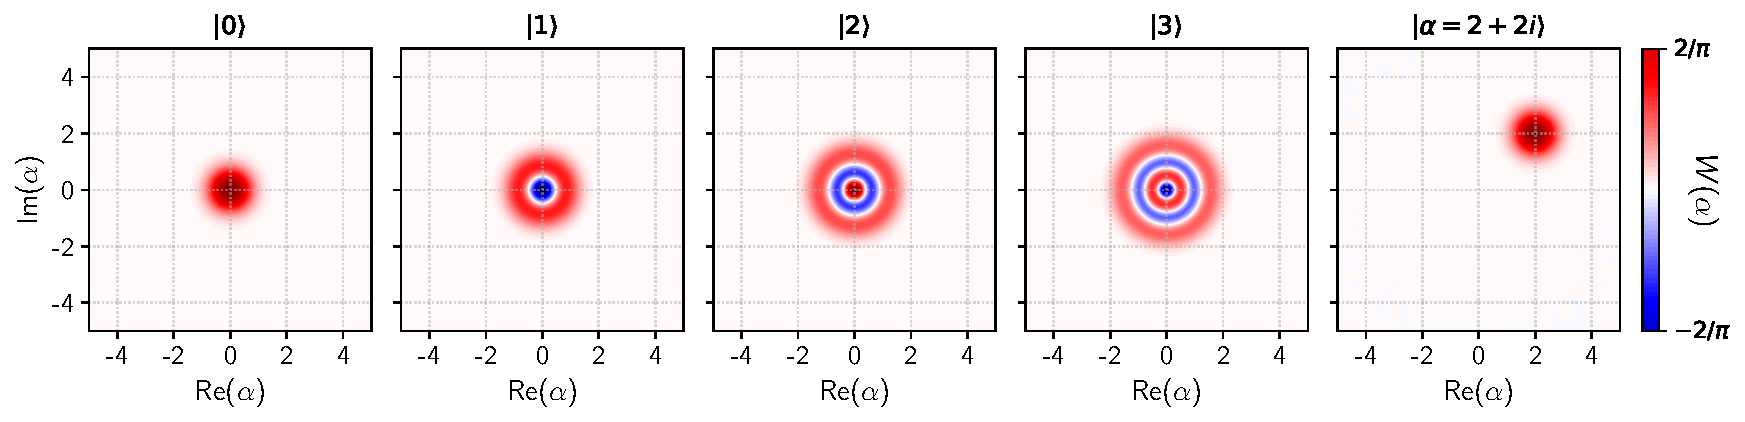
\includegraphics[width=\linewidth]{Figures/2/Fock_Wigners.pdf}
    \caption{Simulated Wigner functions for the oscillator Fock states $\ket{0}$, $\ket{1}$, $\ket{2}$, $\ket{3}$, as well as a coherent state $\ket{\alpha}$ with $\alpha = 2 + 2i$. }
    \label{fig:2_Fock_Wigners}
\end{figure}

The Wigner function has several useful mathematical properties. It integrates to unity, i.e., so that $\int W(x, p)dxdp = 1$ when expressed in terms of $x$ and $p$. Furthermore, we have marginals
\begin{equation}
    \int W(x, p)dp = |\psi(x)|^2, \qquad \int W(x, p)dx = |\psi(p)|^2
\end{equation}
and thus can also calculate position and momentum wavefunctions from the Wigner function. Lastly, using Eq. \eqref{eq:2_wigner_definition} and the definition of the characteristic function, we can rewrite $W(\alpha)$ in terms of the so-called photon number parity operator $\hat{\Pi} = (-1)^{\hat{a}^\dagger\hat{a}}$ \cite{royer1977wigner, lutterbach1997method}. After some algebra, we get
\begin{equation}
    W(\alpha) = \frac{2}{\pi}\Tr\big[\hat{D}(-\alpha)\hat{\rho}\hat{D}(\alpha)\hat{\Pi}]
\end{equation}
From this, we see that $|W(\alpha)| \leq 2/\pi$. Moreover, in practice, this gives an easy way to compute Wigner functions in circuit QED since the parity operator is something that we can quite easily measure \cite{sun2014tracking}. 


\subsection{Control, Nonlinearity, and Auxiliary Qubits\label{sec:2_control_nonlinearity_drive}}
In circuit QED, we usually control a harmonic oscillator by subjecting it to a microwave drive on one of its quadratures \cite{manenti2023quantum}. Specifically, we end up implementing a Hamiltonian of the form:
\begin{equation}
    \hat{H}(t) = \hat{H}_{\rm QHO} + \hat{H}_d(t) = \omega_a \hat{a}^\dagger \hat{a} + \epsilon(t)(\hat{a} + \hat{a}^\dagger)\cos(\omega t)
    \label{eq:2_oscillator_drive}
\end{equation}
consisting of a bare quantum harmonic oscillator (note that we have set $\h \to 1$, to equate energies and frequencies here), as well as a drive Hamiltonian $\hat{H}_d(t)$ that modulates one of the quadratures ($\hat{x} \sim \hat{a} + \hat{a}^\dagger$ in this case)\footnote{Later in our chapter on circuit QED, it will be more typical to couple to the $\hat{p} \sim i(\hat{a}^\dagger - \hat{a})$ quadrature, which corresponds to the ``charge'' of the electrical implementation of the quantum harmonic oscillator, known as an LC circuit.}. Typically, this is the only form of control that we can implement over a linear oscillator, and as we will now see, results in a displacement of the oscillator in phase space. In order to drive excitations of the system, we ideally want a resonant drive (as we did for the qubit), so that $\omega = \omega_a$. In this case, we can transform to the so-called \textbf{rotating frame} via the unitary operator $\hat{U}(t) = \exp[-i\omega t\hat{a}^\dagger \hat{a}]$ to analyze the dynamics. Since we have not yet encountered this concept in this thesis, let's now discuss it. Essentially, we can think of $\hat{U}(t)$ as a change of basis or a canonical transformation to a moving frame of reference where the quadrature axes of phase space are now themselves also rotating at frequency $\omega$. In our case, working in the ``Heisenberg picture'' of quantum mechanics at the level of operators, the effect of the time-dependent unitary $\hat{U}(t)$ is to map the Hamiltonian
\begin{equation}
    \hat{H} \mapsto \hat{U} \hat{H} \hat{U}^\dagger + i[\partial_t \hat{U}]\hat{U}^\dagger
\end{equation}
where the first term captures the change of basis and the second term is a time-dependent correction in this frame; it is analogous to, for example, a Coriolis force that arises when moving to a non-inertial frame of reference in classical mechanics \cite{goldstein-classical-mechanics}. 

Returning now to our treatment of drives in an oscillator, we can now analyze the driven QHO in the rotating frame, using the unitary $\hat{U}(t)$ to map $\hat{a} \mapsto a e^{-i\omega t}$. The new Hamiltonian reads 
\begin{equation}
    \hat{H}(t) \mapsto \hat{H}_{\rm rot}(t) = (\omega_a - \omega)\hat{a}^\dagger \hat{a} + \epsilon(t)(\hat{a} e^{-i\omega t} + \hat{a}^\dagger e^{i\omega t})\cos(\omega t)
\end{equation}
When $\omega = \omega_a$, the time-dependent correction term in this frame exactly cancels with the bare oscillator Hamiltonian $\hat{H}_{\rm QHO}$. Meanwhile, by expanding $\cos(\omega t) = (e^{i\omega t} + e^{-i\omega t})/2$, we see that the resulting drive term will have a static component and components rotating with frequencies $e^{\pm 2i\omega t}$. In the resonant case that we are considering here, these terms will be fast-oscillating and highly off resonant; we can thus often neglect them by making the famous rotating-wave approximation (RWA)\footnote{The RWA works very well in many cases, but also has its limits where the so-called counter-rotating terms at frequencies $\pm 2\omega$ cannot be ignored. We will return to the RWA many more times throughout this thesis.}. If we do this here, we are left with
\begin{equation}
    \hat{H}_{\rm rot} = \frac{\epsilon(t)}{2} \big(\hat{a} + \hat{a}^\dagger\big)
\end{equation}
where the only remaining time-dependence is the slow variation of the drive \textit{envelope} $\epsilon(t)$. If we now solve the Schr\"odinger equation $i\partial_t \ket{\psi} = \hat{H}_{\rm rot}\ket{\psi}$ with this Hamiltonian using a constant drive $\epsilon(t) = \epsilon_0$, we get the expected unitary evolution $\ket{\psi(t)} = \hat{U}_{\rm p}(t) \ket{\psi(0)}$ with the propagator given by $\hat{U}_{\rm p}(t) = \exp[-i\hat{H}_{\rm rot} t]$. We can confirm that this has the form of an oscillator displacement
\begin{equation}
    \hat{U}_{\rm p}(t) = e^{-i\epsilon_0 t(\hat{a} + \hat{a}^\dagger)/2} = \hat{D}\bigg(\frac{-i\epsilon_0 t}{2}\bigg)
\end{equation}
from which we conclude that any initial oscillator state will simply just be displaced under the action of a resonant drive. In particular, starting from the vacuum state $\ket{0}$, we have no way to prepare the Fock $\ket{1}$ state, since all higher energy levels of a linear oscillator by definition have the same frequency spacing $\omega_a$ as the $\ket{0}\to\ket{1}$ transition. Given this, it is not immediately clear how we can realize universal control and prepare nontrivial states of the oscillator for the purpose of bosonic quantum error correction.

It turns out the solution to this is to \textit{introduce} some form of nonlinearity to the otherwise linear oscillator, typically by coupling it to some auxiliary nonlinear element such as a two-level qubit/spin \cite{cai2021bosonic, raimond2006exploring, haroche2020cavity, blais2021circuit}. This approach was pioneered in cavity QED experiments in the 1990s and later adopted by circuit QED. We can get an intuitive understanding by considering the basic foundational model for coupling an oscillator to a qubit, known as the Jaynes-Cummings Hamiltonian \cite{raimond2006exploring}:
\begin{equation}
    \hat{H}_{\rm JC} = \omega_a \hat{a}^\dagger\hat{a} + \frac{\omega_q}{2}\sigmaz + g(\hat{a}^\dagger\sigmam + \hat{a}\sigmap)
\end{equation}
Here, the interaction is mediated via an operator that swaps excitations between the qubit and the oscillator. In circuit QED, we usually work in the off-resonant regime $g \ll |\omega_a - \omega_q|$; but if we briefly imagine somehow bringing the qubit into resonance with the oscillator, we are left with $g(\hat{a}^\dagger\sigmam + \hat{a}\sigmap)$ in the interaction frame. Loosely speaking, we can populate the qubit (which, due to its inherent nonlinearity, may be done using just a resonant drive), and then swap the excitation to the oscillator via the exchange interaction. If we repeat this many times, we can imagine ``climbing the ladder'' of Fock levels to to prepare nontrivial states of the joint qubit-oscillator system \cite{krause1989preparation, meystre1990cat, vogel1993quantum}. In fact, this was one of the first methods for realizing universal control over an oscillator \cite{law1996arbitrary}. 

Of course, this intuitive explanation relies on the resonant Jaynes-Cummings interaction and thus does not work in the more typical \textit{dispersive regime} where the oscillator and qubit are far-detuned with $g \ll |\omega_a - \omega_q|$. In this case, however, it is possible to approximate the Jaynes-Cummings Hamiltonian by treating the interaction as a perturbation and going to second-order in perturbation theory \cite{raimond2006exploring}. Doing this leaves with us the effective dispersive Hamiltonian
\begin{equation}
    \hat{H}_{\rm disp} = \omega_a \hat{a}^\dagger\hat{a} + \frac{\omega_q}{2}\sigmaz + \frac{\chi}{2}\hat{a}^\dagger\hat{a}\sigmaz
    \label{eq:2_dispersive_model_qubit}
\end{equation}
where the so-called \textit{dispersive shift} $\chi$ is defined here as $\chi = 2g^2/(\omega_q - \omega_a)$ and we have absorbed a Lamb shift $\omega_q \to \omega_q + g^2/(\omega_q - \omega_a)$. There is a lot to be said about Eq. \eqref{eq:2_dispersive_model_qubit}, as it is arguably the foundation on which almost all of modern circuit QED is built \cite{blais2004cavity}. The basic idea is that the effective oscillator frequency $\omega_a + \chi\sigmaz/2$ now depends on the qubit state via $\ev{\sigmaz}$, and in particular results in two different frequencies $\omega_a \pm \chi/2$ for when the qubit is in state $\ket{g}$ or $\ket{e}$ respectively. Equivalently, by regrouping the terms in Eq. \eqref{eq:2_dispersive_model_qubit} another way, the effective qubit frequency $(\omega_q + \chi \hat{a}^\dagger\hat{a})/2$ depends on the average number of photons $\ev{\hat{a}^\dagger\hat{a}}$ in the oscillator. The former grouping gives us a blueprint for the so-called \textit{dispersive readout} of a qubit, through which one may determine the qubit state just by measuring the frequency of a resonator that it is coupled to. We will return to this idea again later in this thesis, such as when we discuss circuit QED in Ch. \ref{ch:3_cQED} and when we present our experimentals in Ch. \ref{ch:4_3DGKP}. 

Finally, returning to the question of oscillator state preparation for bosonic QEC, it turns out that it is possible to achieve universal control over the joint qubit and oscillator Hilbert space just by using the dispersive interaction together with arbitrary single-qubit rotations and oscillator displacements \cite{vlastakis2015controlling, reinhold2019controlling, eickbusch2022fast}. We will discuss the specific control requirements for QEC with the GKP code in the coming sections. 

\subsection{Oscillator Error Mechanisms}

Until now, we have not yet formally discussed why oscillators may be a good platform for implementing QEC. The reason for this turns out to be that physical quantum harmonic oscillators have a particularly simple set of loss channels: single-photon loss and dephasing. In superconducting resonators, the dephasing rate $\kappa_\phi$ can be an order of magnitude smaller than the single-photon loss rate $\kappa_1$ and thus we refer to single-photon loss as the dominant error mechanism. 

At short times, the effect of photon loss can be described via a Kraus map on the density matrix $\hat{\rho}$ of the oscillator. Specifically, at short times, we can write the evolution $\hat{\rho}(t + \delta t)$ using a Kraus map
\begin{equation}
    \hat{\rho}(t + \delta t) = \mathcal{E}_{\rm loss}\big[\hat{\rho}(t)] \triangleq \sum_{\ell = 0}^\infty  \hat{E}_\ell \rho(t)  \hat{E}_\ell^\dagger
\end{equation}
where the photon loss Kraus operators $ \hat{E}_\ell$ are defined in terms of $\kappa_1$ via $\gamma = 1 - e^{-\kappa_1 \delta t}$ and have the form \cite{albert2018performance-and-structure}:
\begin{equation}
    \hat{E}_\ell = \bigg(\frac{\gamma}{1 - \gamma}\bigg)^{\ell/2} \frac{\hat{a}^\ell}{\sqrt{\ell !}} (1 - \gamma)^{\hat{n}/2}
\end{equation}
When the single-photon loss rate $\kappa_1$ or time-step $\delta t$ are small, we can approximate $\gamma \approx \kappa_1 \delta t$ and consider only:
\begin{equation}
    \hat{E}_0 \approx \hat{I} - \frac{\kappa_1 \delta t}{2}\hat{a}^\dagger\hat{a}, \quad \hat{E}_1 \approx \sqrt{\kappa_1 \delta t}\hat{a}
\end{equation}
Therefore, 
\begin{equation}
    \hat{\rho}(t + \delta t) \approx \kappa_1\delta t\bigg[\hat{a}\hat{\rho}(t)\hat{a}^\dagger - \frac{1}{2}\Big(\hat{a}^\dagger\hat{a}\hat{\rho}(t) + \hat{\rho}(t)\hat{a}^\dagger\hat{a}\Big)\bigg] + \mathcal{O}(\delta t^2)
\end{equation}
From here, we can formally write down a differential equation for the density matrix that is subject to single-photon loss. If we further include a Hamiltonian evolution $\partial_t \hat{\rho} = i[\hat{H}, \hat{\rho}]$ on top of this, we get
\begin{equation}
    \frac{d}{dt}\hat{\rho}(t) = i[\hat{H}, \hat{\rho}] + \kappa_1\mathcal{D}[\hat{a}](\hat{\rho})
    \label{eq:2_lindblad_photon_loss}
\end{equation}
where the dissipation superoperator is defined as $\mathcal{D}[\hat{a}](\cdot) = \hat{a}\cdot\hat{a}^\dagger - \frac{1}{2}\{\hat{a}^\dagger\hat{a}, \cdot\}$. We will refer to Eq. \eqref{eq:2_lindblad_photon_loss} as the Lindblad master equation, in this case for single-photon loss $\hat{a}$. For the kinds of error channels we consider in this thesis, the evolution will always take the form of a Lindblad equation, with the error operator specified by the type of loss. In particular, cavity dephasing can be described\footnote{The intuition for this is that dephasing arises from frequency fluctuations of an oscillator. Its Hamiltonian is $[\omega_0 + \delta \omega(t)]\hat{a}^\dagger\hat{a}$, which we can decompose into the bare term $\omega_0 \hat{a}^\dagger\hat{a}$ and a noisy fluctuator $\delta \omega(t)\hat{a}^\dagger\hat{a}$ that couples to the operator $\hat{a}^\dagger\hat{a}$. The same reasoning applies to qubits, whose dephasing is specified by $\sigmaz$.} by the operator $\hat{a}^\dagger\hat{a}$ and will thus result in the master equation 
\begin{equation}
    \frac{d}{dt}\hat{\rho}(t) = i[\hat{H}, \hat{\rho}] + \kappa_\phi\mathcal{D}[\hat{a}^\dagger\hat{a}](\hat{\rho})
\end{equation}
with dephasing rate $\kappa_\phi$. Moreover, later on in this chapter, we will also consider errors in a control qubit that is dispersively coupled to the oscillator via the operator $\frac{\chi}{2}\hat{a}^\dagger\hat{a}\sigmaz$. Here too, the continuous evolution of the system under the qubit loss channels can be described by:
\begin{equation}
    \frac{d}{dt}\hat{\rho}_{aq}(t) = i[\hat{H}, \hat{\rho}_{aq}] + \gamma_\downarrow\mathcal{D}[\sigmam](\hat{\rho}_{aq}) + \gamma_\uparrow\mathcal{D}[\sigmap](\hat{\rho}_{aq}) + \gamma_\phi\mathcal{D}[\sigmaz](\hat{\rho}_{aq})
\end{equation}
where now the Hamiltonian and density matrix $\hat{\rho}_{aq}$ are for the joint qubit-oscillator system. Here, we have included qubit relaxation errors at rate $\gamma_\downarrow$ via the operator $\sigmam$, excitation errors at rate $\gamma_\uparrow$ via the operator $\sigmap$, and dephasing errors at rate $\gamma_\phi = 1/T_\phi$ via the operator $\sigmaz$, which generates phase-flips. We may also define a total bit-flip rate $\gamma_1 = 1/T_1 = \gamma_\downarrow + \gamma_\uparrow$. Given that bit-flips are generated by $\sigmap$ and $\sigmam$ (or alternatively via $\sigmax$ and $\sigmay$), we might now see why bit-flip errors are particularly harmful for bosonic codes (more so than phase-flip errors). Any bosonic system with a dispersively coupled qubit and oscillator will have an interaction that is mediated via the coupling term $\hat{H}_{\rm int} = \frac{\chi}{2}\hat{a}^\dagger\hat{a}\sigmaz$. Observe that phase-flip errors commute with this interaction: $[\hat{H}_{\rm int}, \sigmaz] = 0$. Thus, a phase-flip on the qubit will, to leading order, be invisible to the oscillator. Of course, this may propagate further and cause losses, but the leading effect is that oscillators should be insensitive to such phase-flip losses. By contrast, we have $[\hat{H}_{\rm int}, \sigmap] \neq 0$ and $[\hat{H}_{\rm int}, \sigmam] \neq 0$. This means that a control qubit bit-flip \textit{can} cause backaction on the oscillator state. The specific mechanism by which this occurs will depend on the details of the bosonic code and the particular QEC protocol being used; nonetheless, it can be said that control qubit bit-flip errors are a broad problem for bosonic codes. This is what motivates us to use a bit-flip protected control qubit (heavy fluxonium) in our experiments, as we will see later in Chapters \ref{ch:4_3DGKP} and \ref{ch:5_2DGKP}. 

\clearpage
\section{A Brief Introduction to GKP Grid Codes\label{sec:2_Intro_to_GKP}}

The Gottesman-Kitaev-Preskill (GKP) grid code is a bosonic encoding that embeds a logical qubit nonlocally within the phase space of a harmonic oscillator. While the code itself has been known for two decades since the original proposal by Gottesman, Kitaev, and Preskill \cite{gottesman2001gkp} in 2001, it was only recently realized experimentally in trapped ions \cite{fluhmann2019gkp-expt, deneeve2022gkp-expt} and superconducting circuits \cite{campagne2020gkp-expt, sivak2023gkp-expt, nordquantique2023gkp-expt}. In this section, we will introduce the basic theory of the GKP code as well as its finite-energy counterpart, and then discuss the various components required for their experimental realization. 

\subsection{Ideal GKP Codes}
In general, GKP codes are defined by a lattice in the $(2N)$-dimensional phase space of $N$ quantum harmonic oscillators \cite{gottesman2001gkp, royer2022multimodegkp}. In this thesis, however, we will focus on the simplest case of a single oscillator ($N=1$) whose phase space is described by the quadrature coordinates $\hat{x}$ and $\hat{p}$ as discussed in Sec. \ref{sec:2_BosonicQEC_Definitions}. Following the original proposal of Gottesman, Kitaev, and Preskill, we can consider the square lattice with lattice constant $\ells = 2\sqrt{\pi}$ formed by the quadratures $\hat{x}$ and $\hat{p}$. The ideal GKP codewords associated with this lattice are defined as the simultaneous $+1$ eigenstates of the following two stabilizer operators: 
\begin{equation}
    \hat{S}_0^X = e^{-i\ells\hat{p}} = \hat{D}(\ell) , \qquad \hat{S}_0^Z = e^{i\ells\hat{x}} = \hat{D}(i\ell)
\end{equation}
Here, we have also defined the reduced lattice constant $\ell = \ells/\sqrt{2} = \sqrt{2\pi}$ as the \textit{phase space} displacement associated with the \textit{quadrature} (i.e., $x$ or $p$) displacement $\ell_s$. We can therefore write down the canonical GKP codewords directly. They are given by the $\hat{x}$ basis states:
\begin{equation}
    \ket{0_L} \propto \sum_{j \in \Z} \ket{x = j\ells}, \qquad \ket{1_L} \propto \sum_{j \in \Z} \ket{x = (j + 1/2)\ells}.
    \label{eq:GKP_codewords_ideal}
\end{equation}
Together, these two codewords form a two-dimensional logical subspace $\mathcal{C} \equiv \{\ket{0_L}, \ket{1_L}\}$ within the infinite-dimensional Hilbert space $\mathcal{H}$ of the oscillator. We plot wavefunctions for the codewords of Eq. \eqref{eq:GKP_codewords_ideal} in Fig. \ref{fig:2_GKP_Ideal_Wavefunctions}, which consist of a sum of Dirac delta functions. Here, we label the code states $\ket{0_L/1_L}$ as $\ket{\pm Z_L}$ instead, as a reference to the logical Bloch sphere of the GKP qubit. (We will later show Wigner functions for all six cardinal states $\ket{\pm X_L}$, $\ket{\pm Y_L}$, $\ket{\pm Z_L}$ of this Bloch sphere in the finite-energy case; see Fig. \ref{fig:2_GKP_Codewords}). However, from the ideal wavefunctions, we can already verify that the stabilizers do indeed bring the codewords back to themselves: $\hat{S}_0^X\ket{\mu_L} = \hat{S}_0^Z\ket{\mu_L} = \ket{\mu_L}$ for $\mu\in\{0, 1\}$. For $\hat{S}_0^X$, this is directly evident from Fig. \ref{fig:2_GKP_Ideal_Wavefunctions}; for $\hat{S}_0^Z$, we would need to plot the momentum wavefunction or the full Wigner function to see this. Furthermore, we also observe that logical Pauli operators can be implemented via displacements of half the lattice constant: 
\begin{figure}[t]
    \centering
    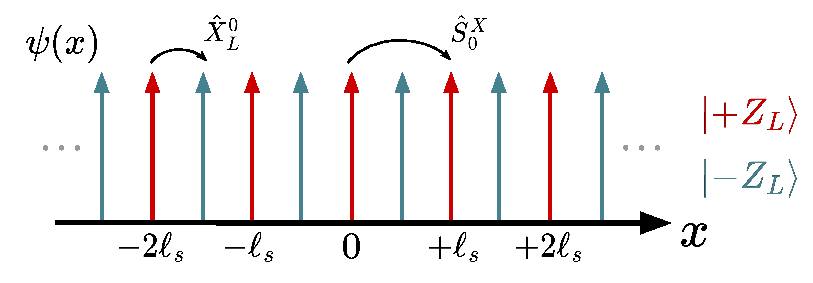
\includegraphics[width=0.85\linewidth]{Figures/2/GKP_Ideal_Wavefunctions.pdf}
    \caption{Position-basis wavefunctions for the ideal GKP codewords $\ket{0_L/1_L} = \ket{\pm Z_L}$.}
    \label{fig:2_GKP_Ideal_Wavefunctions}
\end{figure}
\begin{equation}
    \hat{X}_L^0 = \sqrt{\hat{S}_0^X} =  e^{-i\ells\hat{p}/2} , \qquad \hat{Z}_L^0 = \sqrt{\hat{S}_0^Z} = e^{i\ells\hat{x}/2}. 
\end{equation}

At this point, we might ask how the GKP states introduced above can be used for QEC. As originally proposed, the GKP code was designed to correct error channels that manifest as small phase space displacements of the oscillator: $(x, p) \to (x + \delta_x/\sqrt{2}, p+\delta_p/\sqrt{2})$. The basic principle follows from the fact that $[\hat{S}_0^Z, \hat{S}_0^X] = [e^{i\ells\hat{x}}, e^{-i\ells\hat{p}}] = 0$. Since the two GKP stabilizers commute, we can measure them simultaneously in their joint eigenbasis. This in turn implies that it is possible to measure $\hat{x}$ and $\hat{p}$ simultaneously as long as both are taken modulo $\ells/2$.\footnote{Following \cite{royer2020gkp}, we will sometimes refer to the modular quadratures $\hat{x}_{[m]} \equiv \hat{x} \Mod m$ and $\hat{p}_{[m]} \equiv \hat{p} \Mod m$ with a symmetric modulo, i.e., $\hat{x}_{[m]}, \hat{p}_{[m]} \in [-m/2, m/2)$. We are specifically interested in $\hat{x}_{[\ells/2]}$ and $\hat{p}_{[\ells/2]}$.} Therefore, if a displacement error shifts the GKP grid by an amount $(x, p) \to (x + \delta_x/\sqrt{2}, p+\delta_p/\sqrt{2})$, we can simply measure the modular quadratures and then apply a correction operation $\hat{D}(-\alpha)$ with $\alpha = \delta_x + i\delta_p$ to re-center the grid. If the errors are small, i.e., $|\delta_x|, |\delta_p| < \ell / 4$ (now expressed in terms of the \textit{phase space} grid), this results in a perfect recovery of the logical information. We depict this process in Fig. \ref{fig:2-GKP-Ideal-QEC}(a) showing the effect of a displacement error on the full Wigner function of the code (which, as expected, has the form of a 2D grid in phase space). Now, it turns out that for realistic oscillators, most physical decoherence processes such as single-photon loss or dephasing occur via a continuous distortion of phase space. This means that these error mechanisms can be corrected by the GKP code if the GKP stabilizers are measured frequently enough \cite{gottesman2001gkp, glancy2006gkperror, albert2018performance-and-structure, noh2018performance-and-structure-pt2}. Among the various single-mode bosonic codes, it was recently shown that the GKP code offers the best protection against photon loss, which is the dominant error mechanism for superconducting resonators \cite{albert2018performance-and-structure}. 
\begin{figure}[h]
    \centering
    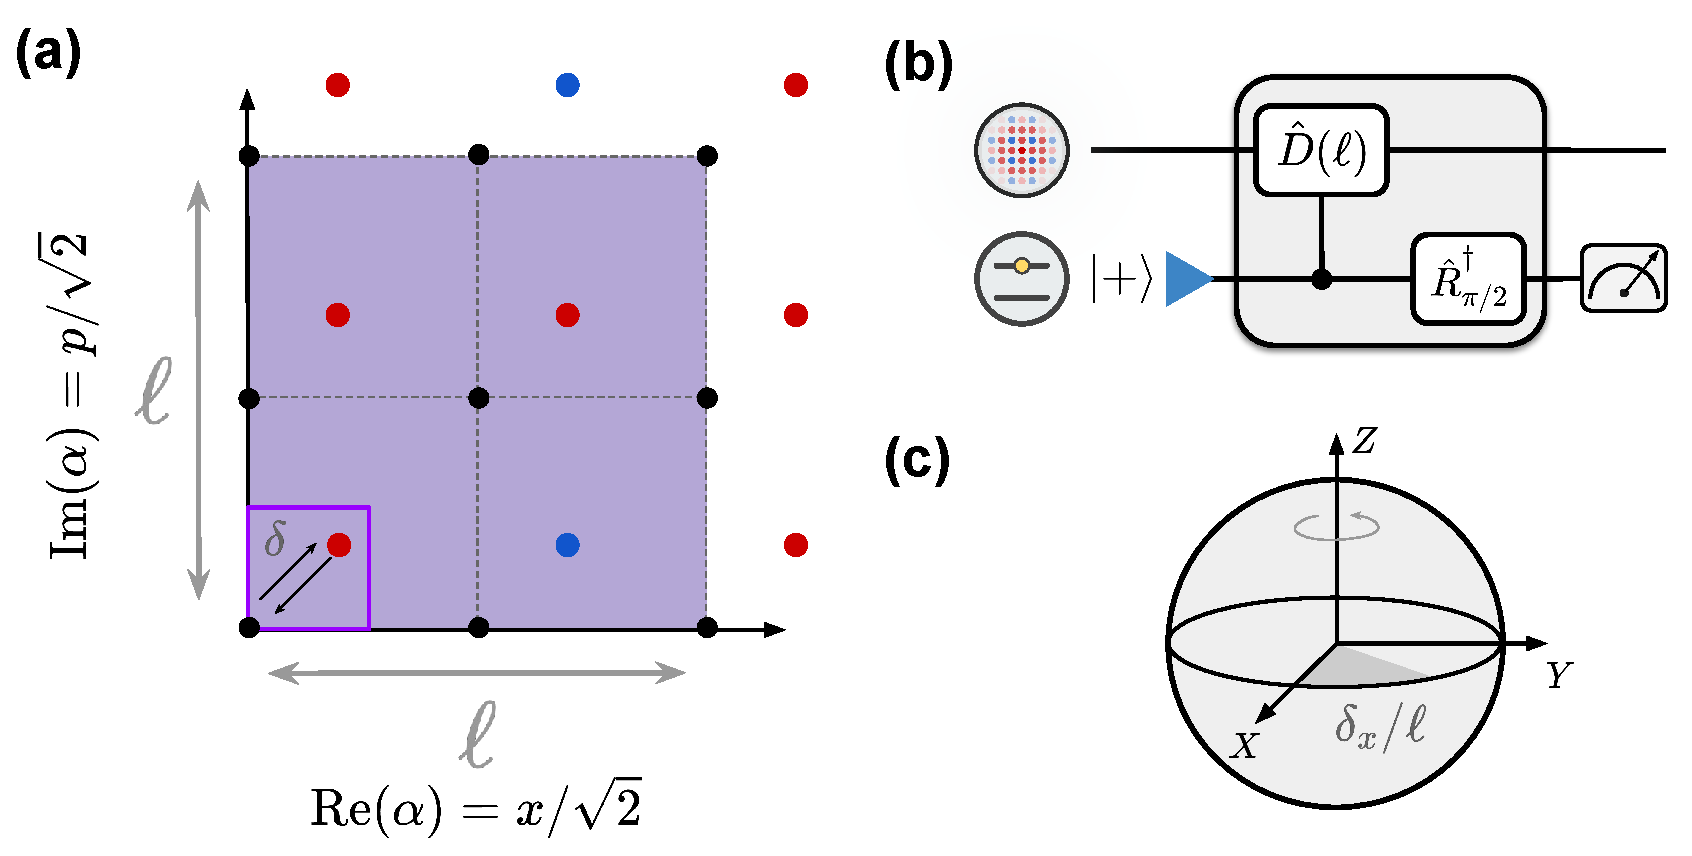
\includegraphics[width=0.85\linewidth]{Figures/2/GKP Ideal QEC.pdf}
    \caption[Schematic for ideal GKP error correction using phase estimation on an auxiliary qubit.]{\textbf{(a)} Wigner function for GKP $|0_L\rangle$ state under the effect of a small displacement $\delta = \delta_x + i\delta_p$. We plot the Wigner in phase space coordinates ${\rm Re}(\alpha)$ and ${\rm Im}(\alpha)$. If the error is small $|\delta_x|, |\delta_p| < \ell / 4$ (purple box), we can correct the error exactly. \textbf{(b,c)} Stabilizer circuit for GKP QEC which uses a conditional displacement to map error information to the phase of a control qubit. We plot this phase along the equator of the control qubit Bloch sphere.}
    \label{fig:2-GKP-Ideal-QEC}
\end{figure}

For an ideal GKP code, the actual stabilizer measurements can be carried out by using an auxiliary qubit as shown in Fig. \ref{fig:2-GKP-Ideal-QEC}(b). This QEC circuit maps the stabilizer information onto the phase of the qubit using a conditional displacement operation
\begin{equation}
    {\rm CD}(\ell) = \hat{D}\bigg(\frac{+\ell}{2}\bigg)\op{g}{g} + \hat{D}\bigg(\frac{-\ell}{2}\bigg)\op{e}{e} = \exp[\ell(\hat{a}^\dagger - \hat{a}) \sigmaz / 2].
    \label{eq:2_CD_unitary_definition}
\end{equation}
From the perspective of the oscillator, the CD gate implements a displacement conditioned on the state of the qubit; meanwhile, from the perspective of the qubit, this same operation can be seen as a rotation about the $z$-axis of the Bloch sphere by an amount $\ev{\hat{a}^\dagger - \hat{a}}\ell/2$. If the oscillator has suffered a displacement by $\delta = \delta_x + i\delta_p$, the circuit in Fig. \ref{fig:2-GKP-Ideal-QEC}(b) has the the effect of imparting a phase proportional to $\delta_x/\ell$ onto the qubit. By then measuring the qubit, we can use a one-bit phase estimation to determine $\delta_x$ bit-by-bit; we then perform intermediate small displacements to continuously correct this over many rounds of repeated stabilizer measurements \cite{terhal2016phase-estimation, terhal2020bosonic}. We of course must also interleave this with conditional displacements along the other quadrature $i\ell$ to extract the error $\delta_p$. Intuitively, however, we can think of this QEC process as continuously measuring the quadratures $x$ and $p$ modulo $\ells$ and applying feedback displacements to correct the small displacement errors that arise. 

\clearpage

\subsection{Finite-Energy GKP Codes}

While the ideal GKP codewords $\ket{\mu_L}$ make clear how the grid code can be used for error correction, it remains to be seen how to realize them in practice. On their own, the states $\ket{\mu_L}$ are non-normalizable superpositions of infinitely squeezed states that extend across the entire phase space of the oscillator; they contain infinite energy and so cannot actually be realized in the lab. Moreover, for realistic systems with loss such as those we encounter in cQED, it is simply not feasible to have an arbitrarily large energy state in the oscillator. The reason for this is that the rates of various physical error channels scale with the number of photons/excitations. For example, amplitude damping where the photon loss rate $\Gamma_n$ with which the Fock state $\ket{n}$ decays to $\ket{n-1}$ scales as $\Gamma_n = n\Gamma_1$, where $\Gamma_1$ is the single-photon loss rate. Another example is the Kerr nonlinearity that a resonator inherits from its coupling to a nonlinear auxiliary control element (this will be discussed in Chapter \ref{ch:3_cQED}). To remedy the situation, it is necessary to bound the squeezing of the GKP states and limit their extent in phase space. Furthermore, one must design error correction strategies that maintain the oscillator photon number so that such errors do not accumulate over time \cite{campagne2020gkp-expt}. We can realize physical, finite-energy GKP states by applying an envelope operator $\hat{E}_\Delta$ to the codewords \cite{royer2020gkp}. A natural choice is a Gaussian envelope $\hat{E}_\Delta = \exp(-\Delta^2 \hat{a}^\dagger\hat{a})$, which gives the individual peaks of the GKP states a finite width $\Delta$ while also applying an overall Gaussian envelope of width $1/\Delta$ to the entire grid. We define the finite-energy GKP codewords as 
\begin{equation}
    \ket{\tilde{\mu}_L} = \mathcal{N}_\Delta \hat{E}_\Delta \ket{\mu_L}
\end{equation}
for $\mu \in \{0, 1\}$, where $\mathcal{N}_\Delta$ is a normalization factor. These approximate GKP states $\ket{\tilde{\mu}_L}$ are non-orthogonal for non-zero $\Delta$, and are also no longer eigenstates of the ideal stabilizers $\hat{S}_0^{X/Z}$. However, it turns out that it is still possible to define exact stabilizers for the finite-energy code
\begin{equation}
    \hat{S}_\Delta^{X/Z} = \hat{E}_\Delta\,\hat{S}_0^{X/Z}\,\hat{E}_\Delta^{-1}
\end{equation}
which, by construction, satisfy $\hat{S}_\Delta^{X/Z}\ket{\tilde{\mu}_L} = \ket{\tilde{\mu}_L}$. We can similarly define regularized logical Pauli operators $\hat{X}_L^\Delta = \hat{E}_\Delta \hat{X}_L^0 \hat{E}_\Delta^{-1}$ and $\hat{Z}_L^\Delta = \hat{E}_\Delta \hat{Z}_L^0 \hat{E}_\Delta^{-1}$ via the same transformation. Clearly, as $\Delta \to 0$, the finite-energy GKP states and operators will approach their ideal infinite-energy counterparts, albeit at the expense of a higher average photon number in the codewords 
\begin{equation}
    \bar{n}_{\rm GKP} = \frac{1}{2} \sum_{\mu\in \{0,1\}} \mel{\tilde{\mu}_L}{\hat{a}^\dagger\hat{a}}{\tilde{\mu}_L} \approx \frac{1}{2\Delta^2} - \frac{1}{2}
\end{equation}
and the detrimental effects that come with it. Conversely, increasing $\Delta$ too much results in a non-negligible loss in fidelity due to the increasing finite overlap $\ip{\tilde{0}_L}{\tilde{1}_L}$, and in general reduces the code's ability to correct errors \cite{royer2020gkp}. We can therefore view $\Delta$ as a controllable parameter which determines the `size' of the GKP code, and whose value can be optimized in experiment. 

%\footnote{For realistic resonators in circuit QED with significant single-photon loss, it is often best to use a low number of oscillator photons (e.g. $\bar{n}_{\rm GKP} \lesssim 5$). Recent GKP experiments in Refs. \cite{sivak2023gkp-expt} and \cite{nordquantique2023gkp-expt} used $\Delta = 0.34$ and $\Delta = 0.36$ respectively, corresponding to roughly 3-4 photons. As the quality of resonators improves, so too will this tradeoff.}.


\begin{figure}[h]
    \centering
    \includegraphics[width=\linewidth]{Figures/2/GKP_Wigners_Delta.pdf}
    \caption[Simulated Wigner functions for the finite-energy GKP codewords $\ket{\tilde{0}_L}$/$\ket{\tilde{1}_L}$ as a function of the GKP finite-energy width parameter $\Delta$]{Simulated Wigner functions for the finite-energy GKP codewords $\ket{\tilde{0}_L}$/$\ket{\tilde{1}_L}$ as a function of the parameter $\Delta$, which sets the width of the individual peaks as well as the overall extent of the grid in phase space via $1/\Delta$. The associated mean photon numbers $n_{\rm GKP}$ are approximately 200, 22, 7.5, and 3.6, respectively, as $\Delta$ increases.}
    \label{fig:2_GKP_Wigners_Delta}
\end{figure}

\begin{figure}
    \centering
    \includegraphics[width=0.8\linewidth]{Figures/2/GKP_Codewords.pdf}
    \caption[Simulated Wigner functions and associated wavefunctions for the six cardinal states of the logical GKP Bloch sphere:$\ket{\pm \tilde{Z}_L}$, $\ket{\pm \tilde{X}_L}$, $\ket{\pm \tilde{Y}_L}$.]{Simulated Wigner functions and associated wavefunctions for the six cardinal states of the logical GKP Bloch sphere: \textbf{(a)} $\ket{\pm \tilde{Z}_L}$, \textbf{(b)} $\ket{\pm \tilde{X}_L}$, and \textbf{(c)} $\ket{\pm \tilde{Y}_L}$. Here we have chosen the finite-energy envelope $\Delta = 0.2$, and we plot Wigners vs. the quadratures $(x, p)$.}
    \label{fig:2_GKP_Codewords}
\end{figure}
\clearpage

\section{Open-Loop GKP Error Correction \label{sec:2_OpenLoopGKPQEC}}

In circuit QED, there are various approach one could take to simply \textit{prepare} GKP states, e.g. via optimal control protocols such as GRAPE \cite{khaneja2005grape, reinhold2019thesis}, SNAP \cite{krastanov2015-SNAP, heeres2015-SNAP, fosel2020-SNAP}, or ECD \cite{eickbusch2022fast}; via periodic (Floquet) driving in a SQUID \cite{gkp-periodic-drive2024}; or by engineering superconducting circuits with GKP-like ground states \cite{rymarz2021hardwaregkp}. However, we are generally more interested in protocols that prepare \textit{and} continuously stabilize GKP states via stabilizer measurements and active error correction. For ideal GKP codewords, we saw how to do this with phase estimation in Fig. \ref{fig:2-GKP-Ideal-QEC}. On the other hand, for realistic GKP codewords in practice, we need to measure the corresponding stabilizers $\hat{S}_\Delta^{X/Z}$ instead. It turns that this is possible to do by modifying the circuit in Fig. \ref{fig:2-GKP-Ideal-QEC} to account for the finite-energy envelope \cite{fluhmann2019gkp-expt, campagne2020gkp-expt, royer2020gkp, deneeve2022gkp-expt}; furthermore, QEC can be realized ``autonomously'' by replacing the measurement-based feedback step with an unconditional qubit reset. More precisely, we refer to this as \textit{open-loop} error correction (in the language of control theory) to distinguish it from QEC based on feedback control. To arrive at this result, it ends up being helpful to take a different view of the QEC process as a form of engineered dissipation \cite{royer2020gkp, vlad2023thesis}. In this picture, errors can be described as excitations out of the GKP code manifold; error correction then entails realizing a dissipative quantum channel to `cool' these excitations and stabilize the code space. Following the theoretical treatment in Ref. \cite{royer2020gkp}, the desired dissipation channel on the oscillator can be decomposed as an interaction between the oscillator and an auxiliary qubit that is reset after each round of cooling (error correction), i.e., effectively transferring entropy out of the system. We refer the reader to Refs. \cite{royer2020gkp, sivak2023gkp-expt, vlad2023thesis} for a rigorous derivation and discussion of this theory\footnote{We also point out Refs. \cite{sellem2023gkp, sellem2024gkp} which introduce an entirely different dissipation channel for the GKP code, though the main idea there is also to autonomously stabilize the code space albeit with more dissipators.}, and here instead just convey the main result. Based on different Trotter decompositions of the generalized dissipation channel in \cite{royer2020gkp}, there are actually several candidate qubit-oscillator circuits/protocols that can realize open-loop QEC of the finite-energy GKP code. In this thesis, we work primarily with the Small-Big-Small (SBS) protocol\footnote{The other two protocols are called Sharpen-Trim (ST) and Big-Small-Big (BSB). Both require two large CD gates, and ST also has two reset steps. Meanwhile SBS requires just one of each (see next section).}, shown below. 
\begin{figure}[h]
    \centering
    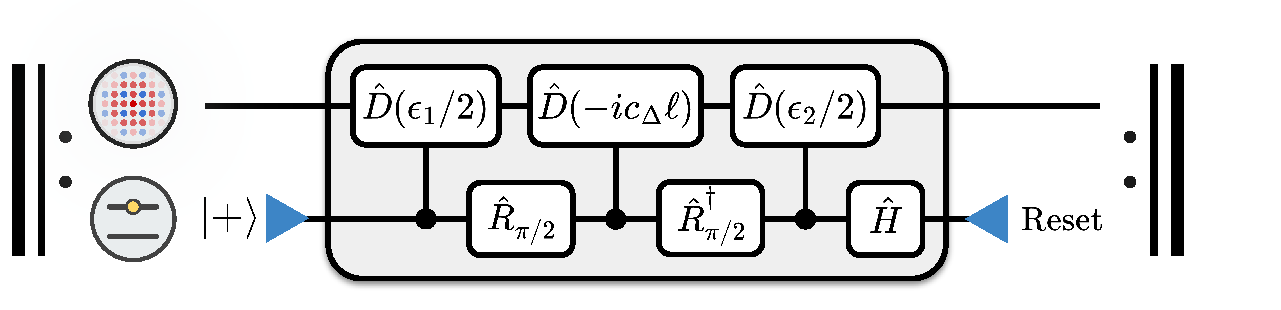
\includegraphics[width=0.83\linewidth]{Figures/2/SBS.pdf}
    \caption[Gate sequence for the Small-Big-Small (SBS) open-loop GKP error correction protocol.]{Gate sequence for the Small-Big-Small (SBS) error correction protocol, which consists of interleaved qubit rotations and oscillator conditional displacements, followed by qubit reset. QEC is implemented via repeated application of this sequence and its complement (the latter having displacements $\beta \to i\beta$ on all CDs). See text for details.}
    \label{fig:2-SBS}
\end{figure}

\subsection{The Small-Big-Small (SBS) Protocol\label{sec:2_SBS}}
\textbf{Overview.} The SBS circuit consists of 3 conditional displacement (CD) gates interleaved by qubit rotations; the relative magnitudes of the CDs motivate the name Small-Big-Small. The middle CD is a phase space displacement of magnitude $c_\Delta \ell \approx \ell$; it effectively realizes phase estimation to measure the GKP stabilizer. Here $c_\Delta \equiv \cosh(\Delta^2)$, and we note that $c_\Delta \approx 1$ for all practical values ($\Delta \lesssim 0.4$) of the GKP size. The first and last CD operations are small corrections that account for the finite-energy envelope and perform autonomous error correction respectively (see e.g. \href{https://youtu.be/TOQzHkgsH_E?t=1045}{this talk}). From theory, we expect $\epsilon_1 = \epsilon_2 = s_\Delta \ell$ with $s_\Delta \equiv \sinh(\Delta^2) \approx \Delta^2$. However, in Ref. \cite{sivak2023gkp-expt}, the authors optimized the two small displacements independently and found, through use of a reinforcement learning (RL) agent, that choosing $\epsilon_2 \gtrsim \epsilon_1$ gave the best QEC performance. This observation has since been corroborated in simulation when accounting for all error channels acting during the SBS unitary, and was also reported in another experiment \cite{nordquantique2023gkp-expt}. Essentially, although $\epsilon_1 = \epsilon_2$ holds for a lossless circuit, when including loss the optimal ratio $\epsilon_2/\epsilon_1$ turns out to be strongly dependent on the actual error channels involved, and is thus another free parameter (like $\Delta$) that can be tweaked in experiment to get the best QEC gain. Finally, it is important to note that the circuit above carries out phase estimation for the $\hat{S}_\Delta^{Z}$ stabilizer; to get the circuit for the $\hat{S}_\Delta^{X}$ stabilizer, we just map ${\rm CD}(\beta) \to {\rm CD}(i\beta)$. The full QEC sequence for SBS then involves repeatedly alternating between the two circuits to stabilize both quadratures. 

\noindent \textbf{Kraus Operators for SBS.} We can describe the SBS protocol in a more quantitative manner by considering it as a quantum channel. To this end, let us imagine that the SBS reset step is implemented using measurement-based active reset. In this case, although the oscillator QEC is still `autonomous', we would have access to the error syndromes by looking at the measurement statistics of the qubit. A subtle yet interesting feature of the circuit above is that---in the absence of errors---it leaves the qubit and oscillator completely disentangled after the unitary evolution (gray box in Fig. \ref{fig:2-SBS}). Thus, if no error occurs, the qubit state will end up in $\ket{g}$ before reset. In our current measurement-based reset approach, then, a measurement outcome $\ket{g}$ would signify ``no error'' while a measurement outcome $\ket{e}$ would imply that an error was detected and corrected. Based on these two outcomes, we can write down the action of the SBS circuit above on just the oscillator by evolving a full qubit-oscillator state through the circuit and then finally tracing out the qubit. This leaves us with a pair of Kraus operators $\hat{K}_g^Z, \hat{K}_e^Z$ for the oscillator, which are given by\footnote{I owe a huge thanks to Jonathan Pelletier for his help deriving these expressions for the general case $\epsilon_1 \neq \epsilon_2$.}:     
\begin{align}
    \begin{split}
        \hat{K}_g^Z &= \cos\bigg(\frac{\epsilon_2 \sqrt{\pi}}{2\sqrt{2}}\bigg)\Bigg[\cos\bigg(\frac{\epsilon_2 + \epsilon_1}{2\sqrt{2}} \hat{p}\bigg)\cos(\sqrt{\pi} \hat{x}) + i\sin\bigg(\frac{\epsilon_2 - \epsilon_1}{2\sqrt{2}} \hat{p}\bigg)\sin(\sqrt{\pi} \hat{x})\Bigg] \\
        &\quad + \sin\bigg(\frac{\epsilon_2 \sqrt{\pi}}{2\sqrt{2}}\bigg)\Bigg[\cos\bigg(\frac{\epsilon_2 - \epsilon_1}{2\sqrt{2}} \hat{p}\bigg)\cos(\sqrt{\pi} \hat{x}) - i\sin\bigg(\frac{\epsilon_2 + \epsilon_1}{2\sqrt{2}} \hat{p}\bigg)\sin(\sqrt{\pi} \hat{x})\Bigg]
    \end{split} \\
    \begin{split}
        \hat{K}_e^Z &= -\cos\bigg(\frac{\epsilon_2 \sqrt{\pi}}{2\sqrt{2}}\bigg)\Bigg[i\sin\bigg(\frac{\epsilon_2 + \epsilon_1}{2\sqrt{2}} \hat{p}\bigg)\cos(\sqrt{\pi} \hat{x}) + \cos\bigg(\frac{\epsilon_2 - \epsilon_1}{2\sqrt{2}} \hat{p}\bigg)\sin(\sqrt{\pi} \hat{x})\Bigg] \\
        &\quad -\sin\bigg(\frac{\epsilon_2 \sqrt{\pi}}{2\sqrt{2}}\bigg)\Bigg[i\sin\bigg(\frac{\epsilon_2 - \epsilon_1}{2\sqrt{2}} \hat{p}\bigg)\cos(\sqrt{\pi} \hat{x}) - \cos\bigg(\frac{\epsilon_2 + \epsilon_1}{2\sqrt{2}} \hat{p}\bigg)\sin(\sqrt{\pi} \hat{x})\Bigg]
    \end{split}
\end{align}
For an input state $\hat{\rho}\otimes \op{+}{+}$ to the SBS circuit, the oscillator state $\hat{\rho}$ after unitary evolution and reset is given by
\begin{equation}
    \hat{\rho} \mapsto \mathcal{R}_\Delta^Z(\hat{\rho}) = \hat{K}_g^Z \hat{\rho} \hat{K}_g^Z{}^\dagger + \hat{K}_e^Z \hat{\rho} \hat{K}_e^Z{}^\dagger  
\end{equation}
where $\mathcal{R}_\Delta^Z$ is the rank-2 dissipator towards the $+1$ eigenspace of $\hat{S}_\Delta^Z$. To get the equivalent dissipator $\mathcal{R}_\Delta^X$ for the stabilizer $\hat{S}_\Delta^X$, we can map $\hat{K}_{g/e}^Z \to \hat{K}_{g/e}^X$ by making the replacement $(x, p) \to (p, -x)$. Finally, the quantum channel for the full SBS QEC cycle is $\mathcal{R}_\Delta = \mathcal{R}_\Delta^X \circ \mathcal{R}_\Delta^Z$. 

In practice, we envision in our experiments using a fully unconditional qubit reset rather than measurement-based feedback. In this case, we won't have access to the measurement statistics (i.e., the protocol will be truly \textit{open-loop}). Furthermore, the final qubit Hadamard gate can be omitted from the protocol and absorbed into the reset operation. Nonetheless, for theoretical analysis and certain numerical simulations, it will make things considerably easier to continue working in the artificial measurement-based feedback picture using the Kraus operators for SBS.

\noindent\textbf{Logical Pauli Measurements.} Quantum error correction with the SBS protocol consists of multiple rounds of the circuit from Fig. \ref{fig:2-SBS}, which we saw can be expressed as a quantum channel for the oscillator state in terms of the Kraus operators $\hat{K}_{g/e}^{Z}$ and $\hat{K}_{g/e}^{X}$ above. It will also turn out to be useful to define similar operations to describe logical \textit{measurements}, i.e., measuring $\hat{X}_L^\Delta$, $\hat{Y}_L^\Delta$, and $\hat{Z}_L^\Delta$ within the GKP codespace. These are also derived in Ref. \cite{royer2020gkp} and can be expressed as follows. To measure $\hat{X}_L^\Delta$, $\hat{Y}_L^\Delta$, or $\hat{Z}_L^\Delta$ respectively for a given joint qubit-oscillator state $\hat{\rho}_{aq}$, we first apply one of three unitaries $\hat{M}_x$, $\hat{M}_y$, or $\hat{M}_z$ and then measure the qubit in the $z$-basis. The operators are defined in terms of $\epsilon = s_\Delta \ells$ as follows:
\begin{align}
    \begin{split}
        \hat{M}_x &= e^{-i\ell_s c_\Delta \hat{p}\sigmax / 4} e^{i \epsilon \hat{x}\sigmay/4} \\
        \hat{M}_y &= e^{-i\ell_s c_\Delta (\hat{x}+\hat{p})\sigmax / 4} e^{i \epsilon (\hat{x}-\hat{p})\sigmay/4} \\
        \hat{M}_z &= e^{-i\ell_s c_\Delta \hat{x}\sigmax / 4} e^{-i \epsilon \hat{p}\sigmay/4}
    \end{split}
\end{align}
To see an example of this in practice, we demonstrate a numerical simulation of SBS QEC in Fig. \ref{fig:2_SBS_NoLoss_QEC_Sim} below. Here, we consider the case of no error channels  and thus starting from an initial oscillator state $\hat{\rho}_0$ each round of SBS can be described via the application of the two QEC channels
\begin{equation}
    \hat{\rho}_{i + 1} = (\mathcal{R}_\Delta^X \circ \mathcal{R}_\Delta^Z)(\hat{\rho}_i) = \mathcal{R}_\Delta^X\Big[\mathcal{R}_\Delta^Z(\hat{\rho}_i)\Big]
\end{equation}
i.e., each QEC round consists of stabilizing both $X$ and $Z$. We start from the vacuum state $\hat{\rho}_0 = \op{0}{0}$ in the oscillator and perform 30 rounds of SBS (15 rounds of QEC). Over time, we see the the oscillator converges towards the GKP code manifold, and after 30 rounds the oscillator state is approximately $\hat{\rho} \approx \frac{1}{2}\op{+\tilde{Z}_L}{+\tilde{Z}_L} + \frac{1}{2}\op{+\tilde{X}_L}{+\tilde{X}_L}$. This is because our initial vacuum state $\ket{0}$ has support over both even parity GKP cardinal states $+X_L$/+$Z_L$. 

After round 30, we perform a projective measurement of $\hat{Z}_L^\Delta$ within the codespace via the operator $\hat{M}_z$. This involves first mapping the oscillator state $\hat{\rho} \mapsto \hat{\rho}_{aq} = \hat{M}_z(\hat{\rho}\otimes \op{g}{g})\hat{M}_z^\dagger$, and then projecting onto the measurement outcome of measuring $\ket{g}$ in the qubit, which is done using the projector $\hat{I}_a \otimes \op{g}{g}$. Specifically, we map $\hat{\rho}_{aq} \mapsto (\hat{I}_a \otimes \op{g}{g}) \hat{\rho}_{aq}(\hat{I}_a \otimes \op{g}{g})$, normalize, and then trace out the qubit to get an oscillator-only state $\hat{\rho}_z$ after measurement. Choosing the outcome $\ket{g}$ results in this final oscillator state $\hat{\rho}_z \approx \ket{+\tilde{Z}_L}$; if we had chosen $\ket{e}$, we would end up with a state close to $\ket{-\tilde{Z}_L}$. After the measurement, we continue stabilizing with 30 more rounds of SBS, which brings us closer to the true codeword $\hat{\rho} \to \ket{+\tilde{Z}_L}$. We plot this entire process in Fig. \ref{fig:2_SBS_NoLoss_QEC_Sim} showing the expectation value $\ev{\hat{Z}_L^\Delta}$ as a function of time, as well as the oscillator Wigner functions for (i) the initial state $\hat{\rho}_0$, (ii) the state before measurement, and (iii) the final state $\approx \ket{+Z_L^\Delta}$. 

\begin{figure}[h]
    \centering
    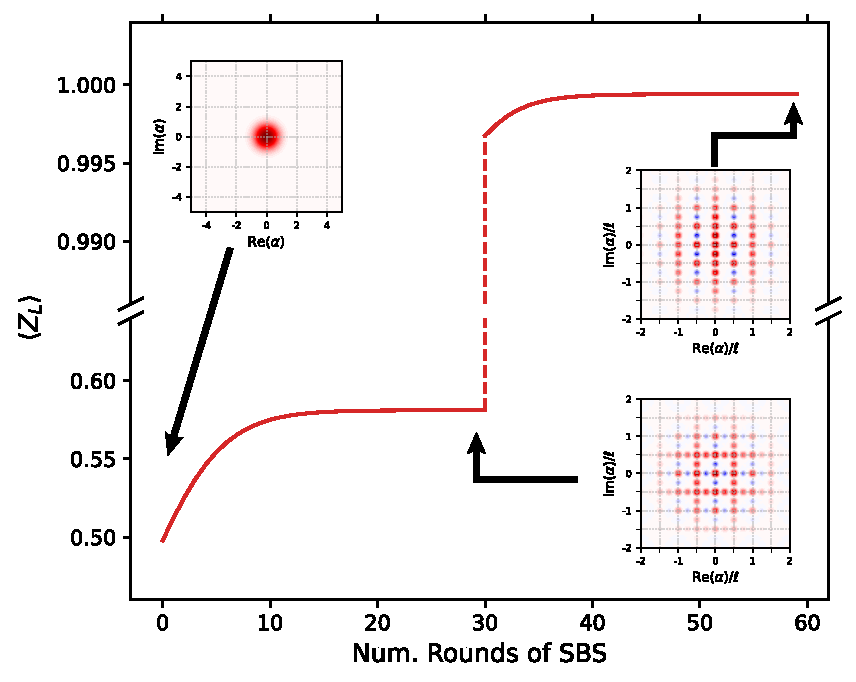
\includegraphics[width=0.85\linewidth]{Figures/2/SBS_NoLoss_QEC_Sim.pdf}
    \caption[Simulated SBS stabilization of the GKP $\ket{+\tilde{Z}_L}$ state for a lossless oscillator.]{Plot of expectation value $\ev{\hat{Z}_L^\Delta}$ vs. time over multiple rounds of SBS. We see the oscillator state converge to the GKP code manifold over 30 rounds of SBS. At round 30, we perform a logical projective measurement of $\hat{Z}_L^\Delta$, and then continue with 30 additional rounds of SBS. The oscillator state converges to the codeword $\hat{\rho} \to \ket{+\tilde{Z}_L}$ as shown by the final Wigner function. We also plot the Wigner functions for the initial vacuum state and the intermediate state before the logical measurement. Note $\Delta = 0.25$ and $\epsilon_1 = \epsilon_2$ here.}
    \label{fig:2_SBS_NoLoss_QEC_Sim}
\end{figure}

\subsection{SBS with Oscillator Single-Photon Loss}
Following up from the ideal stabilization case in Fig. \ref{fig:2_SBS_NoLoss_QEC_Sim} above, we can also examine what happens during SBS error correction when there is single-photon loss on the oscillator. In this case, we define \begin{equation}
    \hat{\rho}_{i + 1} =  \mathcal{E}_{\rm loss}\Big(\mathcal{R}_\Delta^X\Big[\mathcal{E}_{\rm loss}\Big(\mathcal{R}_\Delta^Z(\hat{\rho}_i)\Big)\Big]\Big)
    \label{eq:2_SBS_Lossy_Kraus}
\end{equation}
i.e., we interleave the single-photon loss channel $\mathcal{E}_{\rm loss}$ with the error correction channels. We demonstrate an example of evolving an oscillator vacuum state $\ket{0}$ under this equation in Fig. \ref{fig:2_SBS_Lossy_QEC_Sim}, setting $\Delta = 0.25$ and $\epsilon_1 = \epsilon_2$ for the GKP code and $\kappa_1\delta t = 8\times 10^{-3}$ for the loss.
\begin{figure}[h]
    \centering
    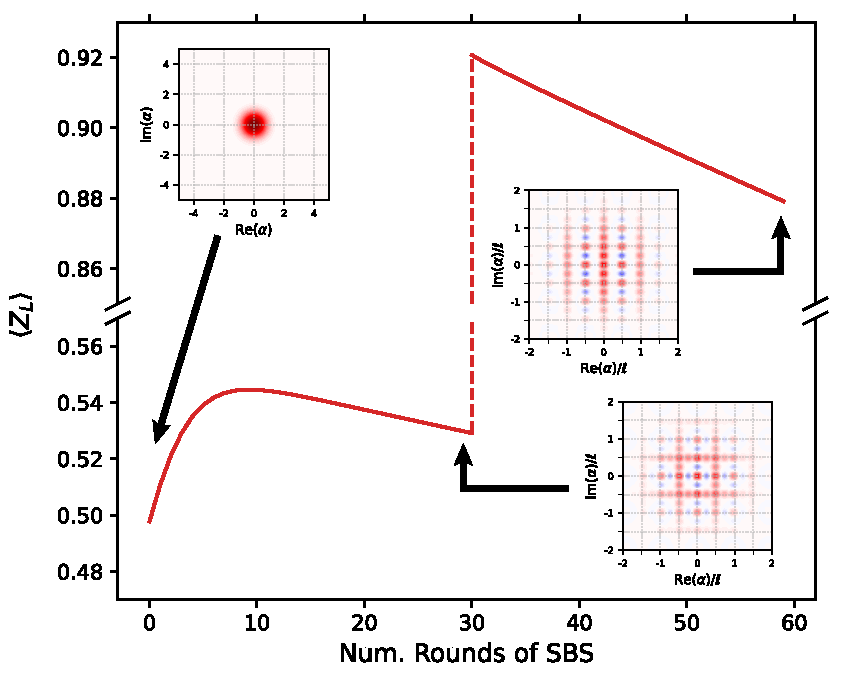
\includegraphics[width=0.85\linewidth]{Figures/2/SBS_Lossy_QEC_Sim.pdf}
    \caption[Simulated SBS stabilization of the GKP $\ket{+\tilde{Z}_L}$ state for an oscillator with single-photon loss.]{Plot of expectation value $\ev{\hat{Z}_L^\Delta}$ vs. time over multiple rounds of SBS. We take $\Delta = 0.25$ and $\epsilon_1 = \epsilon_2$ for the GKP code, and set $\kappa_1\delta t = 8\times 10^{-3}$. Starting from the vacuum state, we first converge to the codespace over 30 rounds, perform a logical measurement of $\hat{Z}_L^\Delta$, and then stabilize for another 30 rounds. Due to the single-photon loss, we see $\ev{\hat{Z}_L^\Delta}$ decay exponentially with time. Compared to Fig. \ref{fig:2_SBS_NoLoss_QEC_Sim}, the contrast of the Wigner functions is also reduced here due to the effect of the loss on the stabilization.}
    \label{fig:2_SBS_Lossy_QEC_Sim}
\end{figure}

Note that the single-photon loss channel $\mathcal{E}_{\rm loss}$ is entirely specified in terms of the product $\kappa_1\delta t$, where $\delta t$ is a period over which we accrue loss. The evolution modelled by Eq. \eqref{eq:2_SBS_Lossy_Kraus} is thus one of instantaneous QEC channels interleaved by periods $\delta t$ of photon loss, which is meant to approximate the true error correction process occurring continuously over the period $\delta t$. One could also perform a full master equation simulation [cf. Eq. \eqref{eq:2_lindblad_photon_loss}] of the SBS gate sequence in Fig. \ref{fig:2-SBS}, but this will give similar results for small $k_1\delta t$. 

The SBS evolution shown here in Fig. \ref{fig:2_SBS_Lossy_QEC_Sim} is only meant to be an illustrative example of the GKP error correction process, showing what happens when QEC and single-photon loss both occur simultaneously. We will demonstrate more extensive such simulations in Ch. \ref{ch:5_2DGKP}, where we sweep over various amounts of single-photon loss $\kappa_1\delta t$. In those simulations, we will actually fit the exponential decay of $\ev{\hat{Z}_L^\Delta}$ with time to extract the lifetime $T_{\ket{+Z}}$ for the state $\ket{+\tilde{Z}_L}$. To give a preview, in the simulation we show in Ch. \ref{ch:5_2DGKP}, we will then repeat this QEC process to prepare all six cardinal states $\ket{\pm \tilde{Z}_L}$, $\ket{\pm \tilde{X}_L}$, $\ket{\pm \tilde{Y}_L}$ of the GKP logical Bloch sphere. From there, we can calculate $T_Z = \frac{1}{2}[T_{\ket{+Z}} + T_{\ket{-Z}}]$, and likewise for $X$ and $Y$, to finally get
\begin{equation}
    T_L = 3\bigg(\frac{1}{T_X} + \frac{1}{T_Y} + \frac{1}{T_Z}\bigg)^{-1}
\end{equation}
as the total logical lifetime of the GKP qubit averaged over all six cardinal states \cite{royer2020gkp, sivak2023gkp-expt}. In Ch. \ref{ch:5_2DGKP}, our simulation will consist of then optimizing over the GKP code parameters $\Delta$, $\epsilon_1$ and $\epsilon_2$ in order to maximize the logical lifetime $T_L$ for any given value of single-photon loss. 






\clearpage
\section{Implementing Conditional Displacements in Theory}

As we saw in Secs. \ref{sec:2_Intro_to_GKP} and \ref{sec:2_OpenLoopGKPQEC} above, the condition displacement is an essential ingredient for GKP error correction. Therefore, in this section, we will  outline some commonly-used approaches that one can take to realize conditional displacement gates at the Hamiltonian level. The starting point for our discussion is the so-called spin-boson or ``quantum Rabi'' model defined by \cite{hagelstein2004introductory}:
\begin{equation}
\hat{H} = \frac{\omega_q}{2}\sigmaz + \omega_a \hat{a}^\dagger \hat{a} + g\sigmax\big(\hat{a} + \hat{a}^\dagger)
\label{eq:2_QuantumRabiModel_H}
\end{equation}
This Hamiltonian captures the fundamental light-matter interaction between an oscillator and a two-level atom, and it is a model that we will return to and refine when we discuss superconducting qubits and circuit QED in Ch. \ref{ch:3_cQED}. As a brief aside, in the resonant case of $\omega_a \simeq \omega_q$, it is possible to approximate Eq. \eqref{eq:2_QuantumRabiModel_H} by the Jaynes-Cummings model that we saw in Sec. \ref{sec:2_control_nonlinearity_drive}, which has a modified excitation-conserving coupling term $g(\hat{\sigma}_+\hat{a} + \hat{\sigma}_-\hat{a}^\dagger)$; we get to this by expanding $\sigmax = \sigmap + \sigmam$ and performing a rotating-wave approximation to neglect counter-rotating terms [i.e., those that remain fast-oscillating when we move to the rotating frame]. The Rabi model with its dipole coupling $g\sigmax\big(\hat{a} + \hat{a}^\dagger)$ is thus, in a sense, more fundamental than than Jaynes-Cummings model, the latter being an approximation of the former. In what follows, we will highlight whenever the RWA is invoked.

\subsection{Cross-Resonance Style Conditional Displacement Gates}

Within the general qubit-oscillator model of Eq. \eqref{eq:2_QuantumRabiModel_H}, we can generate an effective conditional displacement (CD) interaction $\hat{H}_{\rm CD} = g_{\rm CD}(\hat{a} + \hat{a}^\dagger)\sigmaz$ by coherently driving the qubit at the frequency of the oscillator \cite{touzard2019gated}. We call this a ``cross-resonance (CR)'' style CD as the operation principle is identical to that of the cross-resonance gate between two qubits \cite{rigetti2010fully}, in which we start from the static two-qubit Hamiltonian $\hat{H} = \hat{H}_a + \hat{H}_b + g\sigmax^a\sigmax^b$ and drive qubit $b$ at the frequency of qubit $a$ to get an effective interaction of the form  $\hat{H}_{\rm CR} = g_{\rm CR}\sigma_x^a\sigma_z^b$, which is the same as $\hat{H}_{\rm CD}$ if we truncate the oscillator to its lowest levels $\hat{a} + \hat{a}^\dagger \to \sigma_x^a$. In this sense, it does not matter what modes $a$ and $b$ are (qubits or oscillators) and so the following derivation can be done for any kind of qubit mode $b$, e.g. a fluxonium qubit, or a transmon as was considered in Ref. \cite{touzard2019gated}. Here, however, we will present the simplest case of a two-level qubit. We start with the Hamiltonian of Eq. \eqref{eq:2_QuantumRabiModel_H} and add to it a drive term:
\begin{equation}
\hat{H}_0(t) = \frac{\omega_q}{2}\sigmaz + \omega_a \hat{a}^\dagger \hat{a} + g\sigmax\big(\hat{a} + \hat{a}^\dagger) + \Omega \cos(\omega t)\sigmax
\label{eq:CR_CR_initial_eq}
\end{equation}
Here, the phenomenological drive term is of similar nature to the oscillator drives we saw in Sec. \ref{sec:2_control_nonlinearity_drive}. We can transfer the time-dependence of the drive to the coupling by moving to a rotating frame of the qubit at the drive frequency $\omega$. This is done via a unitary operator $\hat{U}_1(t) = \exp[i\omega t \sigmaz / 2] = \cos(\omega t/2)\I +i\sin(\omega t/2)\sigmaz$ to map $\hat{H}_0(t) \mapsto \hat{H}_1 = \hat{U}_1\hat{H}_0\hat{U}_1^\dagger + i[\partial_t \hat{U}_1]\hat{U}_1^\dagger$. We can do this transformation term-by-term  via $\hat{U}_1\sigmax\hat{U}_1^\dagger = \cos(\omega t)\sigmax - \sin(\omega t)\sigmay$ and, since $\sigmaz$ and $\hat{U}_1$ commute, $\hat{U}_1\sigmaz\hat{U}_1^\dagger = \sigmaz$. Defining the detuning $\delta_q = \omega_q - \omega$, the new Hamiltonian is then 
\begin{equation}
H_1^{\rm RWA} = \frac{\delta_q}{2}\sigmaz + \frac{\Omega}{2}\sigmax + \omega_a \hat{a}^\dagger \hat{a} + g\big[\cos(\omega t)\sigmax - \sin(\omega t)\sigmay\big]\big(\hat{a} + \hat{a}^\dagger)
\end{equation}
Here, we have made a rotating-wave approximation (RWA) to simplify\footnote{We can compare to Sec. \ref{sec:2_control_nonlinearity_drive} and consider the replacement $\sigmam \to b$ and $\sigmap\to b^\dagger$. Since $\sigmaz = 1-2\sigmap\sigmam$, we can then think of $\hat{U}_1(t)$ like an oscillator rotating frame transformation $\hat{U}_1(t) = \exp[-i\omega t \sigmap\sigmam]$ which maps $\sigmam \mapsto \sigmam e^{i\omega t}$. This is fully equivalent to the action of $\hat{U}_1$ on the other Paulis above. After the RWA, the simplified drive term reads $(\Omega/2)[\sigmam + \sigmap] = (\Omega/2)\sigmax$. Using intuition from oscillators to reason about qubit frame transformations is an important trick to keep in our toolbox, whenever it is rigorously allowed!} the drive term from $\Omega \cos(\omega t)\sigmax \to (\Omega/2)[\sigmam e^{-i\omega t} + \sigmap e^{i\omega t}]$ by dropping fast oscillating terms at frequencies $\pm 2\omega$. Following \cite{rigetti2010fully}, we can now rotate the quantization axis specified by $(\delta_q\sigmaz + \Omega\sigmaz)/2$ onto the qubit's X-axis via a rotation $\hat{U}_2 = \exp[-i\xi_q\sigmay/2]$ by an angle $\xi_q = \tan^{-1}(\delta_q/\Omega)$. The qubit then sees an effective field of $\eta_q = (\delta_q^2 + \Omega^2)^{1/2}$ along its new axis of quantization (the X-axis), resulting in $(\delta_q\sigmaz + \Omega\sigmaz)/2 \mapsto \eta_q\sigmax/2$ in this frame. The new Hamiltonian is:
\begin{equation}
\hat{H}_2 = \frac{\eta_q}{2}\sigmax + \omega_a \hat{a}^\dagger \hat{a} + g\big[\cos(\omega t)\big[\cos(\xi_q)\sigmax -\sin(\xi_q)\sigmaz\big]- \sin(\omega t)\sigmay\big]\big(\hat{a} + \hat{a}^\dagger)
\end{equation}
At this point, we also can further move into a jointly rotating frame to get
\begin{align}
\begin{split}
H_3(t) = g\bigg[\cos(\omega t)\Big\{\cos(\xi_q)\sigma_x -\sin(\xi_a)\big[\cos(\eta_q t)\sigma_z + \sin(\eta_q t)\sigma_y\big]\Big\} \\ - \sin(\omega t)\big[\cos(\eta_q t)\sigma_y - \sin(\eta_q t)\sigma_z\big]\bigg]\cdot\Big(a e^{-i\omega_a t} + a^\dagger e^{i\omega_a t}\Big)
\end{split}
\end{align}
where we specifically transform to a rotating frame at frequency $\eta_q$ for the qubit and $\omega_a$ for the oscillator via unitaries $\hat{U}_3^q(t)$ and $\hat{U}_3^a(t)$ (not shown). We can now perform the main RWA of this derivation. We set $\omega = \omega_a$ (driving the qubit at the resonator frequency) and rewrite  $\hat{a} e^{-i\omega_a t} + \hat{a}^\dagger e^{i\omega_a t} = (\hat{a}+\hat{a}^\dagger)\cos(\omega_a t) + i(\hat{a}^\dagger - \hat{a})\sin(\omega_a t)$ for ease of averaging, noting that the RWA here amounts to replacing $\cos(\omega t)\cos(\omega t) \to \frac{1}{2}$ and $\cos(\omega t)\sin(\omega t) \to 0$. Doing this gives
\begin{equation}
\hat{H}_{3, \rm\, eff} = \frac{g\cos(\xi_q)}{2} \sigmax\big(\hat{a}+ \hat{a}^\dagger)
\end{equation}
since this is the only static term that survives the averaging. While this is an effective ``XX'' type coupling, we should remember that we are in a non-standard frame of reference for the qubit. We thus revert the transformation $\hat{U}_2$ to realign with the correct quantization axis, giving:
\begin{equation}
\hat{H}_4 =    \frac{g\cos(\xi_q)}{2} \Big[\cos(\xi_q)\sigmax +\sin(\xi_q)\sigmaz\Big]\big(\hat{a}+\hat{a}^\dagger\big)
\end{equation}
Finally, since the drive is set to $\omega = \omega_a$, we get $\delta_q \triangleq \omega_q - \omega_a = \Delta$, i.e., the detuning between the qubit and the resonator, which in most experimental settings we expect to be large. In this case, $\cos^2(\xi_q)= \Omega^2 / [\Omega^2 + \Delta^2] \approx (\Omega/\Delta)^2$, which quickly goes to zero in the limit of $\Delta$ being large: $\Omega \ll |\Delta|$. Meanwhile, $\cos(\xi_a)\sin(\xi_a)= \Omega_a\Delta / [\Omega_a^2 + \Delta^2] \approx \Omega_a /\Delta$. Therefore, we are finally left with
\begin{equation}
\hat{H}_{\rm CD} \approx \frac{g\Omega }{2\Delta} \big(\hat{a}+\hat{a}^\dagger\big)\sigmaz
\end{equation}
We have thus arrived at the desired conditional displacement interaction that we wished to demonstrate, with a CD rate of $g_{\rm CD} = g\Omega/2\Delta$. Note, if we added a phase $\phi$ to the initial qubit drive in Eq. \eqref{eq:CR_CR_initial_eq} via $\Omega\sigmax\cos(\omega t) \to \Omega\sigmax\cos(\omega t + \phi)$, we would instead have gotten the following:
\begin{equation}
\hat{H}_{\rm CD} \approx \frac{g\Omega }{2\Delta}\bigg[\big(\hat{a}+\hat{a}^\dagger)\cos(\phi) + i(\hat{a}^\dagger -\hat{a})\sin(\phi)\bigg]\sigmaz 
\end{equation}
Therefore, we see that it is possible to generate conditional displacements along both the $X \sim \hat{a}+\hat{a}^\dagger$ and $P \sim i(\hat{a}^\dagger -\hat{a})$ quadratures of the oscillator, just by setting the phase of the drive.

\subsection{Echoed Conditional Displacement (ECD) Gates\label{sec:2_ECD}}

The cross-resonance style CD described above was proposed in the context of circuit QED in Ref. \cite{touzard2019gated} using a transmon control qubit. In practice, though, it invariably also leads to a large \textit{unconditional} displacement of the oscillator in addition to the desired CD interaction, due to (a) additional higher-order Hamiltonian terms that arise and (b) crosstalk due to the effect of physically having a strong drive in the system at the oscillator frequency. This style of CD thus typically also requires a separate ``cancellation drive'' to null out the effective displacement of the oscillator. While not a problem per se, the extra calibration needed here should be kept in mind. 

It turns out, however, that there is a better (in some sense) alternative for realizing CDs that has since been developed in the literature \cite{campagne2020gkp-expt, eickbusch2022fast}. The approach in question is called the echoed conditional displacement (ECD), and it makes use of the dispersive interaction between a qubit and an oscillator that we saw in Sec. \ref{sec:2_control_nonlinearity_drive}. The starting point for ECD is the dispersive Hamiltonian with an additional cavity and qubit drive for universal control. In the rotating frames of both the qubit and oscillator, and making the usual RWA on the drive terms\footnote{Implicit in this definition of the Hamiltonian is the fact that both drives are taken to be resonant here.}, we get 
\begin{equation}
    \hat{H} = \frac{\chi}{2}\hat{a}^\dagger\hat{a}\sigmaz + \epsilon(t)\hat{a}^\dagger + \epsilon^\ast(t)\hat{a} + \hat{\Omega}_q(t)
\end{equation}
where $\hat{\Omega}_q(t) = \Omega(t)\sigmap + \Omega^\ast(t)\sigmam$ captures the effect of a general qubit drive. The basic idea behind the ECD approach is to use oscillator displacements as a lever arm in phase space. On its own, the dispersive term $(\chi\sigmaz/2)\hat{a}^\dagger\hat{a}$ generates a conditional \textit{rotation} of the oscillator at frequency $\pm \chi/2$, and we can transform this to a conditional \textit{displacement} as follows via a large phase space displacement. Following \cite{eickbusch2022fast}, we transform $\hat{H}$ above into a displaced frame $\hat{a} \mapsto \hat{a} + \alpha(t)$ where $\alpha(t)$ is determined via the response of the oscillator to the drive\footnote{Specifically, $\alpha(t)$ is determined by the solution to the differential equation $\partial_t\alpha(t) = -i\epsilon(t) - (\kappa/2)\alpha(t)$, with $\kappa$ being the single-photon loss rate. This is the so-called \textit{classical response} of the oscillator to a resonant drive.}. This gives
\begin{equation}
    \hat{H} = \frac{\chi}{2}\hat{a}^\dagger\hat{a}\sigmaz + \frac{\chi}{2}\Big[\alpha(t)\hat{a}^\dagger + \alpha^\ast(t)\hat{a}\Big]\sigmaz + \frac{\chi}{2}|\alpha(t)|^2\sigmaz +  \hat{\Omega}_q(t)
    \label{eq:ECD_disp_frame_H}
\end{equation}
Here, the third term is a Stark-shift of the qubit (i.e., an $\alpha$-dependent frequency shift) while the first and second terms give the new qubit-oscillator interaction in this displaced frame \cite{murch2012cavity, eddins2018stroboscopic}. If $\alpha_{\rm max} = \max|\alpha(t)|$ is large enough, then the second term will dominate over the first and result in the effective qubit-oscillator coupling having the form of a conditional displacement: 
\begin{equation}
    \hat{H} \approx \Big[g_{\rm CD}(t)\hat{a}^\dagger + g_{\rm CD}^\ast(t)\hat{a}\Big]\sigmaz
\end{equation}
with $g_{\rm CD}(t) = \chi\alpha(t)/2$ and a maximum CD rate given by $\chi\alpha_{\rm max}/2$. Of course, we can't just ignore the other terms and so must somehow find a way to cancel them out. The strategy adopted in ECD is to use an ``echo'' sequence which consists of a qubit $\pi$-pulse halfway through the evolution [$\ev\sigmaz \to -\ev\sigmaz$] and a flip on the displacement sign $\alpha(t) \to -\alpha(t)$. Intuitively, this can be understood to cancel out all terms in Eq. \eqref{eq:ECD_disp_frame_H} besides the second, which is proportional to $\alpha\sigmaz$ and thus unaffected by the echo, leaving just the desired CD term. More rigorously, there is an exact trajectory in phase space that needs to be implemented via $\epsilon(t)$ and $\Omega(t)$ in order to cancel the unwanted terms, and it can be calculated by solving the Schr\"odinger equation for a given target operation \cite{eickbusch2022fast}. In practice, for finite bandwidth pulses, this typically requires some numerical optimization to compute the correct pulse schedules. In the end, the ECD gate implements the following unitary:
\begin{equation}
    {\rm ECD}(\beta) = \hat{D}\bigg(\frac{+\beta}{2}\bigg)\op{e}{g} + \hat{D}\bigg(\frac{-\beta}{2}\bigg)\op{g}{e}
\end{equation}
The time taken to realize a conditional displacement of $\beta$ is approximately $\beta / (\chi\alpha_{\rm max})$, and so it is important to use as large of an intermediate photon number $\alpha_{\rm max}$ as possible to get fast CDs. However, in experiments, there are almost always additional loss channels or unwanted Hamiltonian terms that get activated at large photon numbers, and in practice there is a limit on how large $\alpha_{\rm max}$ can be made before things break. Determining this limit is highly nontrivial; previous GKP experiments have attempted to minimize these effects by working in the low $\chi$ regime (kHz level) in order to minimize the strength of unwanted nonlinear terms, such as the oscillator's inherited Kerr nonlinearity \cite{campagne2020gkp-expt, eickbusch2022fast, sivak2023gkp-expt, nordquantique2023gkp-expt}. 

% \begin{figure}
%     \centering
%     % \includegraphics{}
%     \caption{\todo{make ECD figure}}
%     \label{fig:2_ECD_pulse_sequence}
% \end{figure}



% \clearpage
% \section{QEC Simulations with SBS \label{sec:2_simulations_SBS}}

% \subsection{Simulations with SBS: I. Oscillator Single-Photon Loss}  

% \subsection{Simulations with SBS: II. Control Qubit Error Channels}
\printbibliography[heading=subbibliography, title = References]
\clearpage
% % ------------------------------------------------

% %%%%% Chapter 3: cQED %%%%%%
\chapter{Review of Circuit QED \label{ch:3_cQED}}

Circuit quantum electrodynamics (cQED) can be described as the study of light-matter interaction in engineered quantum systems built from superconducting circuits. Namely, it deals with nonlinear superconducting \textit{qubits} that act as artificial atoms and which couple to quantized electromagnetic fields in the microwave frequency domain \cite{blais2004cavity}. Over the last 20 years, cQED has become a leading hardware platform for the development of quantum information processing technology \cite{devoret2004superconducting, devoret2013superconducting, girvin2014circuit, krantz2019quantum, kjaergaard2020superconducting, blais2020quantum, blais2021circuit}. In this chapter, we aim to give a brief overview of circuit QED and will specifically discuss three important superconducting circuits: the LC resonator, the transmon qubit, and the fluxonium qubit. Finally, we will dive deeper into the fluxonium and its coupling to a resonator (which will motivate our experimental design in Ch. \ref{ch:4_3DGKP}). 

\begin{figure}[h]
    \centering
    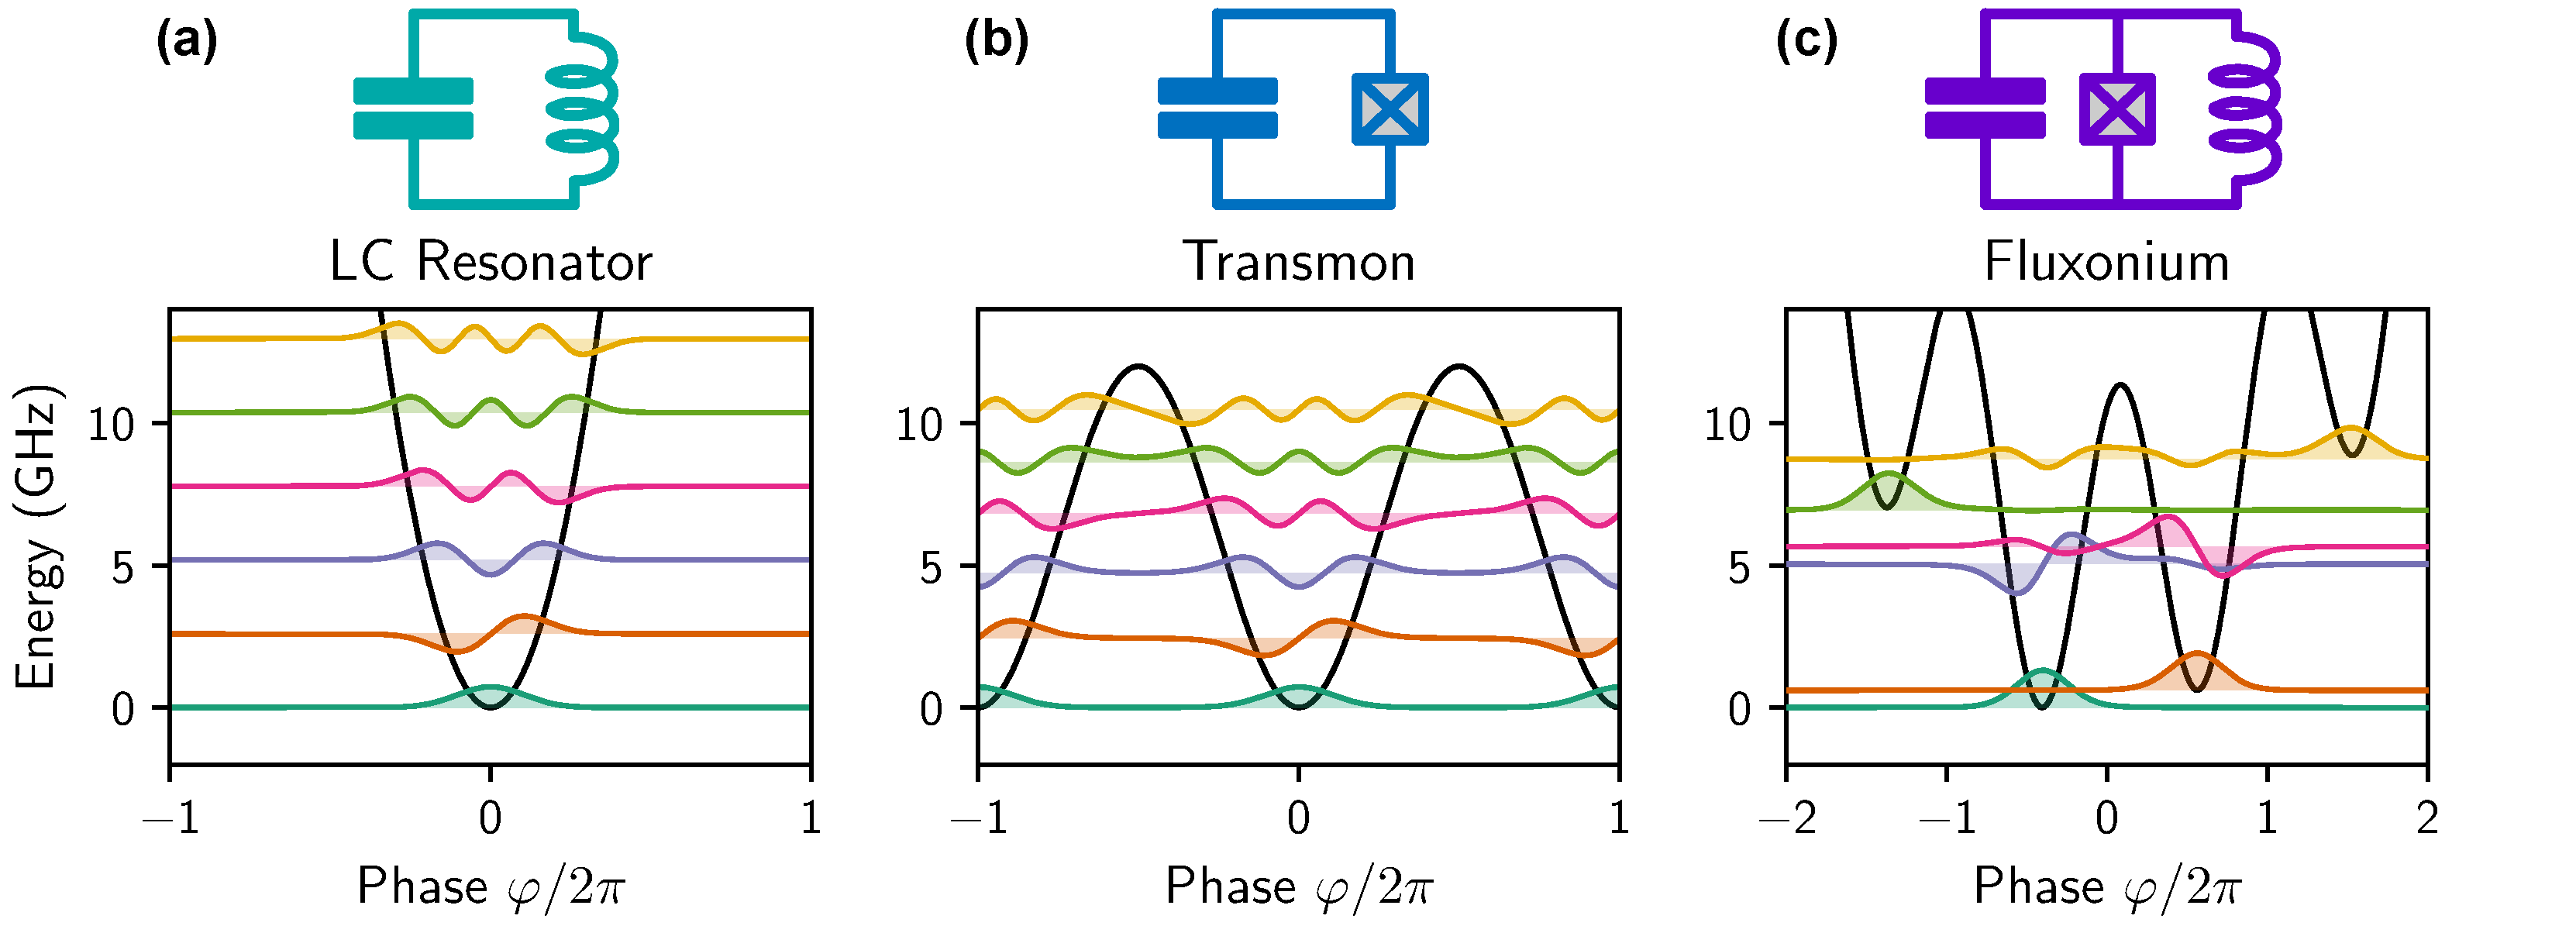
\includegraphics[width=\linewidth]{Figures/3/Circuit_QED_Overview.pdf}
    \caption[Overview of Circuit QED, showing the circuit diagrams, potentials, and wavefunctions for the LC Resonator, the transmon qubit, and the fluxonium qubit.]{\textbf{The LC resonator, transmon, and fluxonium.} We show the circuit diagrams, potentials (black), and wavefunctions (colored) for each of the three common superconducting circuits. \textbf{(a)} LC resonator parameters are $E_L/h = 6$ GHz and $E_C/h = 0.14$ GHz. \textbf{(b)} Transmon qubit parameters are $E_J/h = 6$ GHz and $E_C/h = 0.14$ GHz. \textbf{(c)} Fluxonium qubit parameters are $E_J/h = 6$ GHz,  $E_L/h = 0.2$ GHz, $E_C/h = 0.14$ GHz, \& $\Phi_{\rm ext} = 0.42\Phi_0$.}
    \label{fig:3_Circuit_QED_Overview}
\end{figure}
\clearpage

\section{The LC Resonator}

As its name suggests, an LC circuit consists of a capacitor with capacitance $C$ and inductor with inductance $L$ in parallel. Following Ref. \cite{krantz2019quantum}, we can write a classical Hamiltonian for the LC circuit in terms of the voltage $V(t)$ across the capacitor and the current $I(t)$ flowing through the inductor. These two circuit elements have energies $\frac{1}{2}CV^2$ and $\frac{1}{2}LI^2$ respectively, and thus
\begin{equation}
    H = \frac{1}{2}CV^2 + \frac{1}{2}LI^2
\end{equation}
This Hamiltonian is reminiscent of that of the harmonic oscillator, which we studied in detail in Ch. \ref{ch:2_QEC}. Indeed, if we look at the classical response of this circuit, we find that it behaves like a resonator with resonance frequency $\omega = 1/\sqrt{LC}$. The classical Hamiltonian above can equivalently be written in terms of the charge $Q(t) = CV(t)$ and the flux through the inductive loop $\Phi(t) = LI(t)$. Following \cite{devoret1995quantum}, it will be most convenient to work in terms of these variables so that:
\begin{equation}
    H = \frac{Q^2}{2C} + \frac{\Phi^2}{2L}
\end{equation}
Under this canonical representation, we can think of the flux variable $\Phi$ as a position-like variable of a harmonic oscillator, with the charge variable $Q$ representing the generalized conjugate momentum. We now perform \textit{circuit quantization}, promoting these variables to quantum mechanical operators: $\Phi \to \hat{\Phi}$ and $Q \to \hat{Q}$. We can therefore write the \textit{quantum} Hamiltonian as
\begin{equation}
    \hat{H} = \frac{\hat{Q}^2}{2C} + \frac{\hat{\Phi}^2}{2L} = 4E_C \hat{n}^2 + \frac{1}{2}E_L \hat{\varphi}^2
\end{equation}
where in the second step we define the reduced charge operator $\hat{n} = \hat{Q}/2e$ and reduced phase operator $\hat{\varphi} = 2\pi \hat{\Phi}/\Phi_0$ where $e$ is the electron charge, $\Phi_0 = h/2e$ is the magnetic flux quantum, and we have also defined the charging and inductive energies $E_C = e^2/2C$ and $E_L = (\Phi_0/2\pi)^2/L$ respectively. The operators $\hat{\Phi}$ and $\hat{\Phi}$ are conjugate variables satisfying the canonical commutation relation $[\hat{\Phi}, \hat{Q}] = i\h$, and we can easily check that $[\hat{\varphi}, \hat{n}] = i\h$ as well. Continuing with the analogy to mechanical oscillators, we refer to the inductive term as the potential energy, and the charge term as a kinetic energy. As it will be useful later, we can also define the characteristic \textit{impedance} $Z = \sqrt{L/C}$

As a final step, we can introduce \textit{mode} operators $\hat{a}, \hat{a}^\dagger$ just as we did in Ch. \ref{ch:2_QEC}. We define the transformation
\begin{equation}
    \hat{\varphi} = \varphi_{\rm zpf}(\hat{a} + \hat{a}^\dagger), \quad \hat{n} = in_{\rm zpf}(\hat{a}^\dagger - \hat{a})
\end{equation}
in terms of the zero-point fluctuations $\varphi_{\rm zpf} = (2E_C/E_L)^{1/4}$ and $n_{\rm zpf} =  [E_L/(32E_C)]^{1/4}$ so as to rewrite the Hamiltonian as
\begin{equation}
    \hat{H} = \h\omega\bigg(\hat{a}^\dagger\hat{a} + \frac{1}{2}\bigg)
    \label{eq:3_LC_QHO}
\end{equation}
with $\h\omega = \sqrt{8 E_LE_C}$. We can now use the intuition we developed in Ch. \ref{ch:2_QEC}, and in particular conclude that the LC resonator has Fock states $\ket{n}$ with energy levels $E_n = \h\omega(n+1/2)$. As before, we will typically drop the constant term $\h\omega/2$ in theory derivations. We plot the phase wavefunctions $\psi_n(\varphi)$ associated with these states in Fig. \ref{fig:3_Circuit_QED_Overview} using the parameters $E_C/h = 0.14$ GHz and $E_L/h = 6$ GHz. 

To give some context, superconducting LC circuits are typically operated at microwave frequencies of 1-10 GHz, and are cooled down to ambient temperatures of $T \simeq 20$ mK via a dilution refrigerator. In this limit, we have $k_BT \ll \h\omega$ and thus do not expect significant thermal population of the resonator states. 

To control the LC oscillator, we typically use an external \textit{classical} voltage bias $V_b(t)$ that couples to the circuit via its charge operator; physically, this is realized by some drive line or port that is capacitively coupled. In this case, the driven Hamiltonian can be written as follows:
\begin{equation}
    \hat{H}(t) = \frac{\hat{Q}^2}{2C} + \frac{\hat{\Phi}^2}{2L} + \hat{Q}V_b(t) = \h\omega\hat{a}^\dagger\hat{a} + i\Omega(t) (\hat{a}^\dagger - \hat{a})
\end{equation}
where $\Omega(t) = 2eV_b(t)n_{\rm zpf}$ is typically assumed to have the form $\Omega(t) = \Omega_0\cos(\omega_d t)$ in terms of a drive frequency $\omega_d$ and amplitude $\Omega_0$. As we saw in Sec. \ref{sec:2_control_nonlinearity_drive}, such a classical drive can only produce coherent states in the oscillator. Put equivalently, the resonator energies $E_n$ are all equidistant (with spacing $\h\omega)$, and thus there is no uniquely addressable transition frequency that we can use to create a two-level system (i.e., qubit) from. Therefore, if we want to create a superconducting qubit, we need to introduce some form of \textit{nonlinearity} to the system. 


\section{The Transmon Qubit}

\subsection{Nonlinearity and the Josephson Junction}

We have seen that nonlinearity is a necessary feature for building superconducting qubits. In circuit QED, there is only one circuit element that is both nonlinear and non-dissipative at arbitrarily low temperatures: the Josephson junction, also known as a superconducting tunnel junction \cite{devoret2004superconducting}. Josephson junctions are comprised of two pieces of superconducting metal separated by an insulating layer that is thin enough to allow discrete charges of the superconductor (i.e., Cooper pairs) to tunnel through the barrier. Typically,  junctions are fabricated using aluminium as the superconductor and aluminium oxide as the insulating barrier. The theory behind the Josephson junction is intimately tied to the Bardeen–Cooper–Schrieffer (BCS) theory of superconductivity. While we will not delve into these details here, I recommend the classic text \textit{Introduction to Superconductivity} by Tinkham for a discussion of this \cite{tinkham2004introduction}. Practically, the Josephson junction as a circuit element can be thought of as a nonlinear inductor. It satisfies a current-phase relationship defined by the Josephson equations:
\begin{equation}
    I = I_c \sin(\varphi), \, V = \frac{\h}{2e}\frac{d\varphi}{dt}
    \label{eq:3_josephson_eqs}
\end{equation}
Here $I_c$ is the so-called \textit{critical current} of the junction (i.e., the maximum supercurrent it can support) and $\varphi$ is a variable known as the gauge-invariant phase difference \cite{devoret2021does}, which when quantized can be associated with the reduced phase operator $\hat{\varphi}$. Using Eq. \eqref{eq:3_josephson_eqs}, we find that the inductive potential energy $U(\varphi)$ associated with the Josephson junction is $U(\varphi) = -E_J\cos(\varphi)$ with the so-called \textit{Josephson energy} $E_J$ defined as $E_J = I_c\Phi_0/2\pi$. There is also a finite capacitance $C_J$ associated with a junction, which will give rise to a kinetic energy term $4E_C\hat{n}^2$ in the quantum Hamiltonian\footnote{This is also the Hamiltonian of an older qubit known as the Cooper-Pair Box (CPB) which consisted of just a junction and an external voltage bias. The bias gives rise to an offset voltage or \textit{gate charge} $n_g$ which enters the Hamiltonian via $\hat{H} = 4E_C(\hat{n}-n_g)^2 - E_J\cos(\hat{\varphi})$. However, in the so-called transmon regime that we will discuss in the next section, the gate charge $n_g$ can safely be ignored for the static circuit. } of the junction, which is simply given as the total energy $\hat{H} = 4E_C\hat{n}^2 - E_J\cos(\hat{\varphi})$, with $E_C = e^2/2C_J$. 

\subsection{Hamiltonian of the Transmon}

The \textit{transmon} qubit is formed by placing a Josephson junction in parallel with a large shunt capacitance $C_s$. This capacitance can be added to the intinsic capacitance of the junction $C_J$ to get a total $C_\Sigma = C_J + C_s$. The transmon circuit is shown in Fig. \ref{fig:3_Circuit_QED_Overview} and gives rise to the Hamiltonian
\begin{equation}
    \hat{H} = 4E_C\hat{n}^2 - E_J\cos(\hat{\varphi})
    \label{eq:3_transmon_H}
\end{equation}
with $E_C = e^2/2C_\Sigma$. Since the shunt capacitance is large, the transmon is typically operated in the regime $E_J \gg E_C$. We plot the cosine potential and phase-basis wavefunctions for a transmon in Fig. \ref{fig:3_Circuit_QED_Overview}, using the parameters $E_J/h = 6$ GHz and $E_C/h = 0.14$ GHz. 

In the transmon regime, the phase operator $\hat{\varphi}$ satisfies $\Delta\hat{\varphi} = \sqrt{\ev{\hat{\varphi}^2} - \ev{\hat{\varphi}}^2} \ll 1$, i.e., the phase fluctuations are small. Specifically, if we ignore the periodicity of the potential, we find that the wavefunctions in the region $\varphi \in [-\pi, \pi]$ are well-localized near the bottom of the potential well around $\varphi = 0$, at least for the low-lying energy states. In this case, we can Taylor expand the potential energy term as a power series in $\hat{\varphi}$. More rigorously, it is possible to write  
\begin{equation}
    \hat{H} = 4E_C\hat{n} + \frac{1}{2}E_J \hat{\varphi}^2 - E_J\bigg[\cos(\hat{\varphi}) + \frac{1}{2}E_J \hat{\varphi}^2\bigg]
\end{equation}
The first two terms can be expressed in terms of oscillator-like mode operators $\hat{q}, \hat{q}^\dagger$ defined as $\hat{\varphi} = \varphi_{\rm zpf}(\hat{q} + \hat{q}^\dagger)$ and $\hat{n} = in_{\rm zpf}(\hat{q}^\dagger - \hat{q})$ with $\varphi_{\rm zpf} = (2E_C/E_J)^{1/4}$ and $n_{\rm zpf} =  [E_J/(32E_C)]^{1/4}$. In the transmon regime, $\varphi_{\rm zpf} \ll 1$ and so we can expand the remaining nonlinear term. To leading order,
\begin{equation}
    \hat{H} \approx 4E_C\hat{n}^2 + \frac{1}{2}E_J \hat{\varphi}^2 - \frac{E_J}{24}\hat{\varphi}^4 = \h\omega_q \hat{q}^\dagger \hat{q} - \frac{E_C}{12}(\hat{q} + \hat{q}^\dagger)^4
    \label{eq:transmon_duffing_H}
\end{equation}
where $\h\omega_q = \sqrt{8 E_C E_J}$. When written this way, it is immediately evident that the transmon is essentially a nonlinear oscillator. Using perturbation theory, we find that the energies are approximately \cite{bishop2010circuit}:
\begin{equation}
    E_m \simeq m\h\omega_q - \frac{E_C}{12}\big[6m^2 + 6m\big]
\end{equation}
which, as desired for a qubit, are nonlinear in $m$. To get to this, we can expand the quartic nonlinearity and, after normal ordering, keep only the number-conserving terms $\hat{q}^\dagger{}^n\hat{q}^n$, which is tantamount to performing a rotating-wave approximation. Doing so, we get the simplified Hamiltonian
\begin{equation}
    \hat{H} = \h[\omega_q + \alpha]\hat{q}^\dagger \hat{q} + \frac{\h\alpha}{2}\hat{q}^\dagger{}^2\hat{q}^2
\end{equation}
where we have defined the \textit{anharmonicity} as $\h\alpha = -E_C$, and we refer to $\omega_{\rm ge} = \omega_q + \alpha$ as the qubit transition frequency. Since the $\ket{g}\to\ket{e}$ and $\ket{e}\to\ket{f}$ transitions are now detuned from each other by $\alpha = \omega_{ef}-\omega_{ge}$, we can treat the lowest two levels $\ket{g}$ and $\ket{e}$ as a two-level qubit, for which
\begin{equation}
    \hat{H} \approx \frac{\h\omega_{\rm ge}}{2}\sigmaz
\end{equation}
Here, we made a two-level approximation $\hat{q} \to \sigmam$, $\hat{q}^\dagger \to \sigmap$ and so $\hat{q}^\dagger \hat{q} \to (1 - \sigmaz)/2$ and we drop the minus sign by convention. Finally, to give perspective, typical transmons have frequencies $\omega_{\rm ge}$ in the range of 4-6 GHz, and anharmonicities $|\alpha|$ around 100-400 MHz. 

\noindent Note: here, we explicitly kept the $\h$ factor in the Hamiltonian throughout the calculation. However, in subsequent derivations, we will often set $\h \to 1$ for convenience and brevity, i.e., mixing frequency and energy units. We leave it to the reader to infer when to insert the appropriate factors of $\h$ into relevant expressions. Thus, going forward, we will often write $\hat{H} = \omega \hat{a}^\dagger\hat{a}$ for a resonator Hamiltonian, or $\hat{H} = \omega_{\rm ge}\sigmaz/2$ for a qubit Hamiltonian. 

\subsection{Coupling a Transmon and a Resonator}

The basis of circuit QED involves coupling superconducting qubits and resonators to form a spin-oscillator model. Thus, let us briefly touch on how we couple a transmon qubit to an LC resonator. We typically use a capacitive coupling model with an interaction of the form $\hat{H}_{\rm int} = J_{aq} \hat{n}_a \hat{n}_q$ with coupling strength $J_{aq}$ between the charge operators of the oscillator and qubit respectively. The total Hamiltonian for the coupled system is given by
\begin{equation}
    \hat{H} = \hat{H}_a + \hat{H}_q + \hat{H}_{\rm int} = \omega_a \hat{a}^\dagger\hat{a} + \Big[4E_C\hat{n}^2 - E_J\cos(\hat{\varphi})\Big] + \hat{H}_{\rm int}
    \label{eq:3_transmon_resonator_full}
\end{equation}
Expressing the transmon in terms of its mode operators and defining $g = -J_{aq}n_{{\rm zpf},a}n_{{\rm zpf},q}$, we have 
\begin{equation}
    \hat{H} = \omega_a \hat{a}^\dagger\hat{a} + \omega_{\rm ge}\hat{q}^\dagger \hat{q} + \frac{\alpha}{2}\hat{q}^\dagger{}^2\hat{q}^2 + g(\hat{a}-\hat{a}^\dagger)(\hat{q}-\hat{q}^\dagger)
    \label{eq:3_transmon_resonator_linear_coupling}
\end{equation}
with a bilinear coupling in $\hat{a}$ and $\hat{q}$. At this point, we can truncate to a two-level qubit and perform a rotating-wave approximation (RWA) on the coupling term, which is standard in the literature \cite{blais2021circuit}. Doing so will give us a Jaynes-Cummings type Hamiltonian as we saw in Sec. \ref{sec:2_control_nonlinearity_drive}:
\begin{equation}
    \hat{H} = \omega_a \hat{a}^\dagger\hat{a} + \frac{\omega_{\rm ge}}{2}\sigmaz + \big[\hat{a}^\dagger\sigmam + \hat{a}\sigmap\big]
    \label{eq:3_JC_Hamiltonian_transmon}
\end{equation}
As we did there, we can further transform this Hamiltonian to a dispersive coupling model in the limit $g \ll |\omega_a - \omega_{\rm ge}|$. For a truly two-level system starting from Eq. \eqref{eq:3_JC_Hamiltonian_transmon}, this gives the Hamiltonian
\begin{equation}
    \hat{H}_{\rm disp} = \omega_a' \hat{a}^\dagger\hat{a} + \frac{\omega_{\rm ge}'}{2}\sigmaz + \frac{\chi}{2}\hat{a}^\dagger\hat{a}\sigmaz
    \label{eq:3_dispersive_model_transmon_TLS}
\end{equation}
with the definitions $\chi = 2g^2/\Delta$, $\omega_a' = \omega_a$, and $\omega_{\rm ge}' = \omega_{\rm ge} + g^2/\Delta$ in terms of $\Delta = \omega_{\rm ge} - \omega_a$. As we previously saw, this dispersive Hamiltonian forms the basis of most of modern circuit QED and also gives a blueprint for qubit readout, since we can determine the qubit state by measuring the effective frequency $\omega_a' + \chi \hat{a}^\dagger\hat{a}\ev{\sigmaz}/2$ of the resonator \cite{blais2004cavity}. 

For realistic transmons, it turns out to be not quite correct to truncate to a two-level qubit before making the dispersive approximation. If we instead make the dispersive approximation at the level of Eq. \eqref{eq:3_transmon_resonator_linear_coupling} and \textit{then} truncate, we get a final Hamiltonian with the same form as Eq. \eqref{eq:3_dispersive_model_transmon_TLS} but with redefined $\omega_a' = \omega_a - g^2/(\Delta - E_C/\h)$, $\omega_{\rm ge}' = \omega_{\rm ge} + g^2/\Delta$, and $\chi = - (g^2E_C/\h) / [\Delta(\Delta - E_C/\h)]$. 

\noindent\textbf{Black-Box Quantization.} There is another way to treat a coupled transmon and resonator known as black-box quantization (BBQ) that makes use of the oscillator-like character of the transmon \cite{nigg2012black}. Starting from the full model in Eq. \eqref{eq:3_transmon_resonator_full}, we can write the Hamiltonian as:
\begin{equation}
    \hat{H} = \omega_a \hat{a}^\dagger\hat{a} + \omega_q \hat{q}^\dagger\hat{q} + g(\hat{a}-\hat{a}^\dagger)(\hat{q}-\hat{q}^\dagger) - E_J\bigg[\cos(\hat{\varphi}) + \frac{1}{2}E_J \hat{\varphi}^2\bigg]
\end{equation}
The first three terms describe two linearly coupled oscillators which can be diagonalized exactly via a Bogolioubov transformation to get two normal modes $\hat{a}'$ (oscillator-like) and $\hat{q}'$ (qubit-like) with frequencies $\omega_a'$ and $\omega_q'$. The phase of the transmon $\hat{\varphi} = \varphi_{\rm zpf}(\hat{q} + \hat{q}^\dagger)$ can then be expressed as a superposition of the new modes $\hat{\varphi} = \varphi_a(\hat{a}' + \hat{a}'{}^\dagger) + \varphi_q(\hat{q}' + \hat{q}'{}^\dagger)$ with \textit{participation ratios} $\varphi_a$, $\varphi_q$ that can be extracted from the diagonalization. At this point, we can now truncate the nonlinear potential term of the transmon and keep just the quartic term $-E_J\hat{\varphi}^4/24$. For brevity, but at the risk of confusion, I now drop the $'$ superscripts and write
\begin{equation}
    \hat{H} = \omega_a \hat{a}^\dagger\hat{a} + \omega_q \hat{q}^\dagger\hat{q} - \frac{E_J}{24}\big[\varphi_{a}(\hat{a} + \hat{a}^\dagger) + \varphi_{q}(\hat{q} + \hat{q}^\dagger)\big]^4
\end{equation}
\textit{in the normal mode basis} (this is important to keep in mind; we really mean $\hat{a}'$ and $\hat{q}'$ above). From here, we can expand the quartic term to get various monomials. Again invoking the RWA, we keep only the number-conserving terms in the expansion. This gives an effective Hamiltonian:
\begin{equation}
    \hat{H} = \omega_a \hat{a}^\dagger\hat{a} + \omega_q \hat{q}^\dagger\hat{q} + \frac{\chi_{aq}}{2}\hat{a}^\dagger\hat{a}\hat{q}^\dagger\hat{q}  + \frac{K_a}{2}\hat{a}^\dagger{}^2\hat{a}^2 + \frac{K_q}{2}\hat{q}^\dagger{}^2\hat{q}^2
    \label{eq:3_transmon_resonator_BBQ}
\end{equation}
where we now have a dispersive shift $\chi_{aq} \triangleq -E_J\varphi_a^2 \varphi_q^2/2$ and so-called \textit{Kerr} nonlinearities $K_q \triangleq -E_J\varphi_q^4/4$ and $K_a \triangleq -E_J\varphi_a^4/4$ for the qubit and oscillator, with the former just being the qubit's anharmonicity. From these expressions, we get the interesting and often useful geometric mean relation $\chi_{aq}^2 = 4K_aK_q$ for relating the Kerr nonlinearities to the dispersive shift. The ``BBQ'' Hamiltonian above in Eq. \eqref{eq:3_transmon_resonator_BBQ} is similar to that in Eq. \eqref{eq:3_dispersive_model_transmon_TLS} in that it has a dispersive coupling, but differs in that the oscillator now inherits some nonlinearity as well. This can be particularly harmful when we are trying to use oscillators for bosonic QEC (e.g. with a GKP code), since bosonic codes typically assume a linear oscillator mode. 

We will return to black-box quantization with the transmon in Ch. \ref{ch:5_2DGKP}, where we develop a novel theoretical proposal for GKP error correction using a microwave-activated coupler element and a transmon control qubit. Moreover, we will show how the idea behind BBQ (i.e., working in the basis of linearized modes) can be extended to coupled driven quantum systems with fluxonium too\footnote{In the literature, coupled systems featuring a fluxonium qubit have not typically been studied in this way before. More details about this approach can also be found in the upcoming SM thesis of Shantanu Jha.}. 

% \vfill
% \begin{greybox}
%     \textbf{Generalization of black-box quantization:} We use the black-box quantization (BBQ) approach extensively in our research 
% \end{greybox}
% \todo{} Maybe mention how we have generalized BBQ?

\clearpage
\section{The Fluxonium Qubit}

We are now ready to discuss the main qubit of interest for this thesis: the fluxonium \cite{manucharyan2009fluxonium}. A fluxonium consists of a linear inductor, a capacitor, and a Josephson junction in parallel, with energies $E_L$, $E_C$, and $E_J$ respectively. A corresponding circuit diagram for this qubit is shown in Fig. \eqref{fig:3_Circuit_QED_Overview}. While it may be tempting to simply add together the various energy terms that we have seen previously, there is one additional piece of theoretical background required, known as \textit{flux quantization}. 

Fluxonium is a type of generalized \textit{flux qubit}, and thus it is possible to thread an external magnetic flux $\Phi_{\rm ext}$ through the loop between the junction and the inductor. If we define the branch variables $\Phi_J$ and $\Phi_L$ for these two elements respectively, then the flux quantization condition can be expressed \cite{orlando1991foundations}:
\begin{equation}
    \Phi_J - \Phi_L = \Phi_{\rm ext}
\end{equation}
This is a holonomic constraint on the phase variables; there is thus only one effective phase degree of freedom in the circuit. Working in terms of the reduced variables $\varphi_k = 2\pi \Phi_k/\Phi_0$, we can choose to allocate\footnote{Note that for \textit{time-dependent} external fluxes $\varphi_{\rm ext} = \varphi_{\rm ext}(t)$, the choice of allocation becomes more subtle and it turns out we should instead group the external flux with the inductor $\varphi_L = \varphi - \varphi_{\rm ext}$. After performing circuit quantization, the fluxonium Hamiltonian then reads $\hat{H} = 4E_C \hat{n}^2 + \frac{1}{2}E_L[\hat{\varphi} - \varphi_{\rm ext}]^2 - E_J\cos(\hat{\varphi})$ \cite{you2019circuit}.} the external flux via $\varphi_J = \varphi + \varphi_{\rm ext}$ and $\varphi_L = \varphi$. The inductive energy of the inductor is then $\frac{1}{2}E_L\varphi^2$, while the Josephson energy is $-E_J\cos(\varphi + \varphi_{\rm ext})$. We therefore finally get
\begin{equation}
    \hat{H} = 4E_C \hat{n}^2 + \frac{1}{2}E_L\hat{\varphi}^2 - E_J\cos(\hat{\varphi} + \varphi_{\rm ext})
    \label{eq:3_fluxonium_H}
\end{equation}
for the fluxonium Hamiltonian after circuit quantization. In practice, the inductive energy is $E_L \sim 0.5$ GHz, corresponding to a large inductance $L \sim 325$ nH \cite{nguyen2022blueprint}. There are various approaches to realize such a \textit{superinductance}, such as using granular aluminum \cite{maleeva2018circuit, grunhaupt2019granular, kamenov2020granular, rieger2023granular} or geometric inductances \cite{peruzzo2020surpassing, peruzzo2021geometric}, but by far the most common strategy is to use an array of Josephson junctions \cite{manucharyan2009fluxonium, masluk2012microwave}, as we show in Fig. \ref{fig:3_Superinductance}. A nice pedagogical derivation of how a chain of $N$ Josephson junctions behaves like a linear inductor in the limit of large $N$ can be found in the excellent PhD thesis of EQuS alum Leon Ding \cite{ding2023thesis}. 

\begin{figure}
    \centering
    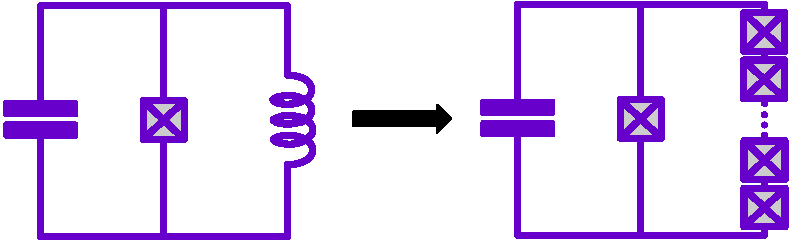
\includegraphics[width=0.7\linewidth]{Figures/3/Superinductance.pdf}
    \caption[Superinductance in a fluxonium qubit comprised of an array of Josephson junctions.]{The superinductance in a fluxonium is typically implemented via an array of $N$ Josephson junctions, which behave approximately like a linear inductor for large $N$.}
    \label{fig:3_Superinductance}
\end{figure}

As a final remark on the Hamiltonian, we note that the inductive and charging terms of Eq. \eqref{eq:3_fluxonium_H} can be diagonalized using the $E_L$-$E_C$ Fock basis, as done for the LC circuit. This allows us to write
\begin{equation}
    \hat{H} = \h\omega_q\hat{q}^\dagger\hat{q} - E_J\cos(\hat{\varphi} + \varphi_{\rm ext})
\end{equation}
for the \textit{full} Hamiltonian, with $\h\omega_q = \sqrt{8 E_LE_C}$ and $\hat{\varphi} = (2E_C/E_L)^{1/4}[\hat{a} + \hat{a}^\dagger]$ as in Eq. \eqref{eq:3_LC_QHO}. Using this basis, it is possible to numerically diagonalize the full fluxonium Hamiltonian. We plot an example of this with the phase-basis wavefunctions in Fig. \ref{fig:3_Circuit_QED_Overview}. As before, we note that we will set $\h \to 1$ for brevity in the upcoming theory derivations. 

The regime we are interested in for the fluxonium is the so-called heavy regime in which $E_J \gg E_C$. When $\Phi_{\rm ext} = 0.5\Phi_0$, the potential energy has a double-well structure, with the lowest energy states $\ket{g}$ and $\ket{e}$ given by symmetric and antisymmetric combinations of the two wells' localized wavefunctions, and the qubit frequency $\omega_{\rm ge}$ becomes small; the heaviness of a fluxonium can be characterized by the splitting $\omega_{\rm ge}$ at this half-flux point. Typical heavy fluxonium devices have qubit frequencies of about 10-300 MHz, with lower $\omega_{\rm ge}$ translating to ``heavier'' \cite{earnest2018realization, zhang2021universal, ding2023FTF}. Meanwhile, if we move slightly off this half-flux point, the ground and excited states will have a larger energy splitting and be strongly localized to their respective wells, as is shown in Fig. \ref{fig:3_Circuit_QED_Overview}. When operated as a low-frequency qubit, the fluxonium has $\omega_{\rm ge} \ll \alpha$ (the anharmonicity), which truly enables us to think of it as a two-level system. Also, the charge matrix element vanishes $\mel{g}{\hat{n}}{e} \to 0$. This in turn has led to heavy fluxonium qubits reporting $T_1$ lifetimes (between states $\ket{g}$ and $\ket{e}$) in excess of 1 ms at the half-flux sweet spot, and typically even larger away from it \cite{earnest2018realization, zhang2021universal, ding2023FTF, nguyen2019high, somoroff2023millisecond}. It is for this reason that we are interested in the fluxonium as a bit-flip protected control qubit. 

\subsection{Circuit QED with the Fluxonium\label{sec:3_Circuit_QED_with_Fluxonium}}

Just as we did for the transmon, let's now briefly examine how to couple a fluxonium to a harmonic oscillator. The basic model we follow is that of Ref. \cite{zhu2013cQEDfluxonium}, which starts from the Hamiltonian
\begin{equation}
    \hat{H} = \sum_k \omega_k \op{k}{k} + \omega_a \hat{a}^\dagger\hat{a} + g\hat{n}(\hat{a} + \hat{a}^\dagger)
    \label{eq:3_fluxonium_cQED}
\end{equation}
in terms of the bare fluxonium eigenstates $\ket{k}$ and coupling strength $g$. When we deal with this Hamiltonian in practice, we will typically just numerically diagonalize it and compute the hybridized energy levels $E_{k, n}$ associated with a qubit state $k$ and resonator state $n$; to be more precise, we diagonalize the coupled system to get the unlabelled eigenenergies $\lambda_i$ and eigenstates $\ket{v_i}$ and then perform \textit{quantum number assignment} to label each state $\ket{v_i}$ in terms of the uncoupled basis state $\ket{k}\otimes\ket{n}$ that it is closest to (i.e., largest overlap). In this way, we can get the \textit{labelled} energies $E_{k, n}$ and eigenstates $\ket{k, n}$ for the hybridized system. Note that implicit in this approach is the assumption that $g$ is a small parameter, i.e., we can treat the coupling as a perturbation and assign meaningful quantum numbers. In this limit, Eq. \eqref{eq:3_fluxonium_cQED} admits a dispersive approximation given (after normal ordering) by \cite{zhu2013cQEDfluxonium}:
\begin{equation}
    \hat{H}_{\rm disp} = \omega_a \hat{a}^\dagger\hat{a} + \sum_k (\omega_k + \delta_k' + \delta_k'') \op{k}{k} + \sum_k \bigg[\Big(\chi_k' + \chi_k'' + \frac{K_k''}{2}\Big)\hat{a}^\dagger\hat{a} + \frac{K_k''}{2}\hat{a}^\dagger{}^2\hat{a}^2\bigg] \op{k}{k}
    \label{eq:3_fluxonium_cQED_pert_theory}
\end{equation}
This Hamiltonian is computed using 2nd- and 4th-order perturbation theory (1st and 3rd order are zero). We get qubit Lamb shifts $\delta'$ and $\delta''$ from 2nd and 4th order terms respectively; likewise, we get dispersive shifts $\chi_k'$ and $\chi_k''$ of qubit state $\ket{k}$ to the oscillator, as well as Kerr nonlinearities $K_k''$ (which come only from the 4th order corrections). The full perturbation theory expressions for these various energy terms are rather unweildy but can be found in Ref. \cite{zhu2013cQEDfluxonium}. For our purposes, we consider a simpler rewriting of Eq. \eqref{eq:3_fluxonium_cQED_pert_theory}, given by
\begin{equation}
    \hat{H}_{\rm disp} = \omega_a \hat{a}^\dagger\hat{a} + \sum_k \tilde{\omega}_k \op{k}{k} + \sum_k \bigg[\chi_k\hat{a}^\dagger\hat{a} + \frac{K_k}{2}\hat{a}^\dagger{}^2\hat{a}^2\bigg] \op{k}{k}
\end{equation}
in terms of effective qubit frequencies $\tilde{\omega}_k$,  dispersive shifts $\chi_k$ and Kerrs $K_k$. We can connect these to the results we get from numerical diagonalization, expressing them in terms of the numerically obtained system energies $E_{k, n}$. The Kerr nonlinearities $K_k$ are simply given by the resonator anharmonicity when the qubit is in state $\ket{k}$, which we can compute as follows:
\begin{equation}
    K_k = [E_{k, 2} - E_{k, 1}] - [E_{k, 1} - E_{k, 0}] = E_{k, 2} + E_{k, 0} - 2E_{k, 1}
\end{equation}
Meanwhile, we get an effective  resonator frequency $\omega_a^{\ket{k}}$ that depends on the qubit state. It is given by
\begin{equation}
    \omega_a^{\ket{k}} = \omega_a + \chi_k = E_{k, 1} - E_{k, 0}
\end{equation}
Finally, the qubit transitions $\tilde{\omega}_k$ are the `renormalized' frequencies, and computed via $E_{k, 0}$. At this point, after numerically diagonalizing using the full fluxonium-oscillator model, we can safely truncate the fluxonium to a two-level system for $\Phi_{\rm ext} \approx 0.5\Phi_0$ (the external flux tunes the various energies above). In this case, we focus on only the two qubit state $\ket{g}$ and $\ket{e}$ in the sums above. Furthermore, it will be useful to define an effective dispersive shift
\begin{equation}
    \chi \equiv \omega_s^{|e\rangle} - \omega_s^{|g\rangle} = [E_{1,1} - E_{1, 0}] - [E_{0, 1} - E_{0, 0}]  = \chi_e - \chi_g
\end{equation}
as the difference in the resonator frequency when the qubit is in $\ket{g}$ vs. $\ket{e}$. Putting this all together, we can therefore write down an effective dispersive model for the system: 
\begin{equation}
    \hat{H} = \omega_a \hat{a}^\dagger\hat{a} + \frac{\tilde{\omega}_{\rm ge}(\varphi_{\rm ext})}{2} \sigmaz + \frac{\chi(\varphi_{\rm ext})}{2}\hat{a}^\dagger\hat{a}\sigmaz  + \frac{K_g(\varphi_{\rm ext})}{2}\hat{a}^\dagger{}^2\hat{a}^2\op{g}{g} + \frac{K_e(\varphi_{\rm ext})}{2}\hat{a}^\dagger{}^2\hat{a}^2\op{e}{e}
\label{eq:3_fluxonium_cQED_TLS}
\end{equation}
This closely resembles the other dispersive qubit-oscillator Hamiltonians that we studied in this chapter, except now the qubit frequency $\tilde{\omega}_{ge} = \tilde{\omega}_{e} - \tilde{\omega}_{g}$, dispersive shift $\chi$, and Kerr nonlinearities $K_g$, $K_e$ all tune with the external flux $\varphi_{\rm ext}$, a features that will be incredibly useful when designing a bosonic QEC experiment, as we will discuss in Ch. \ref{ch:4_3DGKP}. Lastly, one can also rewrite Eq. \eqref{eq:3_fluxonium_cQED_TLS} in terms of an \textit{average} Kerr $K = [K_g + K_e]/2$ and what we call a \textit{differential} Kerr $dK = [K_g + K_e]/2$, to better match previous expressions. In this case:
\begin{equation}
    \hat{H} = \omega_a \hat{a}^\dagger\hat{a} + \frac{\tilde{\omega}_{\rm ge}(\varphi_{\rm ext})}{2} \sigmaz + \frac{\chi(\varphi_{\rm ext})}{2}\hat{a}^\dagger\hat{a}\sigmaz  + \frac{K(\varphi_{\rm ext})}{2}\hat{a}^\dagger{}^2\hat{a}^2 + \frac{dK(\varphi_{\rm ext})}{2}\hat{a}^\dagger{}^2\hat{a}^2\sigmaz
\end{equation}
We will use this Hamiltonian going forward when discussing our experiments. 
\clearpage
% % ------------------------------------------------

% %%%%% Chapter 4: 3D GKP Project %%%%%%
\chapter{Fluxonium in a 3D Cavity: Experiments\label{ch:4_3DGKP}}

\section{Experimental Design and Theory \label{sec:4_3D_Experiment_Design_Theory}}

In this section, we 

$$
\hat{H} = \hat{H}_q + \hat{H}_a + \hat{H}_{\rm int} = \Big[4E_C \hat{n}^2 + \frac{1}{2}\hat{\varphi}^2 - E_J\cos(\hat{\varphi}-2\pi\phi_{\rm ext})\Big] + \omega_s \hat{a}^\dagger \hat{a} + J \hat{n}\hat{n}_a
$$

Here the term in parentheses is the qubit Hamiltonian defined in terms of the fluxonium $E_C$, $E_J$, and $E_L$ parameters, as well as the external flux $\phi_{\rm ext} = \Phi_{\rm ext}/\Phi_0$. The storage oscillator mode is defined in terms of its annihilation operator $\hat{a}$, its frequency $\omega_s$ and its zpf $\varphi_{a, \rm zpf}$, which defines:

\begin{align*}
\hat{\varphi}_a &= \varphi_{a, \rm zpf} (\hat{a}+\hat{a}^\dagger) \\
\hat{n}_a &= \frac{i}{2\varphi_{a, \rm zpf}} (\hat{a}^\dagger - \hat{a})
\end{align*}

Finally, the coupling between the fluxonium and the storage mode is a charge-charge coupling of strength $J$.

We can diagonalize the full system together to get a set of joint eigen-energies $E_{q, s}$ where $q$ and $s$ index the qubit and storage respectively. Then, we can calculate dispersive shift $\chi$

$$
\chi \equiv \omega_s^{|e\rangle} - \omega_s^{|g\rangle} = [E_{1,1} - E_{1, 0}] - [E_{0, 1} - E_{0, 0}] 
$$

as well as the “single-photon” Kerr nonlinearities, defined as the anharmonicity:

\begin{align*}
K_g &= [E_{0, 2} - E_{0, 1}] - [E_{0, 1} - E_{0, 0}] \\
K_e &= [E_{1, 2} - E_{1, 1}] - [E_{1, 1} - E_{1, 0}]
\\ \\
K &= \frac{K_g + K_e}{2}, \quad dK = \frac{K_g - K_e}{2}
\end{align*}

We can then write down an effective dispersive interaction between the qubit and storage which is defined by the following Hamiltonian:

\begin{align*}
\hat{H} &= \frac{\chi}{2} \hat{a}^\dagger\hat{a} \sigma_z + \frac{K_g}{2} \hat{a}^\dagger{}^2\hat{a}^2 \,|g\rangle\langle g| + \frac{K_e}{2} \hat{a}^\dagger{}^2\hat{a}^2 \,|e\rangle\langle e| \\
&= \frac{\chi}{2} \hat{a}^\dagger\hat{a} \sigma_z + \frac{K}{2} \hat{a}^\dagger{}^2\hat{a}^2 + \frac{dK}{2}\hat{a}^\dagger{}^2\hat{a}^2 \sigma_z
\end{align*}


\section{Hardware and Setup}

\subsection{3D Cavity Resonators \label{sec:4_3D_Cavity_Resonators}}

Design of post cavities. Cavities A, B, C. Introduce Mk-II and Mk-III. Fitting to get pin lengths. 

\subsection{Fluxonium Devices}


\begin{figure}[h]
    \centering
    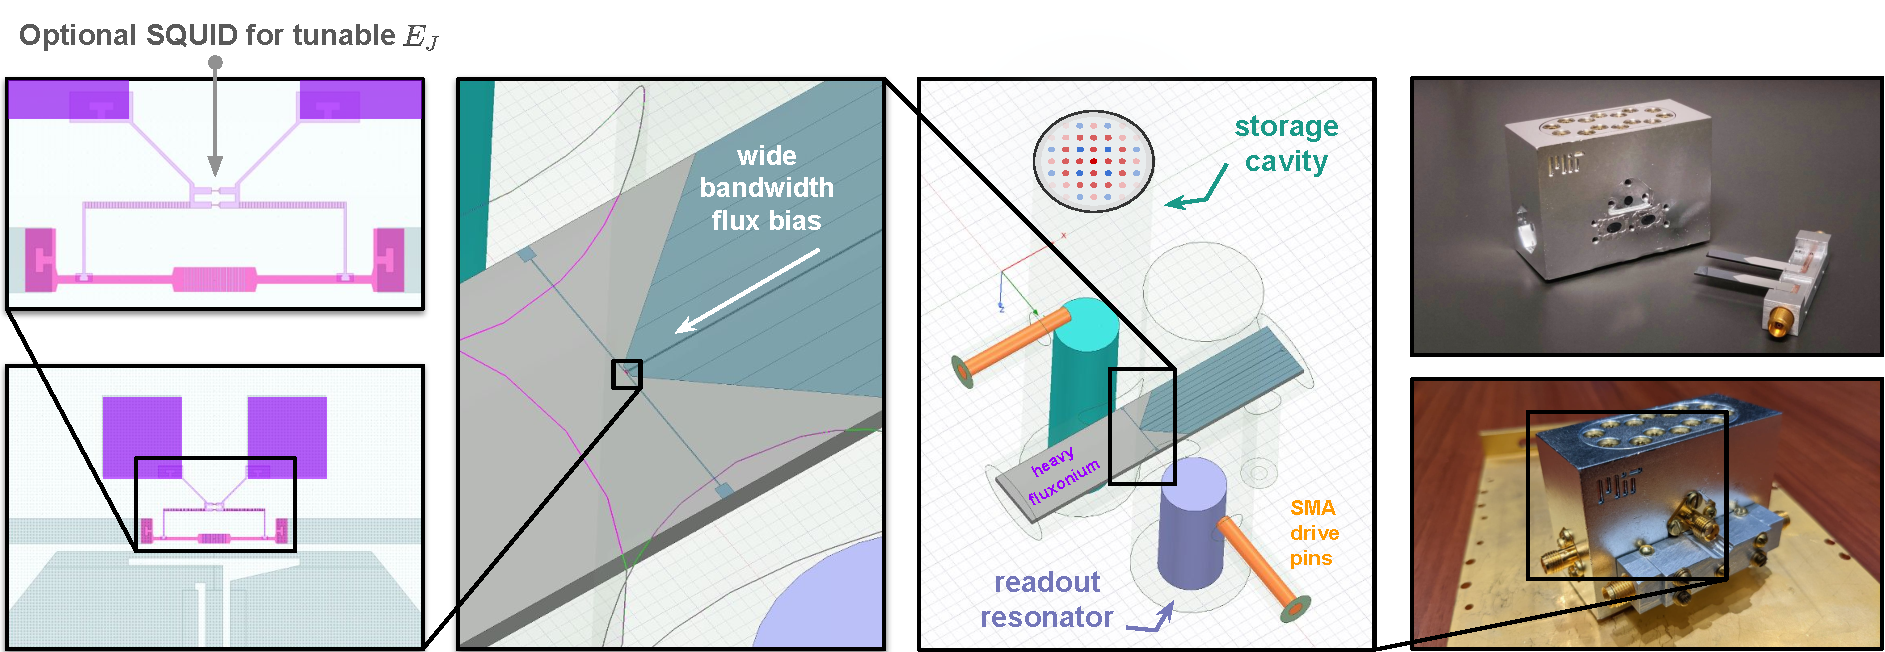
\includegraphics[width=\linewidth]{Figures/4/3DGKP-Schematic.pdf}
    \caption{\todo{Caption}}
    \label{fig:4-3DGKP-schematic}
\end{figure}



\subsection{Cryogenic Setup}

The experiments were performed using a Leiden CF-CS81 dilution refrigerator operated at base temperatures of 8-10 mK. The fridge consists of five temperature stages\footnote{Temperature in the fridge is primarily tracked using three 1 k$\Omega$ platinum (PT-1000) thermometers at the 50K, 3K, and MXC plates, as well as additional capacitive sensors at the MXC. \todo{check!}} as shown in Fig. \ref{fig:4-fridge-wiring}, as well as seven shielding cans that each thermalize to a different temperature stage (not pictured). Specifically, we have two vacuum cans thermalized to room temperature and 1K respectively, and three other cans that provide additional electromagnetic shielding. Finally, to protect against magnetic fields and infrared (IR) radiation, we use two mu-metal shields \todo{check this??} on the coldfinger. A timelapse video of the process to install these cans can be found \href{https://youtu.be/KkvUc9Aw77s?t=829}{here}. 

\begin{figure}[h]
    \centering
    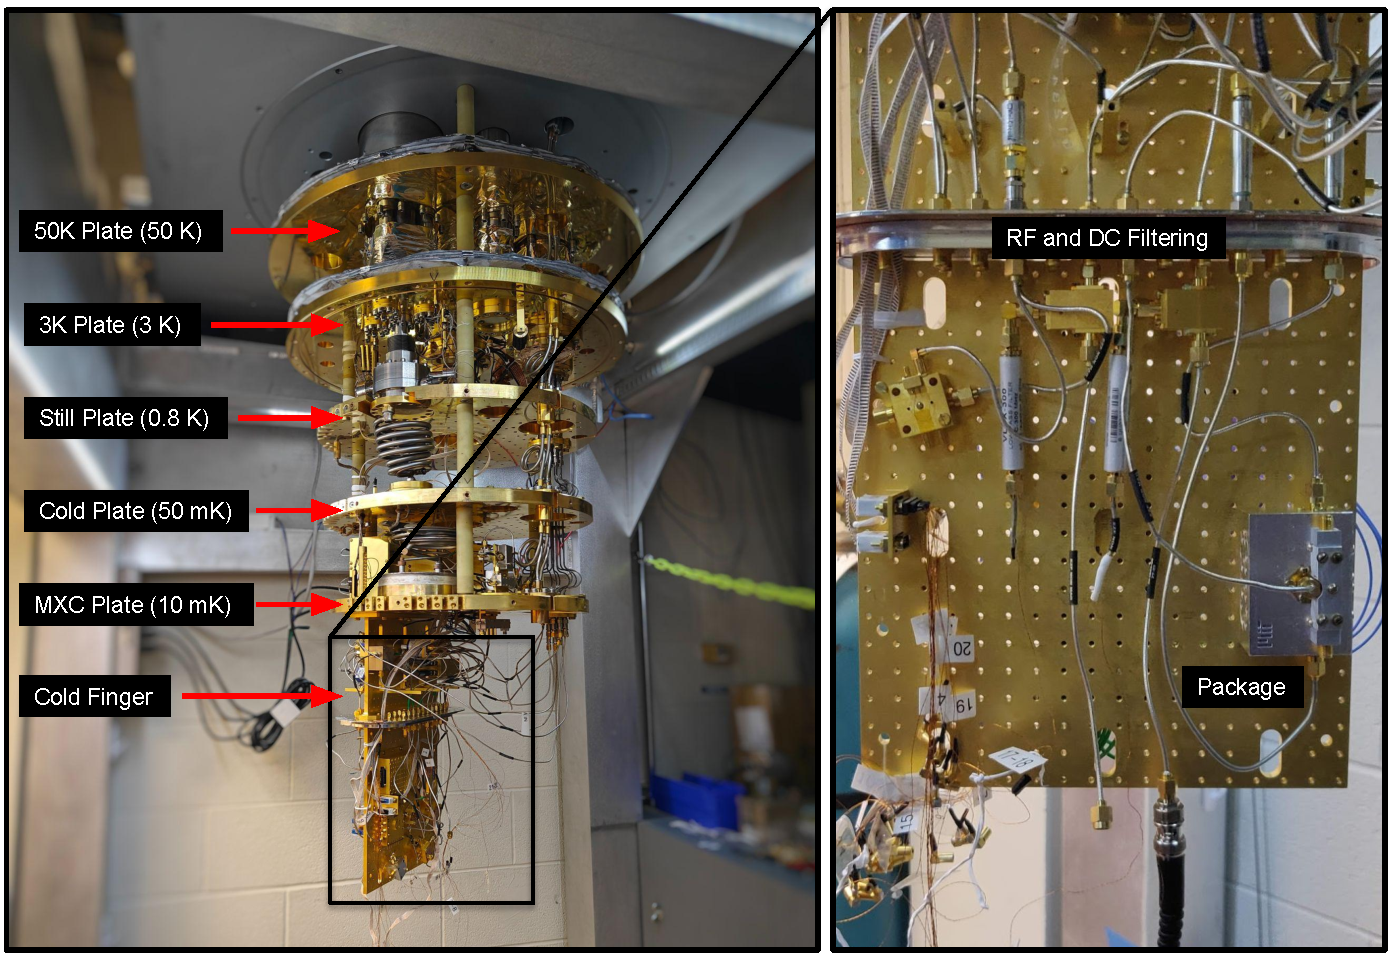
\includegraphics[width=0.9\linewidth]{Figures/4/Fridge-Wiring.pdf}
    \caption{\todo{Caption}}
    \label{fig:4-fridge-wiring}
\end{figure}

The specific experiments presented in this thesis used both DC and radio-frequency (RF) microwave lines to deliver signals to the 3D cavity and fluxonium package. We used three microwave ``drive'' lines for the two fluxonium qubits and the storage resonator, as well as two DC twisted pair connections to provide static flux biasing for the two qubits. The qubit RF and DC signals were first individually filtered and then combined at the mixing chamber through an RF choke. We filtered the DC component using a Mini-Circuits VLFX-300+ low-pass filter, while the RF component was filtered via a K\&L Microwave 12 GHz low-pass filter. This configuration allowed us to probe the higher level transitions of the fluxonium in two-tone spectroscopy through the qubit drive line. 

To attenuate thermal noise coming from the room temperature setup, several attenuators were placed along each of the input microwave lines: a total of 50 dB for the ``drive'' lines and 70 dB for the ``readout'' line. The readout setup had several salient features worth noting: firstly, we used just a single microwave line connected to the two readout cavities via microwave switch; by setting the switch configuration, we selected which of the cavities to measure. Secondly, we used circulators to measure the cavity resonances in reflection. Finally, the reflected output readout signal was pre-amplified using a Josephson travelling wave parametric amplifier (TWPA) at the MXC stage, before being further amplified by a low-noise high-electron-mobility transistor (HEMT) amplifier at 3K, and then a room temperature MITEQ amplifier. The full wiring schematic for this setup is shown below in Fig. \ref{fig:4-microwave-wiring-diagram}. 

\begin{figure}[h]
    \centering
    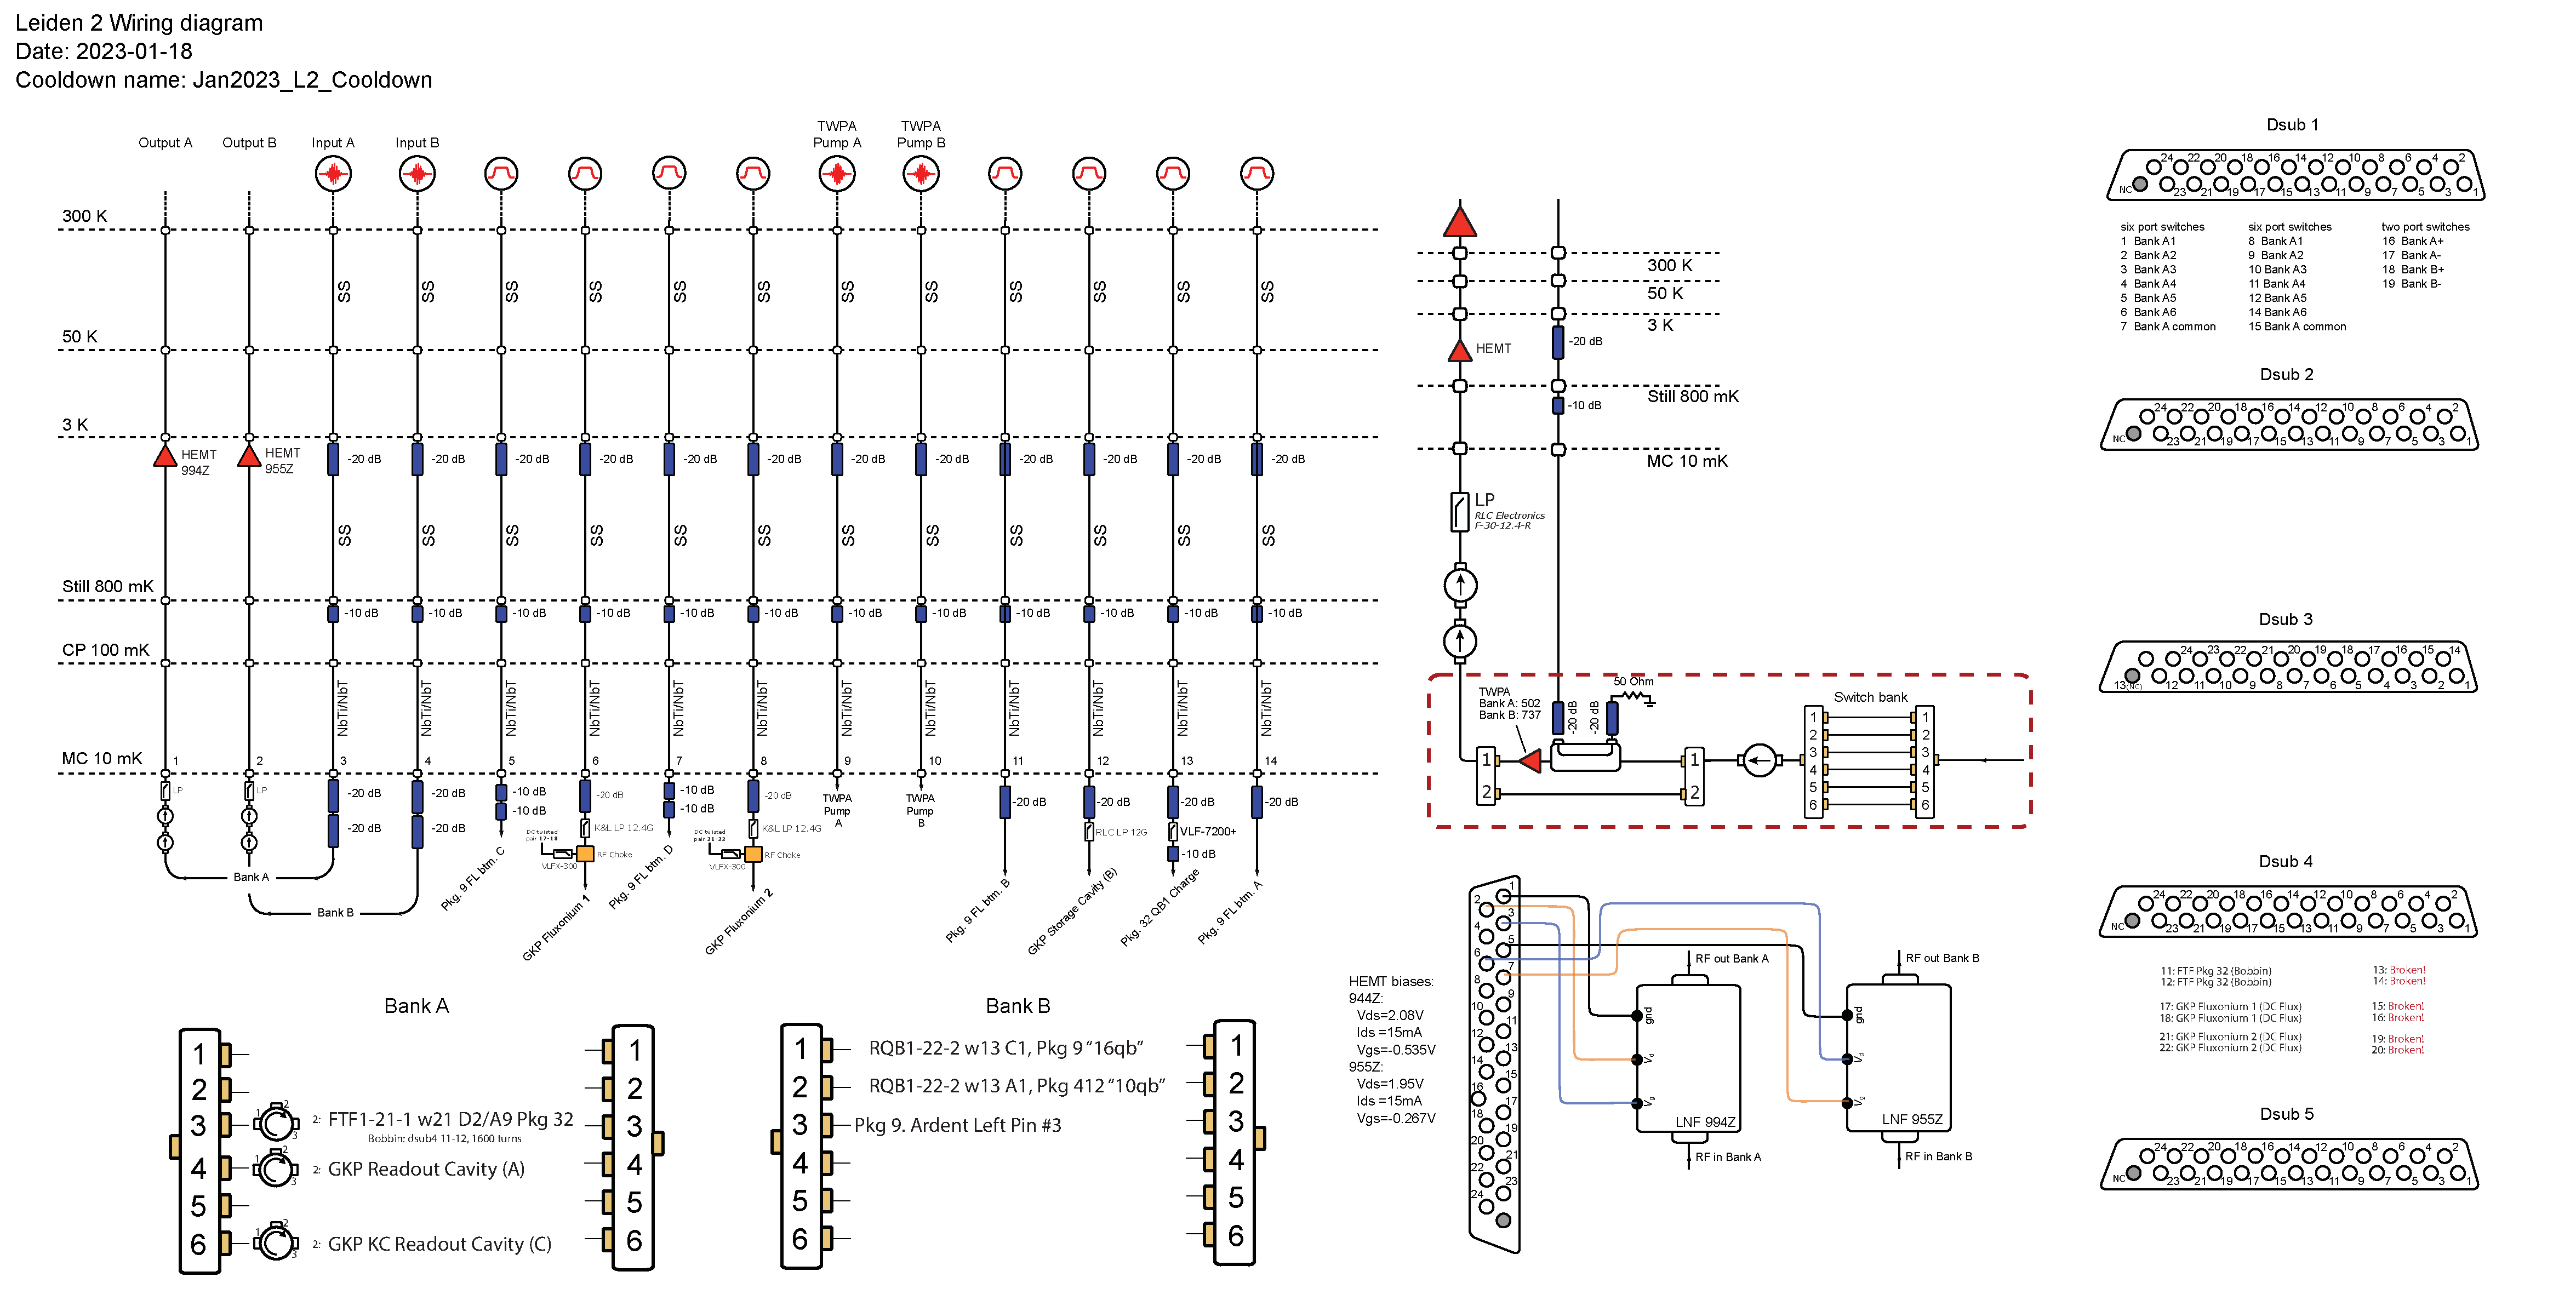
\includegraphics[width=\linewidth]{Figures/4/Microwave-Wiring-Diagram.pdf}
    \caption{\todo{replace image with simplified and corrected version}}
    \label{fig:4-microwave-wiring-diagram}
\end{figure}

At room temperature, pulse waveforms for the various elements were generated using an OPX+ controller from Quantum Machines. For the storage drive, we used an Agilent PSG Signal Generator (E8267D) from Keysight to supply an RF signal which was then combined with the intermediate-frequency (IF) signal from the OPX using the PSG's internal wide-bandwidth IQ mixer. The qubit drive was produced similarly, using a separate Agilent PSG Signal Generator. When performing low-frequency two-tone spectroscopy of the fluxonium $g$--$e$ transition, however, we bypassed the Agilent and instead used baseband signals in the 0-350 MHz range directly from the OPX. Finally, the readout resonator IF signals were generated via the OPX and then passed into a Rohde and Schwarz SGS100A SGMA RF source for upconversion using an internal IQ mixer. The local oscillator (LO) reference signal used for IQ modulation was also passed on to a separate external IQ mixer to demodulate the readout RF output signal coming out of the fridge. The demodulated intermediate-frequency I and Q components were then digitized and processed using the FPGA within the OPX. All microwave signal generators were frequency-locked via a common 10 MHz rubidium clock. 

The DC signals used for static flux biasing were generated via a Yokogawa GS200 Voltage/Current source operated in ``Voltage'' mode; this was then sent into the Qdevil breakout board and then into the fridge via a Fisher cable. Once in the fridge, the signal lines were passed through a resistive DC low-pass filter at the ??K stage \todo{check this!} before terminating in a twisted pair connection. When operating a Yokogawa (or ``Yoko'') in Voltage mode, the DC signal is typically routed through a 1-10 k$\Omega$ resistor to produce an associated current; anecdotally around our lab, this has also been reported to help reduce flux noise from DC lines. However, in the experiments reported below, we mostly chose not to do this and instead used only the bare resistance of the DC line when connected to the fluxonium device, which we measured to be 152.5 $\Omega$ using a multimeter when the fridge was cold. This allowed us to generate a larger current for a given voltage. As we discuss in Sec. \ref{sec:4_Time_Domain}, we later also measured the flux noise amplitude of the qubit when using the ``Current'' mode of the Yoko and found negligible differences in the results. 

\section{Resonator and Two-Tone Spectroscopy}

\textit{In this section, we will present experimental results from our first 3D cavity-fluxonium device with a GKP1 fluxonium chip in our Mark II cavity. We begin with a spectroscopic characterization of the readout resonator and qubit here, followed by time-domain measurements of the qubit in Sec. \ref{sec:4_Time_Domain}, and finally discuss storage resonator measurements in Secs. \ref{sec:4_StorageChi} and \ref{sec:4_StorageCoherenceProblems}. Unless stated otherwise, all data in the upcoming sections was taken using readout cavity A and its associated fluxonium chip. We therefore restrict our focus to the subsystem of the Mark II cavity-fluxonium package comprised of cavity A (readout resonator), fluxonium A (qubit), and cavity B (storage resonator).}

\subsection{Resonator Spectroscopy}
In most circuit QED experiments, the readout resonator forms a crucial gateway through an experimenter probes the system of interest. To this end, the first measurement step we took after cooling down our device was to locate the readout resonator via spectroscopy. As discussed in Sec. \ref{sec:4_3D_Cavity_Resonators}, the readout pin length was chosen here to be overcoupled, with a target coupling rate of $\kappa_c/2\pi \approx 10$ MHz. We were thus able to locate the cavity resonance fairly easily using the VNA and later via pulsed resonator spectroscopy on the OPX with a 10 $\mu$s pulse [see Fig. \ref{fig:4_resonator_spectroscopy}(a)].
\begin{figure}[h!]
    \centering
    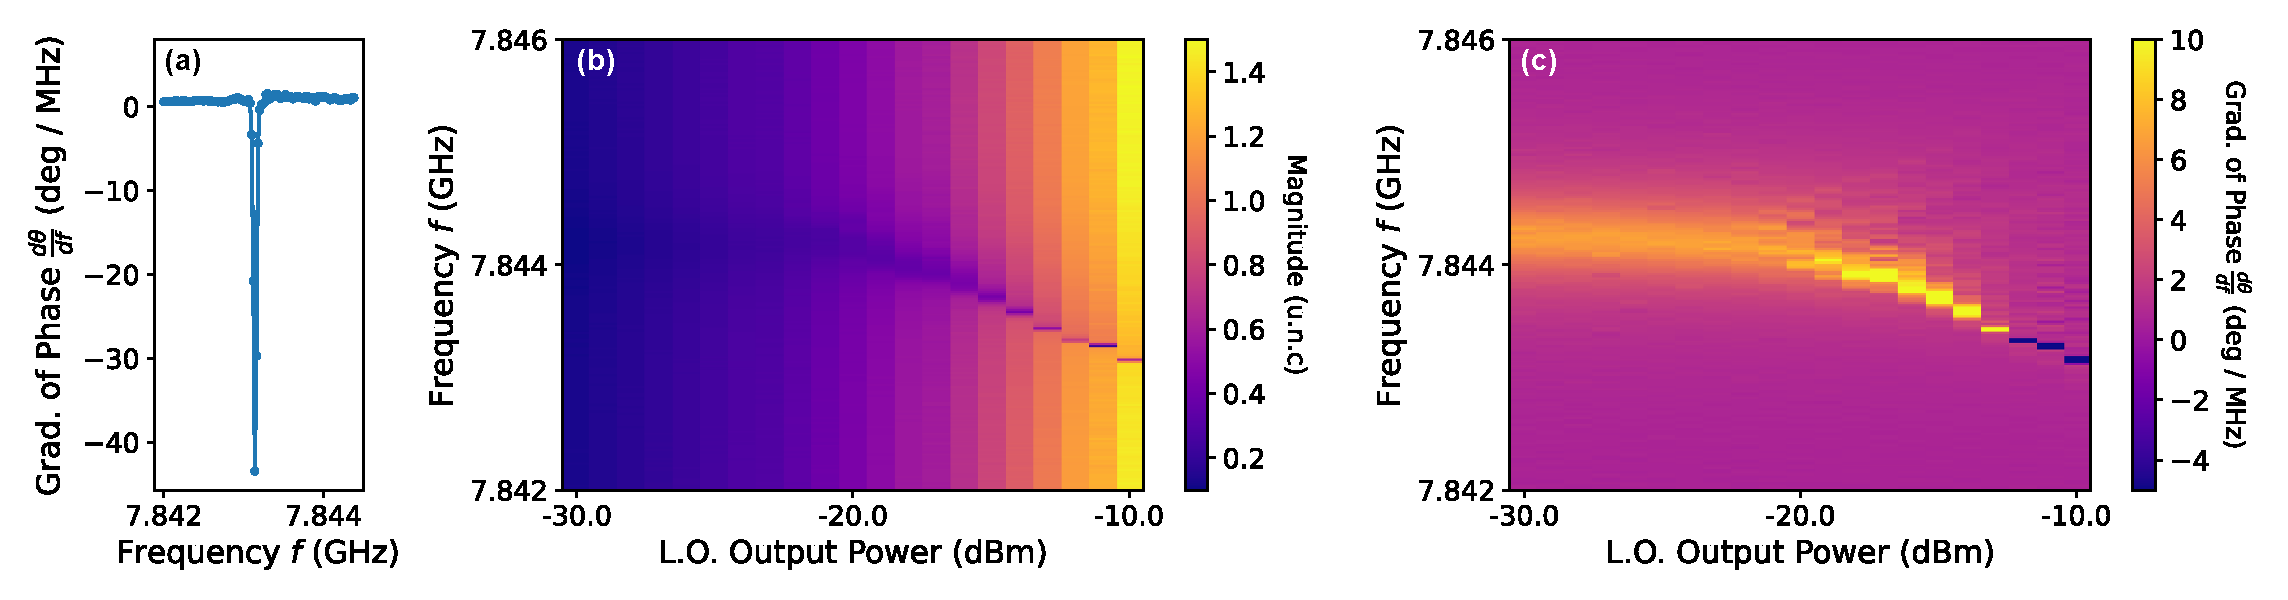
\includegraphics[width=\linewidth]{Figures/4/resonator_spectroscopy.pdf}
    \caption{\textbf{(a)} Readout cavity resonance measured using a time-domain resonator spectroscopy sequence. We plot the gradient of the phase $\theta$ of the reflected signal. \textbf{(b,c)} Sweep of resonator spectroscopy vs. drive power; here we plot both the magnitude and phase.}
    \label{fig:4_resonator_spectroscopy}
\end{figure}

We next repeated pulsed resonator spectroscopy as a function of the input power of the resonator tone to realize a so-called ``punchout'' measurement [Fig. \ref{fig:4_resonator_spectroscopy}(b-c)]. In the data, we observe the resonator ``punching'' out, i.e. its frequency shifting downwards towards its bare value as we increase the drive power and decouple from the nonlinear degrees of freedom in the system (e.g. the qubit or antenna mode here). Punchout is typically used as a way to check whether a qubit is alive, since the nonlinearity of the qubit directly results in a nonlinear response in the resonator. For a practical explanation of this, I refer interested readers to Ref. \cite{naghiloo2019introduction}, which also gives a step-by-step experimentalist's introduction to qubit measurements in circuit QED. 

Due to its coupling to the fluxonium qubit, we also expect the resonator to inherit some flux dependence in addition to nonlinearity. Therefore, after verifying that the resonator frequency changes with power, we next performed resonator spectroscopy vs. the applied external flux bias on the qubit [see Fig. \ref{fig:4_resonator_spectroscopy_vs_flux}]. We set the bias using the room temperature Yokogawa source to set voltage (which induced a current through the DC line, and in turn generated an applied flux through the fluxonium loop). After setting each bias voltage, we waited for 0.1s for the flux to settle and then performed resonator spectroscopy.  

\begin{figure}[h]
    \centering
    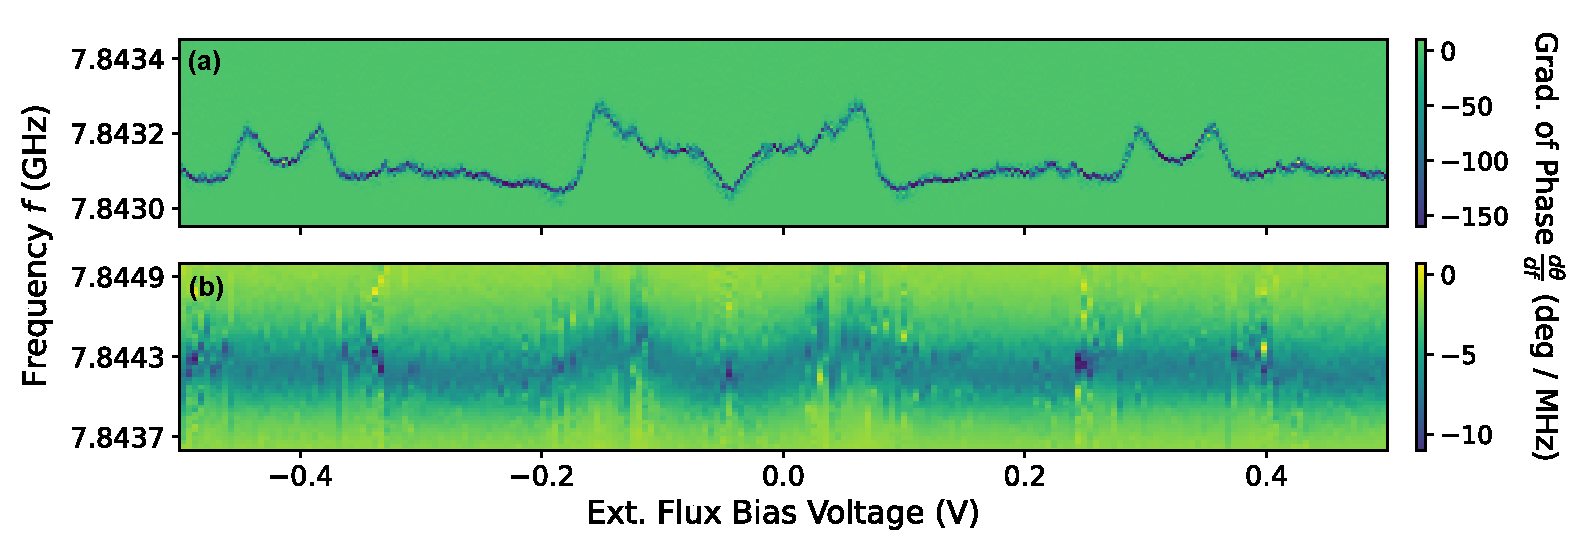
\includegraphics[width=\linewidth]{Figures/4/resonator_spectroscopy_vs_flux.pdf}
    \caption{Resonator spectroscopy vs. external bias voltage on the qubit. The top panel shows high-power data with an LO output power [cf. Fig. \ref{fig:4_resonator_spectroscopy}] of -10 dBm, while bottom panel shows lower-power data taken at -30 dBm. We see the resonator spectrum is indeed periodic with the bias voltage.}
\label{fig:4_resonator_spectroscopy_vs_flux}
\end{figure}

We see that the the resonator frequency indeed varies periodically with the bias voltage. From the periodicity of the spectrum, we found (and later corroborated via qubit two-tone spectroscopy measurements) that a flux quantum in this device corresponds to 4.872 mA, realized in this configuration via a voltage of about 0.743 V applied over the line resistance of 152.5 $\Omega$. The resonator spectrum is expected to be symmetric about both zero external flux ($\Phi_{\rm ext} = 0$) and ``half-flux'' ($\Phi_{\rm ext} = \Phi_0/2$), and we can observe two symmetry points above --- one at $V_b \approx -0.045$ V, and other at both $V_b \approx 0.326$ V and $V_b \approx -0.414$ V. From the averaged data in Fig. \ref{fig:4_resonator_spectroscopy_vs_flux} alone, it is rather difficult to identify which of these symmetry points corresponds to ``half-flux''. However, we can make this identification by instead working with single-shot data, i.e. not directly averaging across shots on the OPX during readout. At $\Phi_{\rm ext} = 0$, the fluxonium has a single ground state $\ket{g}$ that the qubit relaxes to in thermal equilibrium. Thus the dispersive readout will result in a \textit{single} ``I-Q blob'' in the demodulated signal. However, at $\Phi_{\rm ext} = \Phi_0/2$, both the ground and excited states will be thermally occupied in equilibrium due to the low-frequency nature of the qubit \cite{manenti2023quantum}, and thus we expect to see two ``blobs'' in the I-Q plane corresponding to the qubit initial state being in either $\ket{g}$ or $\ket{e}$. When we set the Yoko voltage to $V_b = -0.04465$ V, the single-shot data [cf. Fig \ref{fig:4_single_shots}] reveals two IQ ``blobs'' in the histogram, confirming that this bias point is, in fact, the half-flux sweet spot. (By association the other symmetry points correspond to \textit{integer} flux quanta). Therefore, using our calibration of the flux axis, we can map between the bias voltage and the applied external flux $\Phi_{\rm ext}$ in subsequent measurements. 

\begin{figure}[h]
    \centering
    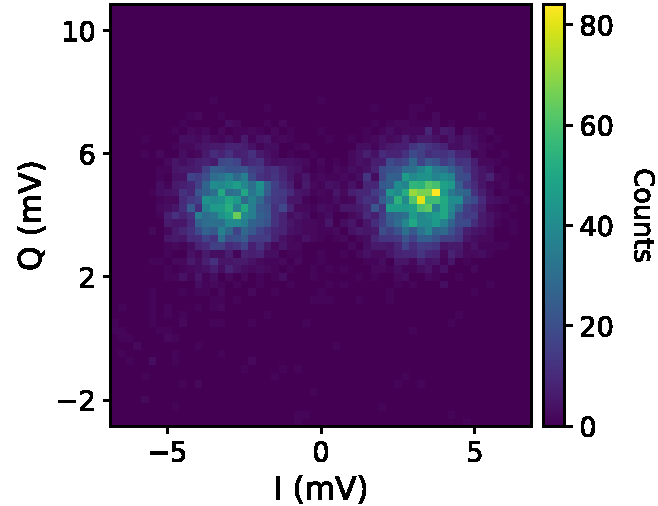
\includegraphics[width=0.6\linewidth]{Figures/4/single_shots.pdf}
    \caption{Histogram of 10,000 digitized single-shot readout measurements, plotted in the I-Q plane. The two ``blobs'' correspond to the two qubit states $\ket{g}$ and $\ket{e}$ that will both be populated in equilibrium when the fluxonium is parked near the half-flux sweet spot.}
\label{fig:4_single_shots}
\end{figure}


\newpage
\subsection{Two-Tone Spectroscopy}
After characterizing the resonator, our next step was \textit{two-tone spectroscopy} (also called qubit spectroscopy). Here, the two ``tones'' in question are (i) a qubit drive tone to probe transitions of the fluxonium, followed by (ii) a resonant readout tone. Practically, we can understand a two-tone spectroscopy experiment as follows by considering the dispersive Hamiltonian \cite{zhu2013cQEDfluxonium}:
\begin{equation}
    \hat{H} = \sum_k \tilde{E}_k \op{k}{k} + \bigg(\omega_r^0 + \sum_k \chi_k \op{k}{k}\bigg) \hat{a}^\dagger\hat{a}
\end{equation}
We have Lamb-shifted qubit energies $\tilde{E}_k$ and eigenstates $\ket{k}$, as well as a resonator whose frequency $\tilde{\omega}_r$ (in parentheses) depends on the qubit state. For the sake of illustration, let's briefly work near zero flux so that only the ground state $\ket{g}$ is initially populated in thermal equilibrium. The basic idea of the experiment is to play a weak continuous spectroscopy (or ``\textit{saturation}'') tone on the qubit. As we sweep the frequency, we'll eventually come into resonance with a qubit transition, e.g. $f_{gl}$ between $\ket{g}$ and some other state $\ket{l}$. When this happens, the resonant tone has the effect of driving Rabi oscillations between the states $\ket{g} \leftrightarrow \ket{l}$; furthermore, over many multiples of the coherence time, the qubit state will also change due to $T_1$ relaxation and/or heating processes. As a result, the qubit will be left in a non-equilibrium (i.e. driven, dissipative) steady state $\hat{\rho}$ with occupation probabilities $p_k$. Due to the dispersive interaction, this mixed state in turn leads to a final average resonator frequency 
\begin{equation}
    \ev{\tilde{\omega}_r}_{\rm final} = \omega_r^0 + \Tr\bigg(\hat{\rho} \sum_k \chi_k \op{k}{k}\bigg) = \omega_r^0 + \sum_k p_k \chi_k
\end{equation}
that is different from the initial one, i.e. $\ev{\tilde{\omega}_r}_{\rm init} = \omega_r^0 + \chi_g$. Using a resonator measurement, we can then detect this change in the resonance frequency (e.g. by measuring the change in signal phase when ``reading out'' at a fixed frequency $\ev{\tilde{\omega}_r}_{\rm init}$), and so map out the qubit transitions. If we now do this as a function of flux, the initial qubit state may also need to be described by a mixed state, e.g. a thermal mixture of $\ket{g}$ and $\ket{e}$ near half-flux; nevertheless, as long as the initial and final mixed states lead to different average resonator frequencies, we will be able to identify that a transition has occurred. 

In experiment, we performed wideband two-tone spectroscopy to map out the higher energy transitions of the fluxonium versus external flux. The full spectrum is shown below in Fig. \ref{fig:4_two_tone_vs_flux_full}, and we already see a rich set of features in the data. The qubit transitions have a clear dependence on flux, and are notably symmetric about the two sweet spots at $\Phi_{\rm ext} = 0$ and $\Phi_{\rm ext} = \Phi_0/2$. In panel (b), we overlay a theoretical prediction obtained from numerical diagonalization of the fluxonium Hamiltonian with free parameters $E_C$, $E_J$, and $E_L$. We extract
\begin{equation}
    E_C/h \approx 1.678 \,\, \text{GHz}, \quad  E_J/h \approx 8.987 \,\, \text{GHz}, \quad  E_L/h \approx 0.342 \,\, \text{GHz} 
    \label{eq:4_qubit_parameters_fit}
\end{equation}
as the qubit parameters for this device by fitting to the data. This is within the range that we designed for, and results in a qubit frequency of approximately 94.1 MHz at half-flux. 

At this resolution, there are also certain features that appear to be constant with flux. We can identify these are the various linear modes in the system, e.g. the storage resonator at 8.86 GHz, and the two on-chip antenna modes at 8.60 GHz and 8.46 GHz. Since each of these modes has a dispersive shift to the readout resonator (also shown), we are able to see them in this two-tone measurement just as we do the other qubit transitions\footnote{We can also see some other faint qubit-like transitions near half-flux. We'll comment on these later, as they are actually quite interesting: it turns out that they are two-photon ``parasitic'' qubit-resonator transitions.}. Note that each of these linear modes (including the readout) has \textit{some} flux dispersion if we zoom in close enough. This is important for readout calibration, as typically the readout frequency must be calibrated at each new flux operating point. In the data shown here, we did not do this, and instead used a constant frequency tone at 7.8442 GHz, which was approximately resonant across the entire flux range (cf. low-power data in Fig. \ref{fig:4_resonator_spectroscopy_vs_flux}). While this worked reasonably well, we nonetheless see variations in readout constant that could be improved by first redoing resonator spectroscopy at each flux point prior to two-tone, or by creating a lookup table ahead of time. 

From the wideband spectrum (also cf. Fig. \ref{fig:4_two_tone_vs_flux_zoom} below), we can clearly see that the storage resonator frequency lies between the two sets of fluxonium plasmon transitions. This is precisely the condition we had hoped to engineer in our system: as a reminder, we refer to it as bosonic mode threading. 

\begin{figure}[htp]
    \centering
    \includegraphics[width=0.88\linewidth]{Figures/4/two_tone_vs_flux_full.pdf}
    \caption{\textbf{(a)} Wideband two-tone spectroscopy data showing a landscape of transitions in our 3D-cavity package. \textbf{(b)} Overlaid fitted theoretical predictions based on numerical diagonalization of the fluxonium Hamiltonian with 3 free parameters: $E_C$, $E_J$, $E_L$. Various linear modes such as the storage, readout, and antennas are plotted as straight lines.}
\label{fig:4_two_tone_vs_flux_full}
\end{figure}
\clearpage

\begin{figure}[hp]
    \centering
    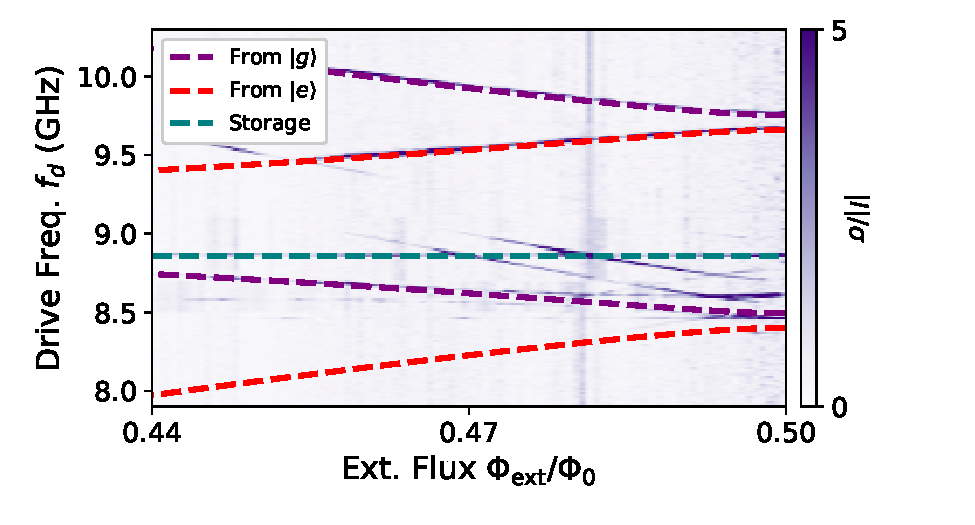
\includegraphics[width=0.8\linewidth]{Figures/4/two_tone_vs_flux_zoom.pdf}
    \caption{Zoomed-in two-tone spectroscopy showing bosonic mode threading, with the storage resonator frequency in between the two sets of fluxonium plasmon transitions. Dashed lines from $\ket{g}$ and from $\ket{e}$ show theoretical predictions from numerical diagonalization of the qubit, as before. The storage flux dispersion cannot seen at this resolution.}
\label{fig:4_two_tone_vs_flux_zoom}
\end{figure}

Our next experimental step was low-frequency qubit spectroscopy near half-flux using a direct baseband drive to map out the qubit  $\ket{g}\to\ket{e}$ transition: we show the data below in Fig. \ref{fig:4_qubit_spectroscopy}. Unlike prior measurements, here we used a dual readout post-selection scheme \cite{ding2023FTF} to improve contrast and assign an occupation probability to the qubit. This was crucial to obtain our results, and we will discuss it further in the upcoming section.

\begin{figure}[!b]
    \centering
    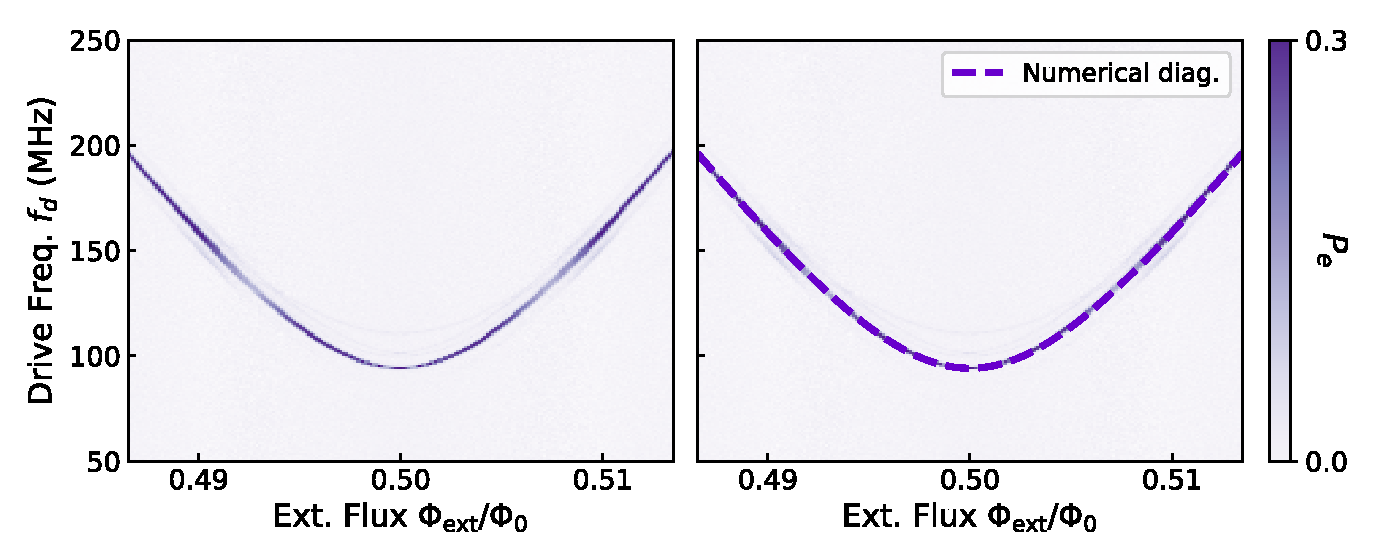
\includegraphics[width=0.9\linewidth]{Figures/4/qubit_spectroscopy.pdf}
    \caption{Post-selected baseband two-tone spectroscopy showing the fluxonium $\ket{g}\to\ket{e}$ transition with and without the theoretical fit from numerical diagonalization using the same parameters as before [Eq. \eqref{eq:4_qubit_parameters_fit}]. At half-flux, the qubit frequency is 94.1 MHz.}
\label{fig:4_qubit_spectroscopy}
\end{figure}

\section{Time-Domain Measurements of the Qubit \label{sec:4_Time_Domain}}

\subsection{Post-Selection via Single-Shot Readout}

Near half-flux, the energy of the fluxonium qubit transition $\h\omega_q$ can be much smaller than the ambient temperature $k_BT$ of a typical dilution refrigerator. As a result, the fluxonium in equilibrium will be in a thermal mixture of $\ket{g}$ and $\ket{e}$; we saw this in Fig. \ref{fig:4_single_shots} already. For our specific parameters of $f_q = 94.1$ MHz and $T = 9$ mK, the excited state population is given by a Boltzman distribution: $p_e \simeq 1 / (e^{\h\omega_q/k_B T} + 1) \approx 60\%$. For the higher-level (i.e. wideband) two-tone spectroscopy above, this initial thermal distribution was not a problem --- on the contrary, starting from a mixed state is even beneficial, allowing us to see transitions out of both $\ket{g}$ and $\ket{e}$. However, for baseband qubit spectroscopy probing the $\ket{g}\leftrightarrow\ket{e}$ transition, and critically also for time-domain experiments, this ceases to be true. For these measurements, we instead want to be able to discriminate between the two states. In our experiments, the approach we chose to do this was single-shot readout and post-selection. We specifically followed the dual readout scheme discussed in Refs. \cite{ding2023FTF, ding2023thesis} (cf. Fig. \ref{fig:4_postselection} below)\footnote{At this point, I'd also sincerely like to thank Leon Ding for his early guidance with fluxonium experiments!}. Here, the first readout pulse initializes the fluxonium state to either $\ket{g}$ or $\ket{e}$ via projective measurement. We then start the rest of the experimental sequence (e.g. qubit pulses, delays, storage pulses) from a known initial state, and finally conclude with a second readout pulse to record the qubit state. All the time-domain measurements that follow used this post-selected sequence. 

\begin{figure}[b!]
    \centering
    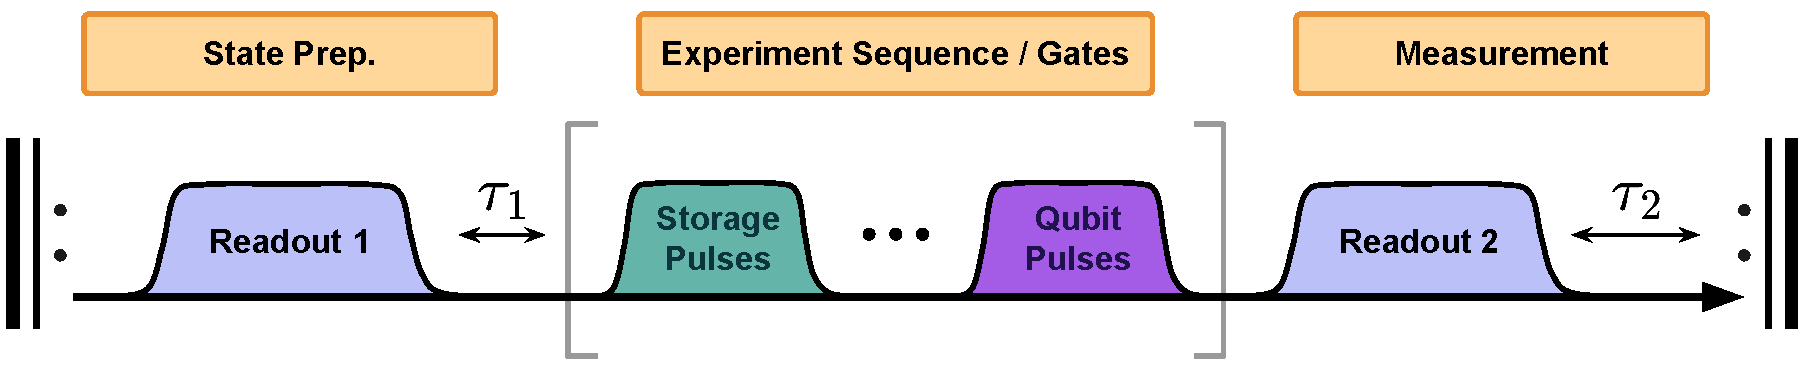
\includegraphics[width=0.9\linewidth]{Figures/4/postselection.pdf}
    \caption{Dual readout post-selection. Here, the first readout prepares the qubit in $\ket{g}$ or $\ket{e}$ and the second readout records the final qubit state after performing the experiment sequence. We introduce a short ring-down time $\tau_1$ to allow readout photons to decay after the first readout, and a longer delay $\tau_2$ to let the qubit relax to equilibrium between shots.}
    \label{fig:4_postselection}
\end{figure}
\clearpage

\subsection{Rabi Oscillations and Pi Pulse Calibration}

After having identified the qubit frequency in two-tone spectroscopy, we next turned to time-domain experiments involving coherent manipulation of the qubit state. The first of these was, of course, to demonstrate Rabi oscillations between the $\ket{g}$ and $\ket{e}$ states using a resonant drive. In heavy fluxonium, the $T_1$ protection that arises due to the small charge matrix element also has the effect of making it generically more difficult to drive the associated transitions. As a result, several previous experiments with fluxonium or other low-frequency flux qubits have had to use either non-adiabatic Landau-Zener flux control \cite{oliver2005mach, campbell2020universal, zhang2021universal}, or virtual (Raman) transitions mediated by a higher energy state \cite{earnest2018realization}. Thankfully, we were able to use more conventional microwave-based control via a resonant drive, since our device was not quite so heavy. 

In Fig. \ref{fig:4_rabi}, we show a typical \textbf{power Rabi} measurement, taken with the qubit parked at half-flux. For this data, we specifically used a fixed length ($\tau = 200$ ns) Gaussian pulse whose amplitude we swept to generate Rabi oscillations: this is shown below on the left for a resonant drive. Meanwhile, on the right, we have a characteristic ``chevron'' plot. By finding the point of minimum contrast in the 2D sweep of Rabi frequency and amplitude, we can tune up $\pi$- and $(\pi/2)$-pulses on the qubit. 

\begin{figure}[h]
    \centering
    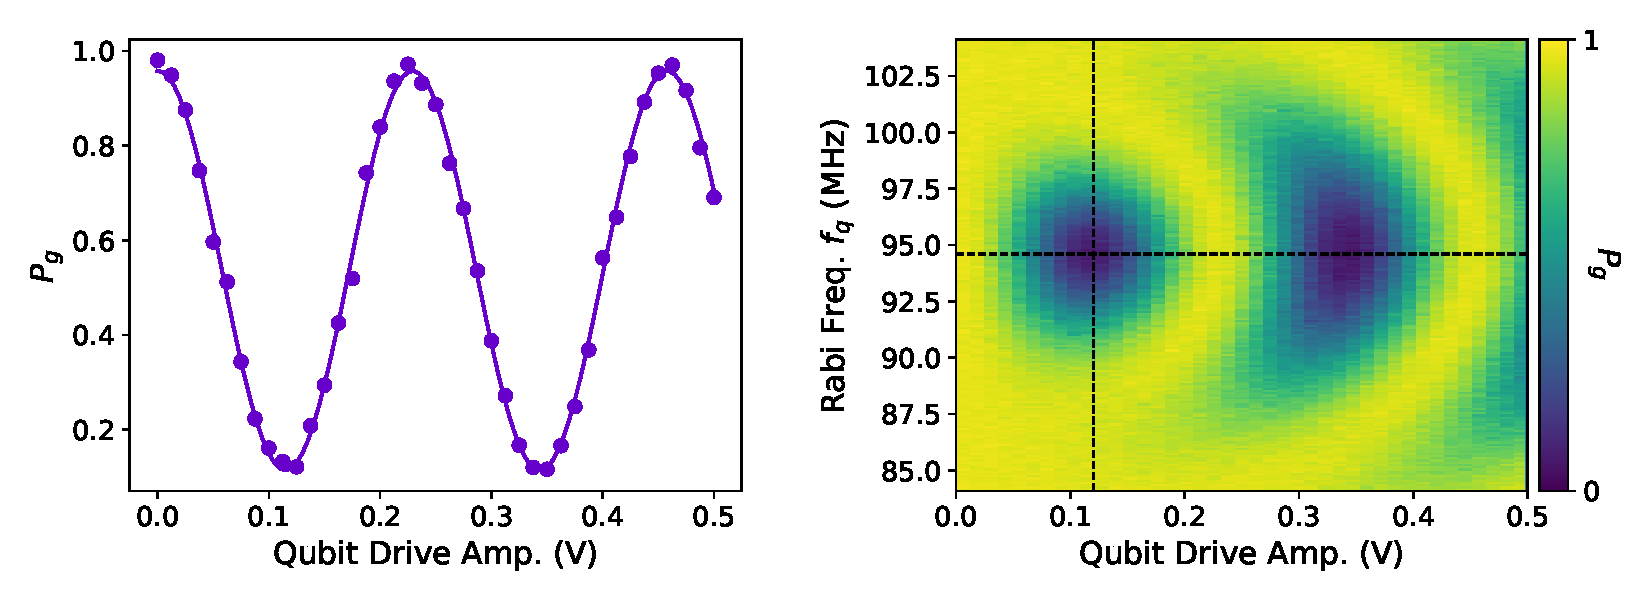
\includegraphics[width=0.95\linewidth]{Figures/4/rabi.pdf}
    \caption{Left: Power Rabi experiment showing characteristic Rabi oscillations as we sweep the qubit drive amplitude for a resonant pulse. Right: we can sweep the frequency to get a ``chevron'' plot; we can use the minimum contrast point to tune up a $\pi$-pulse.}
    \label{fig:4_rabi}
\end{figure}

In subsequent measurements, we typically tuned up two kinds of $\pi$-pulses: the first was a shorter $\tau = 48$ ns pulse, which we used in most of the time-resolved qubit experiments. The second was a ``selective'' qubit pulse, of length $\tau = 2.4$ $\mu$s, chosen so that the associated spectral bandwidth of the pulse $1/\tau$ was smaller (at least at half-flux) than the dispersive shift $\chi$ between the qubit and storage mode (cf. Sec \ref{sec:4_StorageChi} where we discuss this further). We also later switched from Gaussian to cosine pulses; the latter were easier to work with due to their well-defined end points (zero amplitude at the start and end of the pulse). 

\subsection{Measuring the Fluxonium \texorpdfstring{$T_1$}{T1}\label{sec:4_fluxonium_T1}}

Our next set of experiments involved measuring the $T_1$ relaxation time of the fluxonium. The post-selection sequence we used to realize the measurement consists of two readouts separated by a variable length delay. The first readout initializes the qubit in either $\ket{g}$ or $\ket{e}$, while the second is used to track a change of state. The result is a characteristic $T_1$ relaxation curve showing an exponential decay of the qubit populations with time. We show an example of such a curve in Fig. \ref{fig:4_qubit_T1_vs_flux_single}(a), from which we extract a decay constant $T_1 = 220 \pm 10$ $\mu$s. Panel (b) shows the results of the same experiment now repeated across various external flux biases: we see that the flux-dependence of the qubit $T_1$ is very sharply peaked and symmetric about half-flux, with a maximum value of $T_1 \approx 265$ $\mu$s.

\begin{figure}[h]
    \centering
    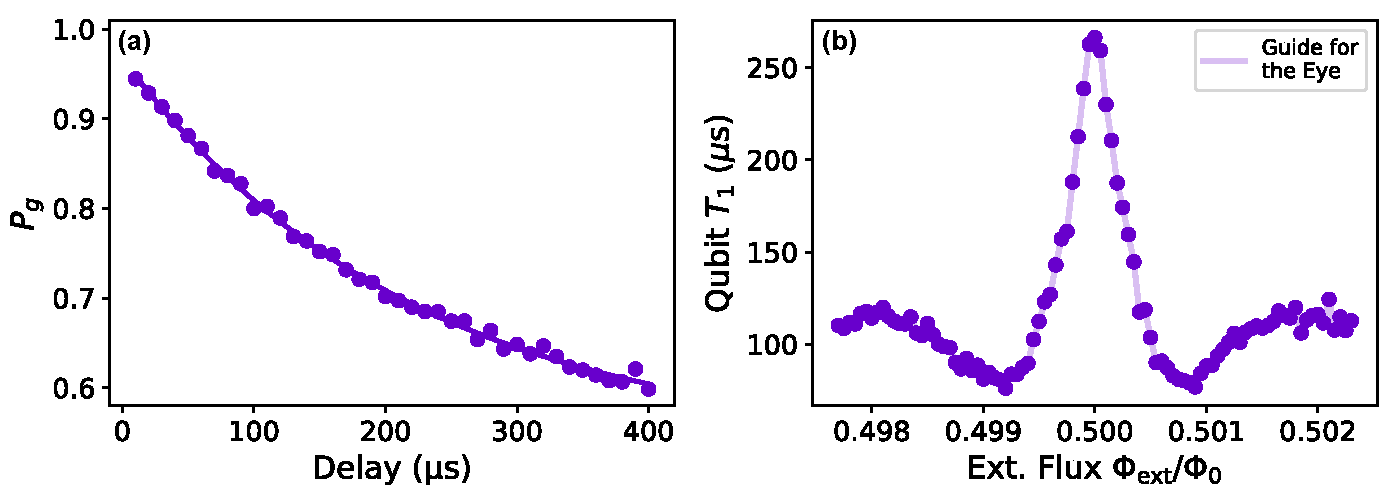
\includegraphics[width=0.95\linewidth]{Figures/4/qubit_T1_vs_flux_single.pdf}
    \caption{\textbf{(a)} $T_1$ experiment measuring qubit population $P_g$ vs. time. Solid line shows a fit to an exponential decay with an extracted $T_1 = 220 \pm 10$ $\mu$s. \textbf{(b)} Sweep of $T_1$ experiments vs. flux; at each flux, we tune up a $\pi$-pulse and then measure the $T_1$ decay.}
    \label{fig:4_qubit_T1_vs_flux_single}
\end{figure}

The sharply peaked flux-dependence in Panel \ref{fig:4_qubit_T1_vs_flux_single}(b) was one of the first experimental mysteries that we encountered with this device. For the parameters of our fluxonium, and assuming a capacitive (i.e. dielectric) loss model, we naively expected $T_1$ to improve away from half-flux. There are other loss models that would predict $T_1$ degrading away from half-flux (e.g. quasiparticle tunneling); however, we were unable to reproduce the sharp initial drop-off in any numerical simulations at the time of the experiment. [As we discuss below, however, we have since come up with a model that we believe may explain these observations]. 

If we go out even further in flux, we see an even richer structure to the flux-dependence of the fluxonium $T_1$ [see Fig. \ref{fig:4_qubit_T1_vs_flux_spec}]. Away from half-flux, we see a clear drop in $T_1$, followed by an apparent revival around $\Phi_{\rm ext} \approx 0.485\Phi_0$. However, as we move leftwards, we again see further drop-offs in the $T_1$. Although these observations puzzled us for some time, we eventually came to the hypothesis that the drop-offs in $T_1$ may be a form of Purcell decay.

\begin{figure}[h]
    \centering
    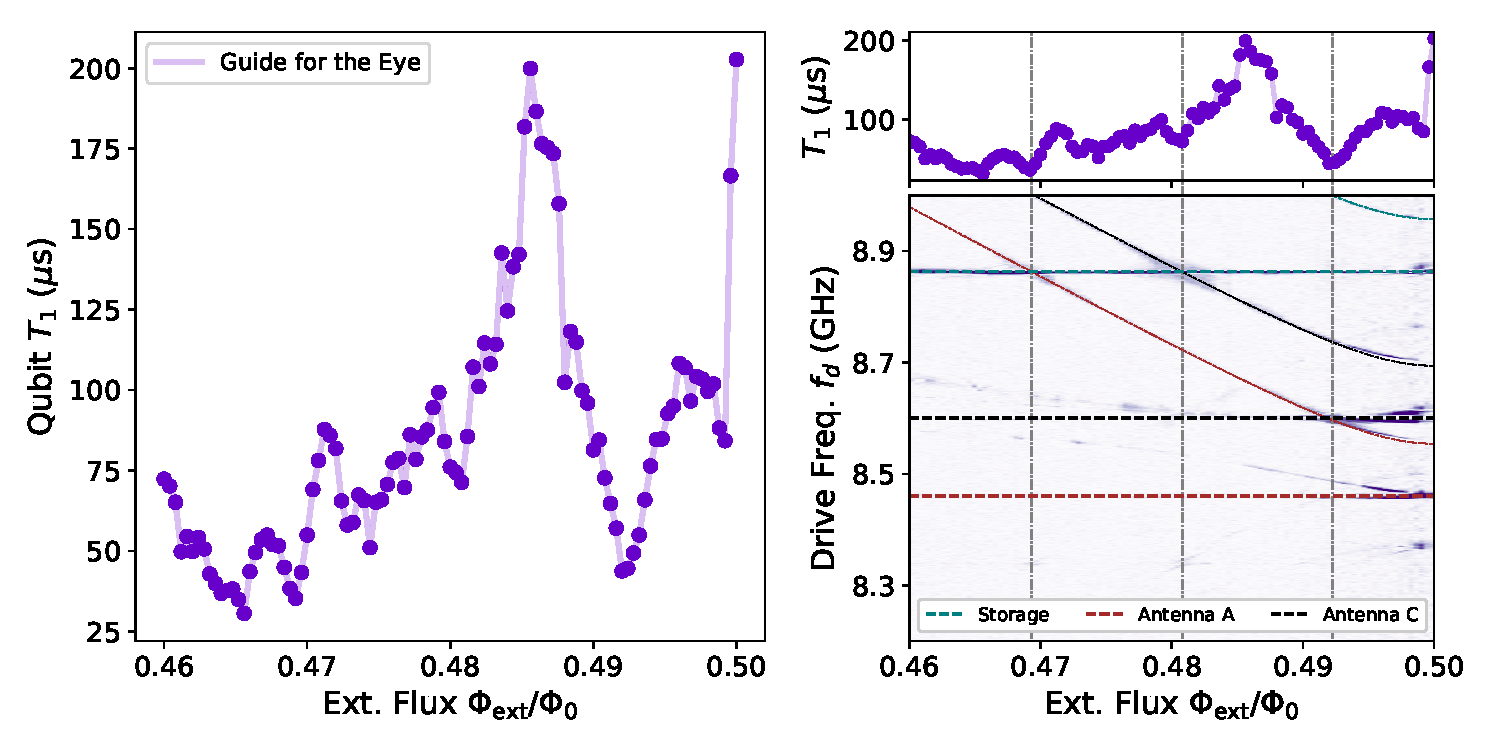
\includegraphics[width=0.95\linewidth]{Figures/4/qubit_T1_vs_flux_spec.pdf}
    \caption{Left: Sweep of $T_1$ experiment vs. flux over a wider range of external fluxes. We see rich structure, which we associate with accidential two-photon resonances in the spectrum. Right: we match the locations of the largest qubit $T_1$ drops to two-tone spectroscopy, showing that they coincide with the resonances shown. See main text for details.}
    \label{fig:4_qubit_T1_vs_flux_spec}
\end{figure}

In the right panel of Fig. \ref{fig:4_qubit_T1_vs_flux_spec}, we reproduce the $T_1$ data from the left panel, but also now align it with two-tone spectroscopy data taken earlier. At this resolution, the storage and the two antenna modes are straight lines. On top of these we see certain flux-dependent transitions: it turns out that these are ``two-photon'' transitions! (We showed these in Fig. \ref{fig:4_two_tone_vs_flux_full} as well). Specifically, they correspond to the frequencies of the linear modes \textit{plus} the qubit $\ket{g}\to\ket{e}$ frequency, i.e. they are activated when $\omega_d \approx \omega_{\rm lin} + \omega_{ge}$ where $\omega_{\rm lin}$ can be the frequency of the storage or either antenna. Intuitively, we can understand the drop-offs in qubit $T_1$ occurring when this ``two-photon'' transition is tuned into resonance with one of the \textit{other} linear modes. For example, at $\Phi_{\rm ext} \approx 0.48\Phi_0$, we have $\omega_{\rm C} + \omega_{ge} \approx \omega_{s}$, and at $\Phi_{\rm ext} \approx 0.47\Phi_0$, we have $\omega_{\rm A} + \omega_{ge} \approx \omega_{s}$. In both cases, the resulting resonance leads to a direct Purcell-type decay of the qubit. We have since been able to reproduce this behavior using numerical Purcell simulations, including the initial drop-off at half-flux shown in Fig. \ref{fig:4_qubit_T1_vs_flux_single}; although the latter does not correspond to a direct resonance, we suspect it arises as a higher order term in perturbation theory. I will leave a full investigation of this effect to future work. 

\subsection{Ramsey and Echo Measurements}

We also performed coherence measurements of the qubit using typical $T_2$ Ramsey and Echo sequences. A Ramsey measurement involves applying two ($\pi/2$)-pulses separated by a variable delay $\tau$; by detuning the frequency of the pulses from qubit frequency, we observe characteristic Ramsey oscillation fringes of the qubit population vs. time with a frequency given by the detuning. An Echo measurement is similar, but adds an additional $\pi$-pulse in the middle of the sequence to refocus dephasing errors; in this case, all pulses are set to be resonant with the qubit and we see no oscillations. In both cases, we fit to an overall decay envelope of the form $\exp[-(\tau/T_2)^{1 +\alpha}]$, corresponding to Markovian dephasing and $1/f^\alpha$ flux noise. We show some typical Ramsey and Echo measurements in Fig. \ref{fig:4_T2_ramsey_echo} taken for the qubit parked at half-flux.

\todo{Perhaps mention flux noise amplitude if there is space for it.}

\begin{figure}[h]
    \centering
    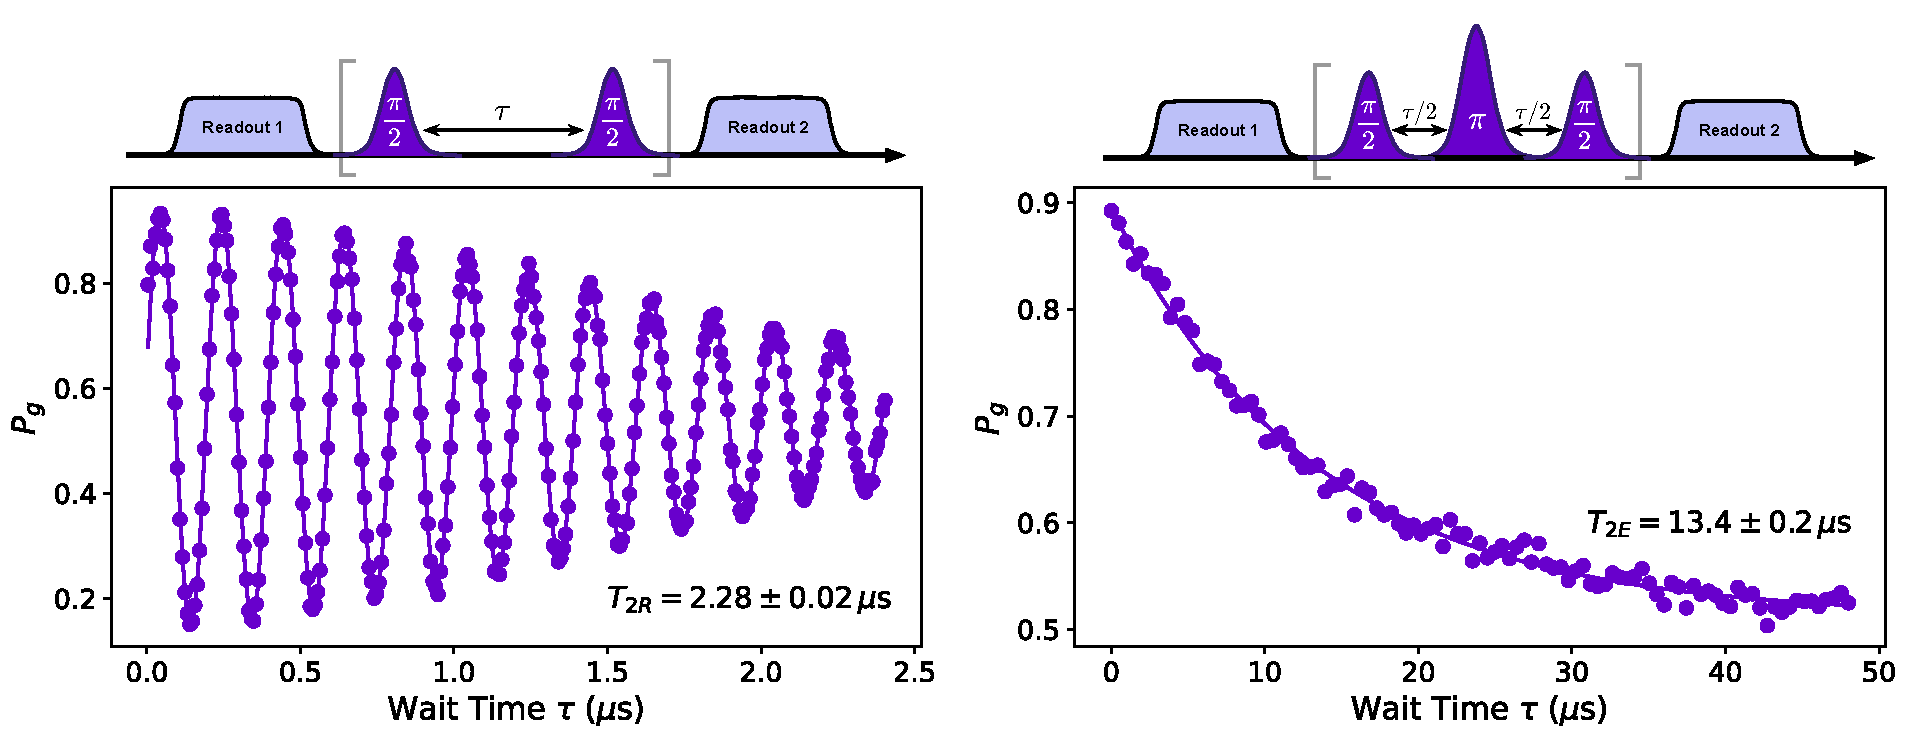
\includegraphics[width=0.95\linewidth]{Figures/4/T2_ramsey_echo.pdf}
    \caption{$T_2$ Ramsey and Echo measurements for our fluxonium at half-flux.}
    \label{fig:4_T2_ramsey_echo}
\end{figure}

\clearpage
\section{Storage Resonator Measurements \label{sec:4_StorageChi}}

\subsection{Storage Spectroscopy}

We are now ready to discuss measurements of the storage resonator. At this stage, we had already identified the storage in two-tone spectroscopy, and now wanted to corroborate this using a storage spectroscopy experiment. This measurement uses the qubit as a meter to probe the storage resonator frequency; as shown below in Fig. \ref{fig:4_storage_spectroscopy}, it involves driving the storage resonator and then performing a frequency-selective $\pi$-pulse on the qubit. This $\pi$-pulse is chosen to have length $\tau \gg 1/\chi_{qs}$ and a frequency that corresponds to the qubit frequency when the storage has zero photons. When the initial storage drive is resonant with the cavity, it will displace the storage away from the vacuum $\ket{0}$; as a result, the $\pi$ pulse fails. Only when the storage drive is off-resonant will the cavity remain in its $\ket{n=0}$ state, and thus cause the $\pi$-pulse to be implemented correctly. Finally, given our need for post-selection here, we can initialize the fluxonium in either $\ket{g}$ or $\ket{e}$ to see two different resonance dips. In practice, we used a constant $\tau = 2.4$ $\mu$s for the selective pulse.
\begin{figure}[h]
    \centering
    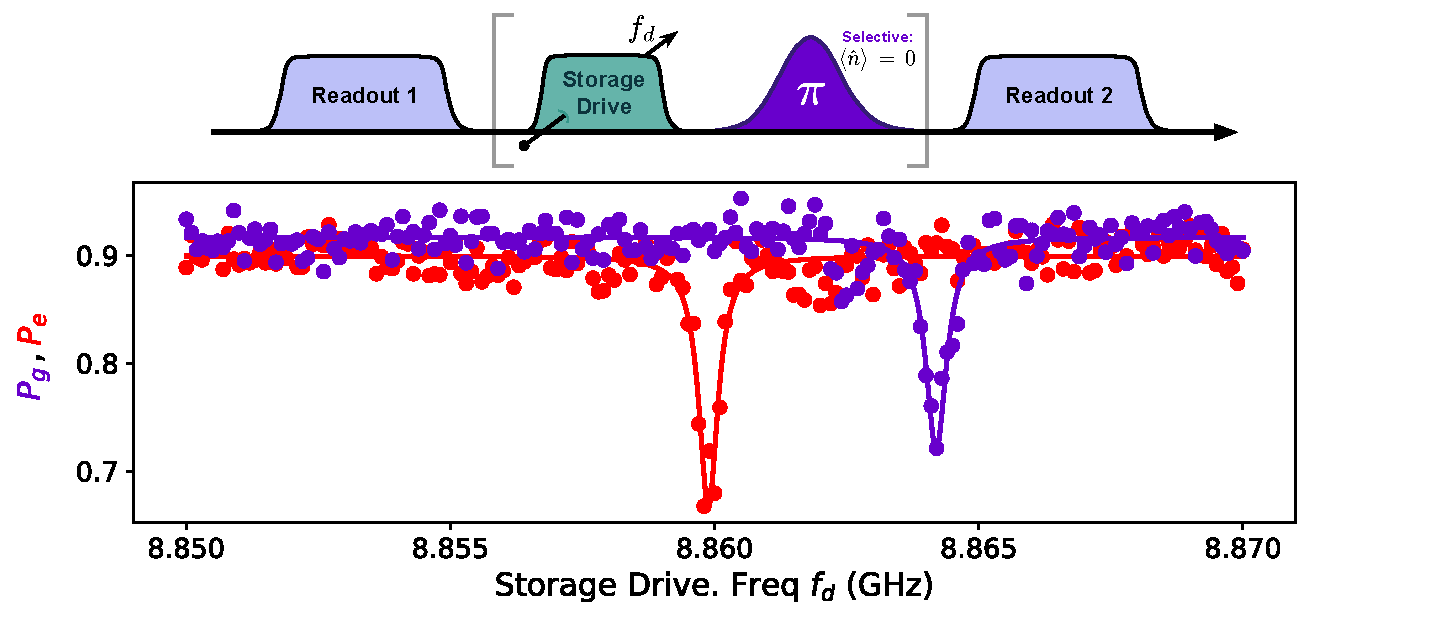
\includegraphics[width=0.85\linewidth]{Figures/4/storage_spectroscopy.pdf}
    \caption{Storage spectroscopy measurement via the qubit. This experiment enables us to determine the storage frequency when the qubit is in $\ket{g}$ or $\ket{e}$ respectively.}
    \label{fig:4_storage_spectroscopy}
\end{figure}

\subsection{Engineering a Tunable Dispersive Shift}

The storage spectroscopy measurement above presents a method to extract the dispersive shift $\chi_{qs}$ between the fluxonium and storage. We simply sweep the external flux $\Phi_{\rm ext}$ and tune up a frequency-selective $\pi$-pulse at each bias point. Since the storage flux dispersion is minimal, we can perform a storage spectroscopy at each flux, and calculate $\chi_{qs}$ as the difference in the resonance frequency when the qubit is in $\ket{g}$ vs. $\ket{e}$, as is consistent with a Hamiltonian coupling term $\chi_{qs} \hat{a}^\dagger\hat{a}\sigmaz/2$. The result of this measurement is shown in Fig. \ref{fig:4_tunable_chi}, and we see that the dispersive shift indeed tunes with flux and crosses through zero, as is expected with bosonic mode threading. 

\begin{figure}[h]
    \centering
    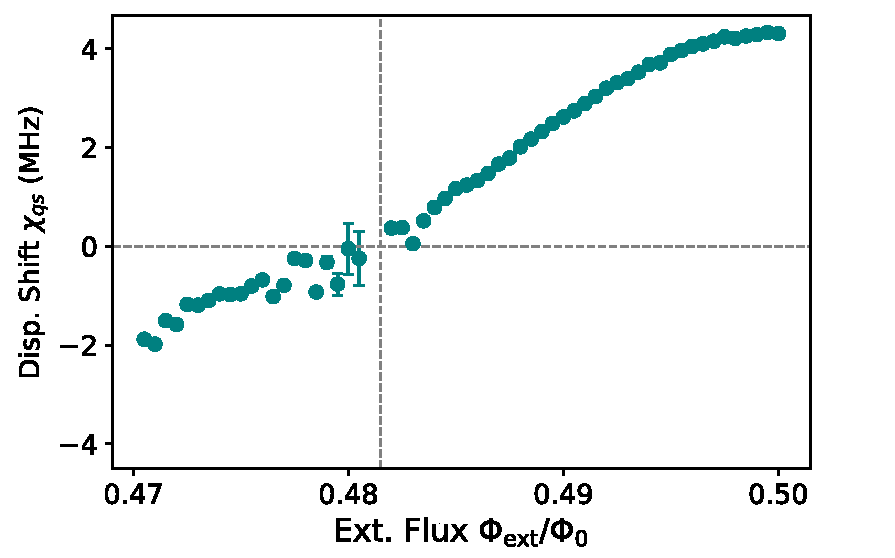
\includegraphics[width=0.6\linewidth]{Figures/4/tunable_chi.pdf}
    \caption{Measurement of the tunable storage dispersive shift $\chi_{qs}(\Phi_{\rm ext})$ vs. the external flux $\Phi_{\rm ext}$. We mark the approximate zero crossing point, which occurs at $\Phi_{\rm ext} \approx 0.481\Phi_0$.}
    \label{fig:4_tunable_chi}
\end{figure}

\noindent Since we used a selective $\pi$-pulse of the same length $\tau = 2.4$ $\mu$s at each flux point, we don't expect this method to work well near the zero crossing point where $\chi_{qs} \to 0$ since there the condition $\tau \gg 1/\chi_{qs}$ ceases to hold. We consequently see slightly larger error bars at the crossing and cannot measure the exact point at which $\chi_{qs}=0$ (the fit fails). 

\clearpage

\section{Storage Coherence: Problems and Pitfalls \label{sec:4_StorageCoherenceProblems}}

Our next experimental step was to characterize the coherence of the storage resonator. As we later discovered, however, the storage lifetime was severely limited in our device. This led to a series of A/B tests and many months of debugging before we realized that the problem was in some sense inherent to our design. In this section, we will present some of the major clues that led us to this conclusion. 

\subsection{Initial Time-Domain Measurement}

The first method we took to measure the storage lifetime was based on a number-splitting spectroscopy experiment \cite{schuster2007resolving}. This measurement sequence uses a selective qubit $\pi$-pulse, and in particular consists of playing a storage drive at one of the storage peaks (e.g. $\omega_s^{\ket{g}}$) and then performing qubit spectroscopy with the selective pulse. If we post-select to have started with the qubit in $\ket{g}$, then this will enable us to see multiple resonance peaks in the qubit spectrum corresponding to the photon number distribution in the cavity after it is excited via the storage pulse. We can see an example of this on the left plot in Fig. \ref{fig:4_storage_T1_numsplit} below, which shows the photon number distribution (teal) after driving the storage with a 10 $\mu$s pulse, followed by a 2.4 $\mu$s selective qubit $\pi$-pulse. The distribution is specified via the depth of the various resonance dips, and is expected to follow a Poisson distribution as the storage is driven to a coherent state. We contrast this with the case when the storage pulse is not played (grey), resulting in just a single qubit spectroscopy dip corresponding to the storage having $\ket{n=0}$ photons. 

In order to measure the storage $T_1$ this way, we can introduce a variable delay between the storage drive pulse and the qubit $\pi$-pulse. During this time, the storage will experience photon loss $\kappa_{1s}\mathcal{D}[\hat{a}]$ and thus the number distribution will decay back down towards the vacuum. We can measure this decay by parking at, say, the $\ket{n=0}$ dip and recording the change in contrast vs. time. For single-photon loss rate $\kappa_{1s}$, we expect an initial coherent state $\alpha_0$ to decay as $\alpha(t) = \alpha_0 e^{-\kappa_{1s}t/2}$, i.e. so that $\bar{n}(t) = |\alpha(t)|^2 =  \bar{n}_0 e^{-\kappa_{1s}t}$ with $\bar{n}_0 = |\alpha_0|^2$. We can fit the decay of the $\ket{n=0}$ qubit spectroscopy dip by weighting $\bar{n}(t)$ via the Poisson distribution evaluated at $n = 0$. This gives us a fit function $P_{g, 0}(t) = 1-a\cdot\exp[-\bar{n}_0 e^{-\kappa_{1s}t}]$ for the decay, where $a$ is a scale parameter to account for the partial contrast. From this, we can extract the lifetime $T_{1s} = 1/\kappa_{1s}$. We show the result of such a measurement in the right panel of Fig. \ref{fig:4_storage_T1_numsplit}.
\begin{figure}[h]
    \centering
    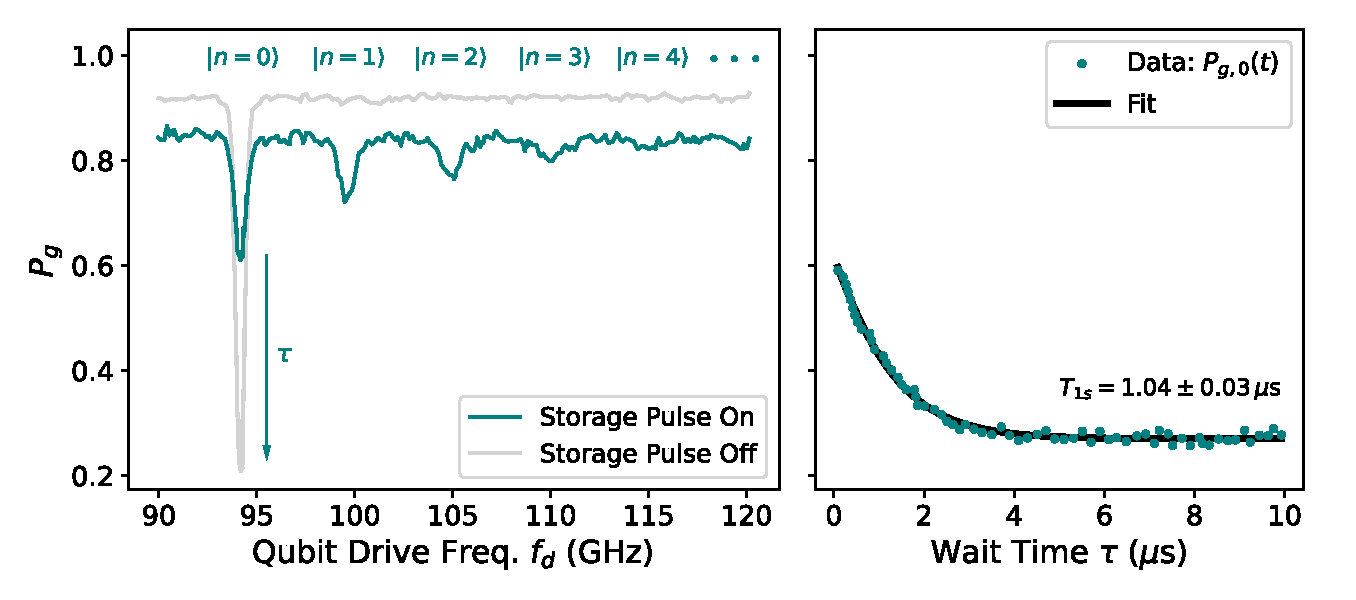
\includegraphics[width=\linewidth]{Figures/4/storage_T1_numsplit.pdf}
    \caption{Left: Number-splitting spectroscopy data for the qubit at half-flux, showing multiple photon-resolved dips (teal) after driving the storage for 10 $\mu$s. If we add a variable delay after the storage pulse, we observe the number distribution decaying back towards the case when the storage has $\ket{n=0}$ photons (grey). Plotting the depth of the $\ket{n=0}$ dip vs. time allows us to measure the single-photon decay and extract the storage lifetime.}
    \label{fig:4_storage_T1_numsplit}
\end{figure}

\subsection{Testing and Progress}
We were very surprised to measure a storage lifetime of $T_{1s} \approx 1$ $\mu$s, given the bare lifetime of the Mark II storage cavity of $T_{1s}^{\rm bare} \approx 740$ $\mu$s that we had seen previously without qubit chips. We therefore set out to debug this part of our system over several subsequent cooldowns. In time, we were able to verify that our bare 3D cavity resonators indeed had high coherence; we tested both the Mark II and Mark III cavities in various configurations as shown in Fig. \ref{fig:4_3D_Cavity_Debugging}. These tests also helped us rule out excess coupling loss due to the storage drive pin. One observation we made is that even inserting blank Si chips into the cavity seemed to degrade their lifetime (i.e. with no qubit, flux line, or metallization). We attributed this to the lossy single-side polished Si wafer that was used to fabricate the fluxonium chips. Nonetheless, this effect alone was not enough to account for the drop in cavity lifetime from over 700 $\mu$s to $\sim\!1$ $\mu$s. 

\begin{figure}[t]
    \centering
    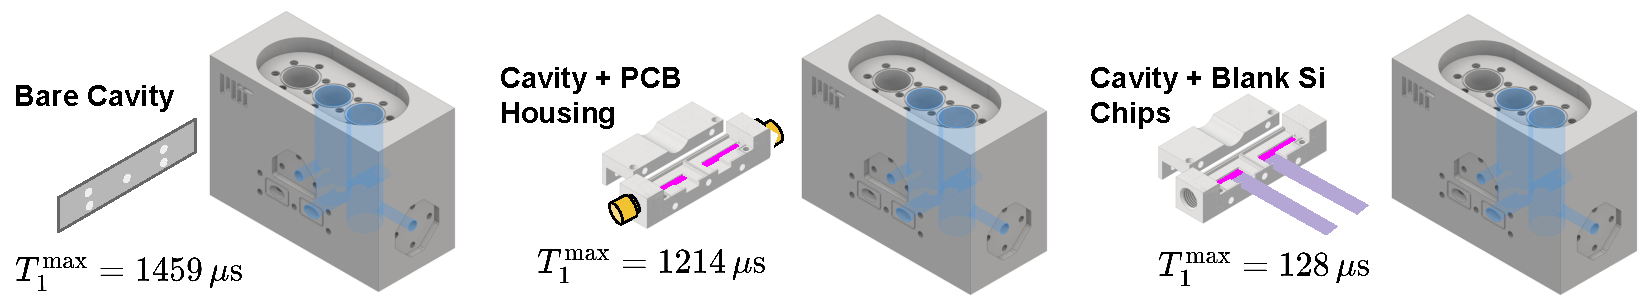
\includegraphics[width=\linewidth]{Figures/4/3D_Cavity_Debugging.pdf}
    \caption{Maximum single-photon $T_{1s}$ measured across all three resonator in the Mark III cavity. Each configuration was tested during a different cooldown of the fridge.}
    \label{fig:4_3D_Cavity_Debugging}
\end{figure}

Our main suspicion was that the storage loss was coming primarily from the qubit flux line; we thus first attempted to remedy it by adding external DC/RF filtering to our lines. Unfortunately, this is did not seem to solve the problem. We later also attempted capping the flux line with a 50 $\Omega$ terminator and then went as far as fully de-wirebonding it; neither of these changes helped appreciably and the storage lifetime remained around 1 $\mu$s or less. Our conclusions from these tests were also muddied by uncontrolled factors between the various cooldowns (e.g. statistical variations in lifetime, degradation of the cavities with time, or changes to the exact amount of indium used in the seals). 

\subsection{Direct Measurement of Loss from the Flux Line}

We were ultimately able to confirm our suspicions about the flux line loss by performing a direct reflection ($S_{11}$) measurement of the 3D cavities \textit{through} the flux lines. We connected a VNA to the flux line and were able to measure the storage cavity resonance, which alone was enough to tell us that the flux line was too strongly coupled (cf. Fig. \ref{fig:4_storage_loss_thru_flux_line}); we ideally should not be able to see anything. Here, however, the low-power resonator spectroscopy measurement shows two dips associated with the fluxonium being in $\ket{g}$ or $\ket{e}$ respectively. To reflect this, we fitted the data to a double Lorenztian $S_{11}$ model consisting of two weighted peaks with identical linewidths but different frequencies. From here, we were able to extract $\kappa_c/2\pi = 320.9$ kHz and $\kappa_i/2\pi = 2.03$ MHz. 

\begin{figure}[h]
    \centering
    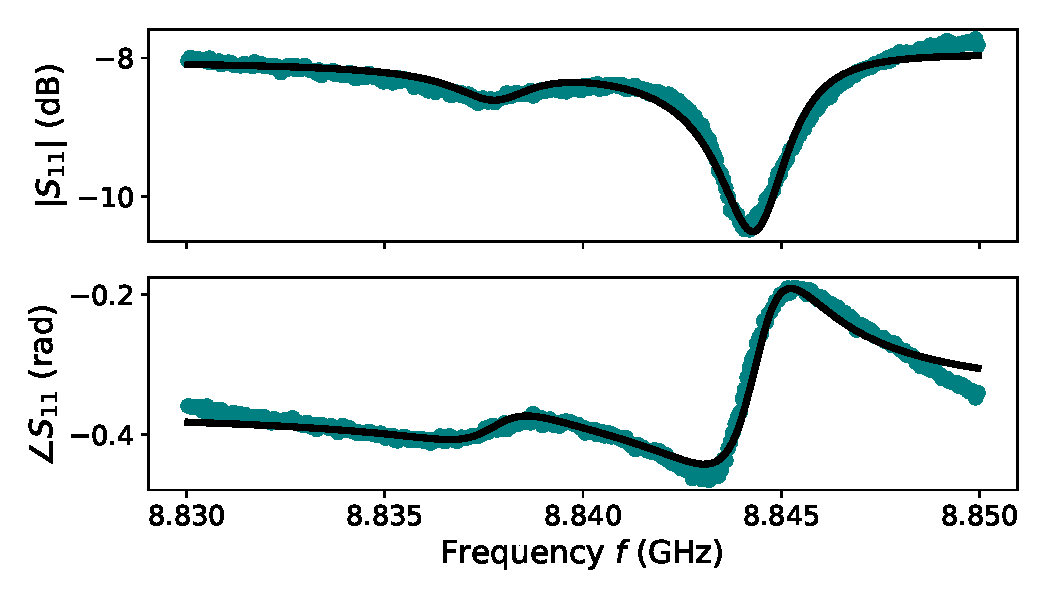
\includegraphics[width=0.7\linewidth]{Figures/4/storage_loss_thru_flux_line.pdf}
    \caption{Direct measurement of the storage resonance through the qubit flux line. At half-flux, we see two peaks associated with the states $\ket{g}$ and $\ket{e}$. We fit data to a double Lorentzian $S_{11}$ model with two weighted peaks of identical linewidth to extract $\kappa_c$ and $\kappa_i$.}
    \label{fig:4_storage_loss_thru_flux_line}
\end{figure}

In the configuration of measuring $S_{11}$ through the flux line, the constant $\kappa_c$ tells us how much of the total storage loss comes from its coupling to the flux line. We get $T_{1c} = 1/\kappa_c \simeq 0.496$ $\mu$s, thus confirming that the flux line is limiting. However, in this measurement, we found that the internal loss $\kappa_i$ is even larger than $\kappa_c$, suggesting there is \textit{another} loss channel at play beyond just the flux line. 

\subsection{Storage Loss HFSS Simulations and Summary}

We were finally able to resolve the storage loss question by revisiting our E\&M eigenmode simulations of the 3D cavity package using Ansys HFSS\footnote{I'd like to thank R\'eouven Assouly for his insight to re-run the simulations, for various tips for using HFSS, and his help and willingness to brainstorm creative solutions during this turbulent time in the project.}. We found that the storage losses were significant even in simulation and thus inherent to our design. This is ultimately the reason why many of the steps we took during our A/B testing did not improve the cavity lifetimes. We show an example simulation in Fig. \ref{fig:4_HFSS_Simulation}, here characterizing the effect of 50 $\Omega$ loss from the flux line [panel (a)]. We consistently found that when the fluxonium chip is inserted, the electric field of the storage mode does \textit{not} stay confined to the post cavity, but instead `leaks out' and does so in two distinct ways: (i) through the qubit flux line, as shown in panel (d), and (ii) by participating in the ground plane mode between the chip and the tunnel walls, as is depicted in panel (e). We saw the former in our measurement of storage loss down the flux line. The latter effect, however, is more subtle and arises when a voltage develops between the metallization of the ground plane and the chip tunnel wall, giving rise to a $(\lambda/4)$-like mode of the entire ground plane. The storage participates in this mode and thus its field can be thought to `leak' down the tunnel. In turn, the storage will experience a full litany of loss mechanisms that 3D cavities are otherwise supposed to be resilient to (e.g. seam loss at the mouth of the tunnel and mode participation in lossy glue and/or PCB dielectrics) \cite{reagor2013reaching,brecht2015demonstration,reagor2016quantum}. We corroborated this in simulation by later including seam loss explicitly. 

\begin{figure}[t]
    \centering
    \includegraphics[width=0.8\linewidth]{Figures/4/HFSS_Simulation.pdf}
    \caption{\textbf{(a)} HFSS model of our 3D cavity-fluxonium device with a 50 $\Omega$ loss channel. \textbf{(b, c)} Exact and approximate models for the tip of the flux line. \textbf{(d)} Eigenmode simulation result showing storage cavity electric field; the field is mostly concentrated around the post cavity, but also leaks down the flux line. \textbf{(e)} Different angle showing the cavity field also participating in the ``ground plane'' mode, and thus leading down the chip tunnel.}
    \label{fig:4_HFSS_Simulation}
\end{figure}

From these simulations, we realized that the `ground plane' loss channel (ii) will always arise if there is significant metallization inside the chip tunnel. While this could in principle be alleviated by somehow grounding the chip to the tunnel wall (e.g. using indium), doing so would necessarily also introduce seam losses, and thus it is not immediately clear how to proceed. Meanwhile, the `flux line' loss (i) could be solved in several ways, e.g. by using some form of on-chip microwave filtering \cite{pozar2012microwave} (more discussion of this in Ch. \ref{ch:5_2DGKP}). We even found in simulation that the shape of the flux tine tip seemed to affect the storage loss significantly [cf. Fig. \ref{fig:4_HFSS_Simulation}(b-c)]; in particular, using the exact shape of the flux line in Fig. \ref{fig:4_HFSS_Simulation}(b), we found $T_{1s} \simeq 0.5$ $\mu$s in simulation, whereas the approximate shape in Fig. \ref{fig:4_HFSS_Simulation}(c) resulted in $T_{1s} \simeq 1.9$ ms. 

In summary, we learned from our experiments that it is a difficult technical challenge to integrate a fast flux line in 3D while maintain the coherence of an otherwise high-Q cavity. Although this presents a major hurdle for using fluxonium in a 3D-cavity architecture for the purpose of bosonic QEC, there are potential paths forward. We will discuss a few such approaches in the upcoming chapter. 

\printbibliography[heading=subbibliography, title = References]
\printbibliography[heading=subbibliography, title = References]
\clearpage
% % ------------------------------------------------

% %%%%% Chapter 5: Next Steps and 2D GKP %%%%%%
\chapter{Next Steps and Moving to 2D\label{ch:5_2DGKP}}


In the previous chapter, we presented the results of our experiments with a fluxonium in a 3D cavity. We demonstrated a tunable dispersive shift between the qubit and the storage resonator via bosonic mode threading and characterized the various components of our system. In doing so, we discovered that the lifetime of the storage mode was \textit{significantly} lower than expected (as compared to its bare value) whenever the qubit chip was inserted into the resonator package. After many rounds of experimentation and testing, we were ultimately able to attribute this effect to two main sources: (i) the storage mode's coupling to the lossy qubit flux line; and (ii), its participation in spurious modes of the 3D superconducting package. While the former issue could in principle be solved via clever microwave engineering and filtering, the latter unfortunately is intrinsic to our 3D design and not easily remedied. As we came to learn, it is generally difficult to integrate fast-flux into a 3D cavity while also maintaining the cavity coherence. 

There are certain approaches that have been proposed and implemented in the literature that work towards integrating fast-flux in 3D. One such example is the magnetic hose from Refs. \cite{gargiulo2021fast,valadares2023demand}. Here, the authors route flux from an external coil to a tunable transmon qubit in a 3D superconducting package using a ``hose'' composed of concentric aluminium and mu-metal layers. In the experiment of Ref. \cite{valadares2023demand} specifically, this is done for the purpose of bosonic cQED, and the authors demonstrate that the lifetime of their 3D storage resonator is not limited by their flux delivery mechanism. Unfortunately, however, the design and implementation of a magnetic hose is quite painstaking, and would require a full redesign of both the cavities and the fluxonium chips that were presented in Ch. \ref{ch:4_3DGKP}. Other designs have also been proposed recently, e.g. Ref. \cite{hutin2024monitoring} or Ref. \cite{maiti2024ancilla}, which both rely on some form of on-chip distributed-element microwave filtering to prevent losses from the flux line at the frequency of the storage. Despite requiring more advanced microwave engineering in design, these approach seem promising for integrating fast-flux in 3D while maintaining the storage resonator lifetime. 

In our case, however, after discovering the root cause of our storage coherence issues and identifying various avenues to proceed from there, we decided to forgo the 3D architecture entirely. This was in part due to the time and difficulty of implementing fast-flux delivery in 3D (which, as highlighted above, is a difficult project in of itself); but it was also a choice we made consciously, motivated by the idea of moving our experiments to 2D. Over the course of our 3D-GKP project, we ended up developing an entirely separate but novel way to do GKP error correction in 2D, using a microwave-activated coupler to generate faster conditional displacements. This 2D project, first proposed using a transmon control qubit and later a fluxonium, represents an improvement over the ``direct dispersive'' approach we took in our 3D-GKP project in most ways. As such, we decided that moving to 2D is a more promising long term path towards building extensible GKP error correction systems. 

In this chapter, we present three of our proposals for implementing GKP error correction in 2D. Within our bosonic subgroup in EQuS, we refer to these as the ``RAT'' (see Ch. \ref{sec:5_RAT}), the ``RAF'' (see Ch. \ref{sec:5_RAF}), and the ``2D dispersive'' (see Ch. \ref{sec:5_2D_Disp}) approaches, respectively\footnote{The meaning behind these names will become apparent shortly!}. We will go through the basic theory for all three approaches and discuss high-level results. In particular, we have already completed designs for the RAF and 2D dispersive projects, which are currently being fabricated as of this writing. 

Here, my aim is give a broad overview to our upcoming 2D experiments; however, more details and a discussion of the careful design and simulation considerations taken can be found in the SM thesis of Shantanu Jha. 
\clearpage


\section{The Asymmetrically-Threaded-SQUID Coupler \label{sec:5_RAT}}

The core insight that motivated our investigation into GKP error correction in 2D was that we can use an Asymmetrically-Threaded SQUID (ATS) as a coupler element to realize the desired ``three-wave mixing'' conditional displacement term that underpins all GKP QEC schemes. The ATS is a superconducting dipole element consisting of a symmetric SQUID shunted by an inductor, as shown in Fig. \ref{fig:5_ats_spectrum}(a); the two resulting flux loops in the circuit are then typically biased \textit{asymmetrically} \cite{lescanne2020exponential, berdou2023one}. In practice, the inductor is realized using an array of Josephson junctions and so the circuit itself is similar to that of a gradiometric SNAIL \cite{miano2022frequency}; it was also recently referred to as the Linear Inductive Coupler when biased symmetrically \cite{maiti2024ancilla}. Despite these various names, we will refer to the actual dipole element as an ATS throughout our work, irrespective of its bias point. 

\begin{figure}[h]
    \centering
    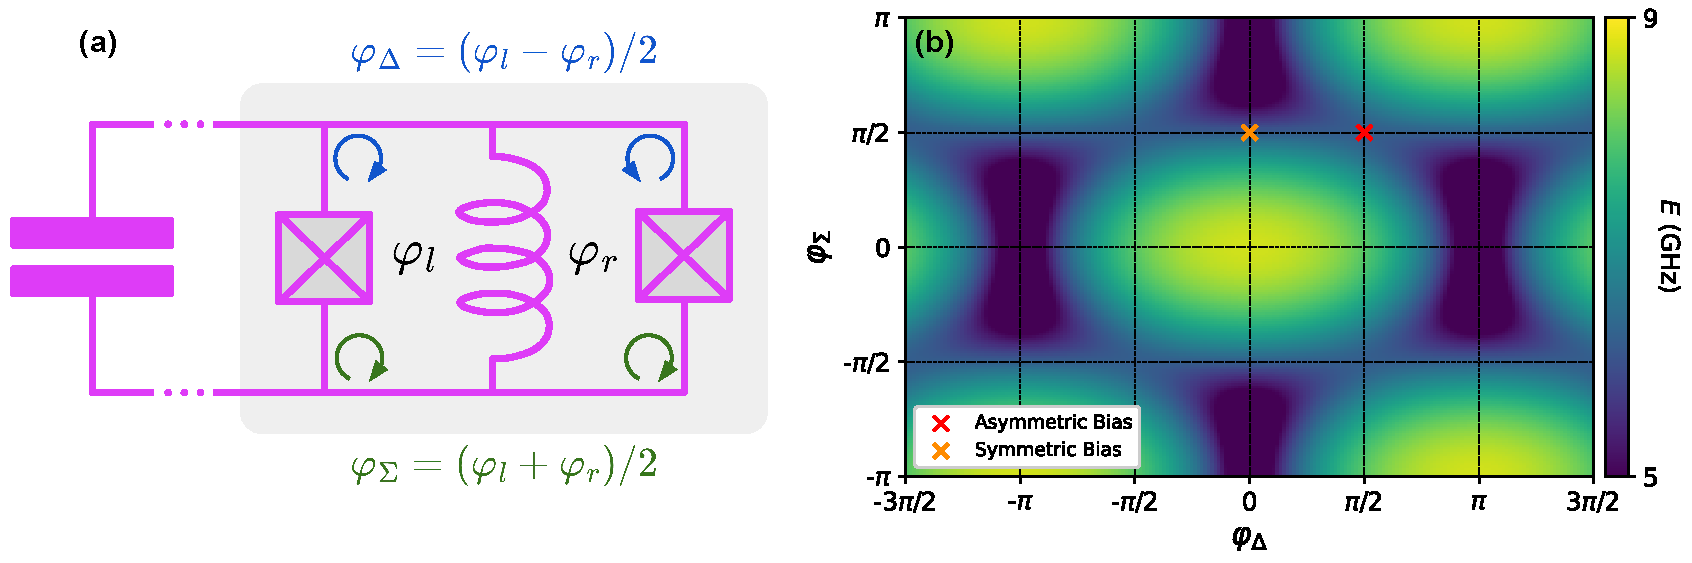
\includegraphics[width=\linewidth]{Figures/5/ats_spectrum.pdf}
    \caption{\textbf{(a)} Circuit diagram for the ATS dipole element (shaded in gray) which consists of a symmetric SQUID shunted by an inductor. The left/right loops are threaded by fluxes $\varphi_l$/$\varphi_r$ respectively, giving rise to common and differential fluxes $\varphi_\Sigma$ and $\varphi_\Delta$. When the ATS is connected to a capacitor, it forms a mode. \textbf{(b)} Fundamental frequency of the ATS mode vs. flux $(\varphi_\Sigma, \varphi_\Delta)$ using parameters $E_L/h = 60$ GHz, $E_J/h = 30$ GHz, and $E_C/h = 80$ MHz.}
    \label{fig:5_ats_spectrum}
\end{figure}

\noindent To begin our exploration of the ATS, let's consider its potential energy, which is given by:
\begin{equation}
    \hat{U}_b = \frac{1}{2}E_L \bigg(\hat{\varphi} + \frac{C_r\varphi_r - C_l\varphi_l}{C_\Sigma}\bigg)^2 - E_{J,l}\cos\!\bigg(\hat{\varphi} + \frac{C_r}{C_\Sigma}[\varphi_l + \varphi_r]\bigg) - E_{J,r}\cos\!\bigg(\hat{\varphi} - \frac{C_l}{C_\Sigma}[\varphi_l + \varphi_r]\bigg)
\end{equation}
Here, we have used the method of Ref. \cite{you2019circuit} to write the potential in terms of its irrotational variable $\hat{\varphi}$, which is the correct approach for time-varying external fluxes; the expression is thus somewhat different from the original description of the ATS in Ref. \cite{lescanne2020exponential}. We have left and right junctions with energies $E_{J, l/r}$, inherent capacitances $C_{l/r}$, and external fluxes $\varphi_{l/r}$ respectively. At this point, we can define the effective $E_J = (E_{J,l} + E_{J,r})/2$ and asymmetry $\Delta E_J = (E_{J,l} - E_{J,r})/2$, and transform to sum and difference coordinates $\varphi_{\Sigma/\Delta} = (\varphi_l \pm \varphi_r)/2$.  Ideally, we would like the junctions to be perfectly symmetric; in practice the asymmetry can be minimized to about $1\%$ of $E_J$. While this is important to keep track of, we will here set $\Delta E_J \to 0$ in the rest of the theory that follows. Thus, $E_{J,l} = E_{J,r} = E_J$ and $C_l = C_r = C$, with $C_\Sigma = C_l + C_r$. We can therefore simplify the complicated expression above and write the potential as:
\begin{equation}
\hat{U}_b(\hat{\varphi}) = \frac{1}{2}E_L(\hat{\varphi} - \varphi_\Delta)^2 - 2E_J \cos(\varphi_\Sigma)\cos(\hat{\varphi})
\end{equation}
In what follows, we will typically keep the differential flux $\varphi_\Delta$ constant and only modulate the common flux $\varphi_\Sigma = \varphi_\Sigma(t)$. Therefore, we can perform a gauge transformation to move the now DC flux $\varphi_\Delta$ to the cosine via $\hat{\varphi} \mapsto \hat{\varphi} + \varphi_\Delta$. This finally get us back to the familiar expression
\begin{equation}
\hat{U}_b(\hat{\varphi}) = \frac{1}{2}E_L\hat{\varphi}^2 - 2E_J \cos(\varphi_\Sigma)\cos(\hat{\varphi} + \varphi_\Delta)
\end{equation}
that can be found in Refs. \cite{lescanne2020exponential, berdou2023one}. We will use this throughout the rest of this chapter.

As shown in Fig. \ref{fig:5_ats_spectrum}(b), when the ATS is connected to a capacitance, the resulting mode has a fundamental frequency that is doubly periodic in $\varphi_\Sigma$ and $\varphi_\Delta$, forming an `egg-carton' potential as it is sometimes referred to. There are two typical operating points for the ATS:

\begin{itemize}
    \item \textbf{Asymmetric bias point:} $(\varphi_\Sigma, \varphi_\Delta) = (\pi/2, \pi/2)$, corresponding to $\varphi_l = \pi$ and $\varphi_r = 0$. This is the standard operating point for the ATS. By modulating the sum flux around this bias, i.e. $\varphi_\Sigma(t) = \pi/2 + \epsilon(t)$, we get the following time-dependent potential for the ATS dipole:
    \begin{equation}
        \hat{U}_b(\hat{\varphi}) = \frac{1}{2}E_L \hat{\varphi}^2 - 2E_J \sin[\epsilon(t)]\sin(\hat{\varphi})
    \end{equation}
\item \textbf{Symmetric bias point:} $(\varphi_\Sigma, \varphi_\Delta) = (\pi/2, 0)$, corresponding to $\varphi_l = \varphi_r = \pi/2$. Biasing here gives us:
\begin{equation}
        \hat{U}_b(\hat{\varphi}) = \frac{1}{2}E_L \hat{\varphi}^2 - 2E_J \sin[\epsilon(t)]\cos(\hat{\varphi})
    \end{equation}
\end{itemize}
%%%%%%%%%%%%%%%%%%%%%%%%
\subsection{The Resonator-ATS-Transmon (RAT)}

Our first approach to faster GKP error correction was developed using the ATS as a coupler element between a storage resonator and a transmon control qubit. We name this the RAT. The basic idea relies on black-box quantization (cf. Ch. \ref{ch:3_cQED}) between the three modes $\hat{a}_0$, $\hat{b}_0$, and $\hat{q}_0$ for the resonator, ATS, and transmon respectively. The bare transmon Hamiltonian is:
\begin{equation}
\hat{H}_{q, 0} = 4E_{C,q}\hat{n}_q^2 - E_{J,q}\cos(\hat{\theta}) = \omega_{q,0}\,\hat{q}_0^\dagger \hat{q}_0 - \Big[E_{J,q}\cos(\hat{\theta}) + \frac{1}{2}E_{J,q} \hat{\theta}^2\Big] 
\end{equation}
where we write the mode $\hat{q}_0$ in terms of the transmon charge $\hat{n}_q$ and phase-drop $\hat{\theta}$. For the ATS, it is:
\begin{equation}
\hat{H}_{b,0} = 4E_C \hat{n}^2 + \hat{U}_b(\hat{\varphi}) = \omega_{b,0}\hat{b}_0^\dagger \hat{b}_0 - 2E_J \cos(\varphi_\Sigma)\cos(\hat{\varphi} + \varphi_\Delta)
\end{equation}
in terms of the ATS charge operator $\hat{n}$ and phase-drop $\hat{\varphi}$. Finally, for the storage we have $\hat{H}_{a, 0} = \omega_{a,0}\hat{a}_0^\dagger \hat{a}_0$. If we take the modes to be linearly coupled (e.g. via capacitive coupling) in series, i.e. resonator $\leftrightarrow$ ATS $\leftrightarrow$ transmon, then the total Hamiltonian has a \textit{linear} part:
\begin{equation}
\hat{H}_{\rm lin, 0} = \omega_{a,0}\hat{a}_0^\dagger \hat{a}_0 + \omega_{b,0}\hat{b}_0^\dagger \hat{b}_0 + \omega_{q,0}\hat{q}_0^\dagger \hat{q}_0 - g_{ab}(\hat{a}_0 - \hat{a}_0^\dagger)(\hat{b}_0 - \hat{b}_0^\dagger) - g_{qb}(\hat{b}_0 - \hat{b}_0^\dagger)(\hat{q}_0 - \hat{q}_0^\dagger)
\end{equation}
Following black-box quantization, we can diagonalize $\hat{H}_{\rm lin, 0}$ as a system of normal modes $\hat{a}$ (storage-like), $\hat{b}$ (buffer-like), and $\hat{q}$ (qubit-like). In this basis $\hat{H}_{\rm lin} = \omega_a \hat{a}^\dagger\hat{a} + \omega_b \hat{b}^\dagger\hat{b} + \omega_q \hat{q}^\dagger\hat{q}$, where $\omega_a$, $\omega_b$, and $\omega_q$ are the normal mode frequencies. We can also rewrite the bare modes in this normal mode basis via a linear transformation:
\begin{align}
\hat{\theta} &= \theta_{q, 0}(\hat{q}_0 + \hat{q}_0^\dagger) = \theta_q(\hat{q} + \hat{q}^\dagger) + \theta_b(\hat{b} + \hat{b}^\dagger) + \theta_a(\hat{a} + \hat{a}^\dagger) \\
\hat{\varphi} &= \phi_{b, 0}(\hat{b}_0 + \hat{b}_0^\dagger) = \phi_q(\hat{q} + \hat{q}^\dagger) + \phi_b(\hat{b} + \hat{b}^\dagger) + \phi_a(\hat{a} + \hat{a}^\dagger)
\label{eq:linear_basis_RAT_RAF}
\end{align}
Here, $\theta_i$ denotes the participation of mode $i$ in the phase across the Josephson junction in the transmon, while $\phi_i$ is the participation in the phase across the ATS. In total, we have
\begin{equation}
\hat{H} = \sum_{c = \{a, b, q\}}\omega_c \hat{c}^\dagger\hat{c} - \Big[E_{J,q}\cos(\hat{\theta}) + \frac{1}{2}E_{J,q} \hat{\theta}^2\Big] - 2E_J \cos(\varphi_\Sigma)\cos(\hat{\varphi} + \varphi_\Delta)
\end{equation}
as the Hamiltonian for the full resonator-ATS-transmon system written in the ``black-box quantization'' basis (i.e. of the normal modes of the linearized circuit). 

With the Hamiltonian written down, let's now see how to get conditional displacements out of it. We park the ATS at its standard asymmetric bias point $(\varphi_\Sigma, \varphi_\Delta) = (\pi/2, \pi/2)$ and modulate $\varphi_\Sigma(t) = \pi/2 + \epsilon(t)$ about this. The ATS potential takes on the form $\sin[\epsilon(t)]\sin(\hat{\varphi})$, and so we can Taylor expand $\sin[\epsilon(t)] \approx \epsilon(t)$ and $\sin(\hat{\varphi}) \approx \hat{\varphi} - \hat{\varphi}^3/6$ in anticipation of making a rotating-wave approximation. We can also truncate the transmon potential to a Duffing oscillator, considering only the leading fourth-order nonlinearity. These approximations give us
\begin{equation}
\hat{H} = \sum_{c = \{a, b, q\}}\omega_c \hat{c}^\dagger\hat{c} - \frac{E_{J,q}}{24}\hat{\theta}^4 - 2E_J \epsilon(t)\hat{\varphi} + \frac{1}{3}E_J\epsilon(t)\hat{\varphi}^3
\end{equation}
We go into a rotating frame for each of the modes $\hat{c} \mapsto \hat{c} e^{-i\tilde{\omega}_c t}$ where we set the frequency $\widetilde{\omega}_c = \omega_c - \theta_{c}^{2} \big[\theta_{a}^{2} + \theta_{b}^{2} + \theta_{q}^{2}\big]/2$ to cancel out the frequency normalizations that arise from the transmon nonlinearity. In this frame, we get
\begin{align}
\begin{split}
\hat{H} &= \hat{H}_{cc} - \frac{E_{J,q}}{24}\Big[\theta_q(\hat{q}e^{-i\tilde{\omega}_q t} + \hat{q}^\dagger e^{i\tilde{\omega}_q t}) + \theta_b(\hat{b}e^{-i\tilde{\omega}_b t} + \hat{b}^\dagger e^{i\tilde{\omega}_b t}) + \theta_a(\hat{a}e^{-i\tilde{\omega}_a t} + \hat{a}^\dagger e^{i\tilde{\omega}_a t})\Big]^4 \\&\quad- 2E_J\epsilon(t)\Big[\phi_q(\hat{q}e^{-i\tilde{\omega}_q t} + \hat{q}^\dagger e^{i\tilde{\omega}_q t}) + \phi_b(\hat{b}e^{-i\tilde{\omega}_b t} + \hat{b}^\dagger e^{i\tilde{\omega}_b t}) + \phi_a(\hat{a}e^{-i\tilde{\omega}_a t} + \hat{a}^\dagger e^{i\tilde{\omega}_a t})\Big]\\ &\quad + \frac{1}{3}E_J\epsilon(t)\Big[\phi_q(\hat{q}e^{-i\tilde{\omega}_q t} + \hat{q}^\dagger e^{i\tilde{\omega}_q t}) + \phi_b(\hat{b}e^{-i\tilde{\omega}_b t} + \hat{b}^\dagger e^{i\tilde{\omega}_b t}) + \phi_a(\hat{a}e^{-i\tilde{\omega}_a t} + \hat{a}^\dagger e^{i\tilde{\omega}_a t})\Big]^3
\end{split}
\end{align}
where $\hat{H}_{cc} = \sum (\omega_c - \tilde{\omega}_c)\hat{c}^\dagger\hat{c}$ will cancel out when the terms are expanded. At this point our task involves sorting through the various pumped nonlinear terms and keeping only the ones that survive the RWA. We set $\epsilon(t) = \epsilon_p \sin(\omega_p t)$ with $\omega_p = \tilde{\omega}_a$, picking out terms that rotate at the (renormalized) storage frequency. Luckily we can do the oscillator expansion, normal ordering, and RWA all numerically using SymPy. The final effective Hamiltonian
\begin{align}
\begin{split}
\hat{H}_{\rm eff} &= \frac{K_a}{2}{{a}^\dagger}^{2} {a}^{2} + \frac{K_b}{2}{{b}^\dagger}^{2} {b}^{2} + \frac{K_q}{2}{{q}^\dagger}^{2} {q}^{2} + \frac{\chi_{ab}}{2}\hat{a}^\dagger\hat{a}\hat{b}^\dagger\hat{b} + \frac{\chi_{aq}}{2} \hat{a}^\dagger\hat{a}\hat{q}^\dagger\hat{q} + \frac{\chi_{qb}}{2} \hat{q}^\dagger\hat{q}\hat{b}^\dagger\hat{b} \\
&\quad + g_{\rm CD}{{q}^\dagger} {q}\big(\hat{a} + \hat{a}^\dagger\big) + g_{\rm disp} \big(\hat{a}+\hat{a}^\dagger\big) + g_a\big[{{a}^\dagger} {a}^{2} + {{a}^\dagger}^{2} {a}\big] + g_b {{b}^\dagger} {b}\big(\hat{a} + \hat{a}^\dagger\big) 
\end{split}
\end{align}
has many terms that we can categorize as follows. We have Kerr nonlinearities for all three modes $K_x = -E_{J, q}\theta_{x}^{4} / 2$ and cross-Kerr dispersive shifts $\chi_{xy} = -2E_{J, q}\theta_{x}^{2} \theta_{y}^{2}$. Next, we have the desired conditional displacement $g_{\rm CD} = E_J\epsilon_{p} \phi_{a} \phi_{q}^{2}$ and an unconditional displacement $g_{\rm disp} = E_J\epsilon_p\big[\phi_a^3 +\phi_{a} \phi_{q}^{2} + \phi_{a} \phi_{b}^{2} - 2\phi_a\big]/2$. Finally, we also have two spurious nonlinear terms associated with the storage and ATS mode: $g_a = E_J\epsilon_{p} \phi_{a}^{3}/2$ and $g_b = E_J\epsilon_{p} \phi_{a}\phi_{b}^{2}$. The qubit anharmonicity $K_q$ should not affect the oscillator dynamics, and just provides the requisite nonlinearity for control. Furthermore, if the ATS is never strongly populated $\ev{\hat{b}^\dagger\hat{b}} \approx 0$, we can further simplify to just:
\begin{equation}
\hat{H}_{\rm eff} = \frac{\chi_{aq}}{2} \hat{a}^\dagger\hat{a}\hat{q}^\dagger\hat{q} + \frac{K_a}{2}{{a}^\dagger}^{2} {a}^{2} + g_{\rm CD}{{q}^\dagger} {q}\big(\hat{a} + \hat{a}^\dagger\big) + g_{\rm disp} \big(\hat{a}+\hat{a}^\dagger\big) + g_a\big[{{a}^\dagger} {a}^{2} + {{a}^\dagger}^{2} {a}\big]
\label{eq:5_FCD_full_hamiltonian}
\end{equation}
Overall, we have the desired conditional displacement term, along with several additional unwanted terms that we will now discuss how to cancel out. Note that all drive-activated terms are proportional to the flux pump envelope $\epsilon_p = \epsilon_p(t)$, which we can pulse to activate the desired interactions. 

\subsection{Conditional Displacements with the RAT}

It turns out that we can cancel many of the unwanted terms above using an echo protocol reminiscent of the echoed conditional displacement (ECD) from Ref. \cite{eickbusch2022fast} that we reviewed in Ch. \ref{ch:2_QEC}. To see how, let's consider a simplified version of Eq. \eqref{eq:5_FCD_full_hamiltonian} with just the CD term and the dispersive shift. We also truncate the transmon to a two-level qubit $\hat{q}^\dagger\hat{q} \to \hat{\sigma}_z$ and thus have:
\begin{equation}
\hat{H}(t) = \frac{\chi}{2}\hat{a}^\dagger\hat{a}[z(t)\hat{\sigma}_z]   + \Big[g_{\rm CD}(t)\hat{a}^\dagger + g_{\rm CD}^\ast(t)\hat{a}\Big]z(t)\hat{\sigma}_z
\label{eq:5_FCD_simplified_hamiltonian}
\end{equation}
Here we have included a fictitious qubit state parameter $z(t) = \ev{\sigma_z(t)}$ that tells us when to perform $\pi$-pulses \cite{eickbusch2022fast}, and also explicitly highlight the time-dependence $g_{\rm CD}(t)$ controlled via the flux pump. We can then solve the Schr\"odinger equation $i\partial_t\hat{U} = \hat{H}(t)\hat{U}$ in terms of a parameterized ansatz $\hat{U}(t)$. We find the same ansatz and solution as Ref. \cite{eickbusch2022fast}: 
\begin{equation}
    \hat{U}(t) = \exp(i\theta \hat{\sigma}_z / 2)\,\exp\!\Big[\hat{a}^\dagger(\gamma + \delta \hat{\sigma}_z) - \hat{a}(\gamma^\ast + \delta^\ast \hat{\sigma}_z)\Big]\exp(i\phi\hat{a}^\dagger\hat{a}\hat{\sigma}_z)
\end{equation}
where $\theta(t), \gamma(t), \delta(t), \phi(t)$ correspond to a qubit rotation, cavity displacement and conditional displacement, and a qubit-selective cavity rotation. Plugging in Eq. \eqref{eq:5_FCD_simplified_hamiltonian} and solving the Schr\"odinger equation, it turns out we can actually find a solution:
\begin{align}
    \begin{split}
        \theta(t) & = +2 \int_0^t d\tau \mathrm{Re}[g_{\rm CD}^*(\tau)\gamma(\tau)] \qquad \qquad\delta(t) = -i \int_0^t d\tau \cos[\phi(\tau)-\phi(t)] g_{\rm CD}(\tau)z(\tau) \\\gamma(t) & = - \int_0^t d\tau \sin[\phi(\tau)-\phi(t)] g_{\rm CD}(\tau)z(\tau) \qquad \qquad\phi(t) = -\frac{\chi}{2} \int_0^t d\tau z(\tau)
    \end{split}
\end{align}
If the CD gate has length $T$, we want $\phi(T) = 0$ at the end of the gate, and thus $\int z(\tau)d\tau = 0$, i.e. the area under the curve of $z(t)$ must be net zero. This implies that the qubit state $z(t)$ has to flip signs at least once! Furthermore, as with the ECD protocol, if we consider only $\pi$-pulses on the qubit, then $z \in \{1, -1\}$. These requirements constrain the pulse schedule $z(t)$ to take on the form of a Walsh function \cite{chalermpusitarak2021frame}. To cancel the \textit{unconditional} displacement and keep just a \textit{conditional} displacement, we next want to set
\begin{equation*}
    \gamma(T) = - \int_0^T \!d\tau \sin[\phi(\tau)] g_{\rm CD}(\tau)z(\tau) = 0, \,\,\text{and}\,\, \delta(T) = -i \int_0^T \!d\tau \cos[\phi(\tau)] g_{\rm CD}(\tau)z(\tau) \neq 0.
\end{equation*}
At this point, observe that if $g_{\rm CD}(t)z(t)$ can be made constant over the gate length $T$, then the symmetries of sine and cosine will automatically ensure $\gamma(T) = 0$ and $\delta(T) \neq 0$. Since the $\pi$-pulse schedule $z(t)$ is constained in its form, we can try several ansatze and modulate $g_{\rm CD}(t)$ with the same time-dependence so that $z(t)g_{\rm CD}(t)$ is constant. We find that a double-echo schedule satisfies all of our requirements, with $\pi$-pulses at $t = T/4$ and $t = 3T/4$, and $z(0)=1$ to initialize the qubit in the ground state $\ket{g}$. An example is plotted below, along with the final pulse sequence for $g_{\rm CD}(t)$ [which, again, is set by modulating the flux pump amplitude $\epsilon_p(t)$]. We named this novel sequence the \textbf{f}ast echoed \textbf{c}onditional \textbf{d}isplacement, or FCD, to contrast it from the usual ``single-echo'' ECD that we saw in Ch. \ref{ch:2_QEC}. 

\begin{figure}[t]
    \centering
    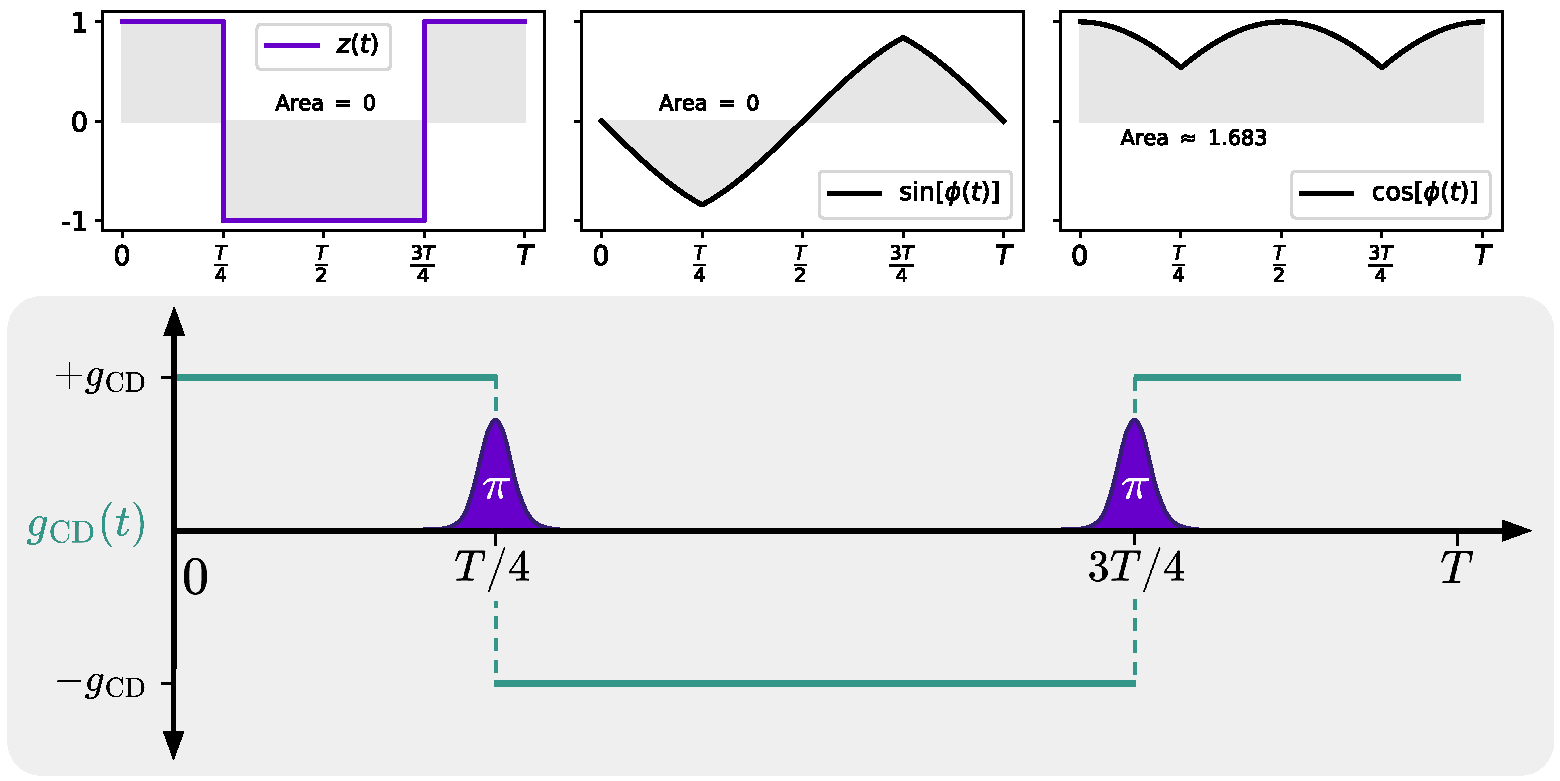
\includegraphics[width=\linewidth]{Figures/5/double_echo_FCD.pdf}
    \caption{FCD pulse implementation using the double-echo $\pi$-pulse schedule $z(t)$. Top row: numerical example of $z(t)$, $\sin[\phi(t)]$, and $\cos[\phi(t)]$ for $T = 2$ and $\chi = 4$. Observe $z(t)$ has an integral of zero as required. By modulating $g_{\rm CD}(t)$ to match the time-dependence of $z(t)$, we get constant $g_{\rm CD}(t)z(t) = 1$. The areas under $\sin[\phi(t)]$ and $\cos[\phi(t)]$ then give the relative magnitudes of the unconditional and conditional displacement rates in the FCD unitary. Bottom row: full ideal FCD pulse sequence showing the $\pi$-pulses and $g_{\rm CD}(t)$.}
    \label{fig:5_double_echo_FCD}
\end{figure}

We performed numerical simulations of the FCD gate using a two-level qubit truncated version of the full Hamiltonian in Eq. \eqref{eq:5_FCD_full_hamiltonian}, and found that the double $\pi$-pulse sequence we constructed indeed allows us to echo away the unwanted terms (such as the dispersive term $\chi_{aq}$, the displacement $g_{\rm disp}$, and the nonlinear displacement $g_a$). Unfortunately, however, we also find that the strength of the unconditional displacement $g_{\rm disp}$ in this scheme can be much larger than the conditional displacement $g_{\rm CD}$; using realistic device parameters we found that $g_{\rm disp}$ is often an order of magnitude larger. As a result, we expect that a separate ``cancellation drive'' on the storage will be required if we want to implement the FCD scheme in practice. 

Beyond this, we also found that the various design constraints for a realistic RAT device can be quite demanding, as it is somewhat difficult to hit the various couplings and mode capacitances during design/simulation. Moreover, the transmon control qubit in the RAT approach would still be susceptible to frequent bit-flip errors, limiting the GKP code performance. For these reasons, we chose to develop an alternative to the RAT with a fluxonium control qubit in place of the transmon; we will discuss this next. 

Despite the challenges associated with it, the RAT remains a novel and interesting theoretical proposal for implementing GKP error correction, and we hope the ideas behind it may be useful in developing further experiments in the future. 
 \clearpage
 %%%%%%%%%%%%%%%%%%%%%%%%

\section{The Resonator-ATS-Fluxonium (RAF) Experiment \label{sec:5_RAF}}

Our current main approach to realizing GKP error correction in 2D is called the RAF. It builds upon the idea of using an ATS as a coupler to realize fast conditional displacements, but instead uses a heavy fluxonium control qubit. To understand the principle behind the RAF, we start from the Hamiltonian for a coupled a storage resonator, ATS, and fluxonium system: $\hat{H} = \hat{H}_a + \hat{H}_b + \hat{H}_q + \hat{H}_{\rm int}$, where $\hat{H}_{\rm int}$ is a linear capacitive coupling term and $\hat{H}_q$ is:
\begin{equation}
    \hat{H}_q = 4E_C \hat{n}_q^2 + \frac{1}{2}\hat{\theta}^2 - E_J\cos(\hat{\theta}-\theta{\rm ext}) = \omega_{q, 0} \hat{q}_0^\dagger\hat{q}_0 - E_J\cos(\hat{\theta}-\theta{\rm ext})
\end{equation}
Here we have written the fluxonium Hamiltonian in its ``LC basis'' (i.e. the Fock basis for the linear part of the circuit). Following our approach in Sec. \ref{sec:5_RAT}, we can now analyze the full coupled system using a normal mode basis, i.e. absorbing the linear coupling term to get three normal modes $\hat{a}$, $\hat{b}$, and $\hat{q}$ for the storage, ATS, and qubit respectively. In this basis, 
\begin{equation}
    \hat{H} = \sum_{c = \{a, b, q\}}\omega_c \hat{c}^\dagger \hat{c} - E_{J,q}\cos(\hat{\theta}-\theta_\mathrm{ext}) - 2E_J \cos(\varphi_\Sigma)\cos(\hat{\varphi} + \varphi_\Delta)
    \label{eq:RAF_H}
\end{equation}
where the phase operators $\hat{\theta}$ and $\hat{\varphi}$ for the fluxonium and ATS may be expressed as linear combinations of $\hat{a}, \hat{a}^\dagger$, $\hat{b}, \hat{b}^\dagger$, and $\hat{q}, \hat{q}^\dagger$ as in Eq. \eqref{eq:linear_basis_RAT_RAF}, in terms of the participations $\theta_a, \theta_b, \theta_q$ ($\phi_a, \phi_b, \phi_q$) of the the various modes in the fluxonium (ATS) phase. This basis is reminiscent of black-box quantization, but we stress here that no approximation has been made --- as long as we do not truncate the fluxonium, Eq. \eqref{eq:RAF_H} is exact. 

To implement conditional displacements with the RAF, we bias the ATS at the \textit{symmetric} bias point $(\varphi_\Sigma, \varphi_\Delta) = (\pi/2, 0)$ and modulate about this via $\varphi_\Sigma(t) = \pi/2 + \epsilon(t)$. In this case, we get
\begin{equation}
    \hat{H} = \sum_{c = \{a, b, q\}}\omega_c \hat{c}^\dagger \hat{c} - E_{J,q}\cos(\hat{\theta}-\theta_\mathrm{ext}) - 2E_J \sin[\epsilon(t)]\cos\hat{\varphi}
    \label{eq:RAF_H_biaspoint}
\end{equation}
The fluxonium nonlinear term will now give rise to dispersive shifts $\chi_{xy}$ between the three modes, as well as Kerr nonlinearities $K_x$ for $x, y \in \{a, b, q\}$, while the ATS nonlinear term will give us the desired microwave-activated conditional displacement interaction. Let's now focus on the latter term. We can write $\hat{\varphi} = \hat{\varphi}_a + \hat{\varphi}_b + \hat{\varphi}_q$ and Taylor expand the drive $\sin[\epsilon(t)] \approx \epsilon(t) = \epsilon_p\cos(\omega_p t)$. Doing so, we can express this part of the Hamiltonian $\hat{H}_{\rm CD}$ as follows:
\begin{equation}
    \hat{H}_{\rm CD} = - 2E_J\epsilon(t)\big[\cos\hat{\varphi}_q\cos{(\hat{\varphi}_a + \hat{\varphi}_b)} - \sin\hat{\varphi}_q\sin{(\hat{\varphi}_a + \hat{\varphi}_b)}\big]
    \label{eq:RAF_HCD_expanded}
\end{equation}
Here, we have used a trigonometric identity to separate out the qubit ($\hat{\varphi}_q$) terms from the others, for the following reason. The storage $\hat{\varphi}_a = \varphi_a(\hat{a} + \hat{a}^\dagger)$ and ATS $\hat{\varphi}_b= \varphi_b(\hat{b} + \hat{b}^\dagger)$ both have small phase fluctuations, which will allow us to Taylor expand using $\varphi_a, \varphi_b$ as small parameters. Meanwhile, the fluxonium \textit{cannot} be expanded in this manner, and thus we must keep the full nonlinearities $\sin(\hat{\varphi}_q)$ and $\cos(\hat{\varphi}_q)$. Keeping this in mind, we can expand to 
\begin{equation*}
    \cos{(\hat{\varphi}_a + \hat{\varphi}_b)} = \cos\hat{\varphi}_a\cos \hat{\varphi}_b - \sin\hat{\varphi}_a\sin \hat{\varphi}_b \approx \bigg[1 - \frac{\hat{\varphi}_a^2}{2}\bigg]\bigg[1 - \frac{\hat{\varphi}_b^2}{2}\bigg] - \hat{\varphi}_a\hat{\varphi}_b
\end{equation*}
and 
\begin{equation*}
    \sin{(\hat{\varphi}_a + \hat{\varphi}_b)} = \sin\hat{\varphi}_a\cos \hat{\varphi}_b + \cos\hat{\varphi}_a\sin \hat{\varphi}_b \approx \hat{\varphi}_a\bigg[1 - \frac{\hat{\varphi}_b^2}{2}\bigg] + \hat{\varphi}_b\bigg[1 - \frac{\hat{\varphi}_a^2}{2}\bigg]
\end{equation*}
If we now go into the rotating frames of modes $a$ and $b$, and further set the ATS flux drive frequency to the storage frequency $\omega_p = \omega_a$, then we can perform an RWA on Eq. \eqref{eq:RAF_HCD_expanded} to get an effective
\begin{equation}
    \hat{H}_{\rm CD} = 2E_J \bigg[1 - \frac{\varphi_b^2}{2} - \varphi_b^2\hat{b}^\dagger\hat{b}\bigg]\bigg(\frac{\epsilon_p}{2}\bigg)\hat{\varphi_a}\sin(\hat{\varphi}_q)
\end{equation}
Finally, assuming that the ATS mode is never populated due to its detuning from the other modes, we set $\ev{\hat{b}^\dagger\hat{b}} \approx 0$ and can then expand $\hat{\varphi}_a = \varphi_a(\hat{a} + \hat{a}^\dagger)$ to get a final effective Hamiltonian
\begin{equation}
    \hat{H}_{\rm CD} = E_J  \epsilon_p\varphi_a \bigg[1 - \frac{\varphi_b^2}{2} \bigg](\hat{a} + \hat{a}^\dagger)\sin\hat{\varphi}_q \triangleq \hat{H}_{\rm CD}^{(q)} (\hat{a} + \hat{a}^\dagger)
\end{equation}
where we group the prefactors and qubit terms into $\hat{H}_{\rm CD}^{(q)}$. From here, we can calculate the displacement and conditional displacement rates via the sum and difference matrix elements of the qubit part:
\begin{align}
    \begin{split}
        g_\mathrm{disp} &= \frac{1}{2}\Big[\langle g|\hat{H}_{\rm CD}^{(q)}|g\rangle + \langle e|\hat{H}_{\rm CD}^{(q)}|e\rangle \Big] = A\bigg[\langle g|\sin\hat{\varphi}_q|g\rangle + \langle e|\sin\hat{\varphi}_q|e\rangle\bigg] \\
        g_{\rm CD} &= \frac{1}{2}\Big[\langle g|\hat{H}_{\rm CD}^{(q)}|g\rangle - \langle e|\hat{H}_{\rm CD}^{(q)}|e\rangle \Big] = A\bigg[\langle g|\sin\hat{\varphi}_q|g\rangle - \langle e|\sin\hat{\varphi}_q|e\rangle\bigg]
    \end{split}
\end{align}
with a common scale factor $A = \frac{1}{2}E_J\epsilon_p   \varphi_a[1 - \varphi_b^2/2]$. If we truncate the qubit to a two-level subspace, we get
\begin{equation}
    \hat{H}_{\rm CD}^{\rm tls} = g_{\rm disp} (\hat{a}+\hat{a}^\dagger) + g_{\rm CD} (\hat{a}+\hat{a}^\dagger)\hat{\sigma}_z
\end{equation}
This is precisely the conditional displacement interaction we wanted, though it also comes with an additional direct displacement. It so happens, however, that for a heavy-fluxonium away from half-flux, the difference in matrix elements (i.e. $g_{\rm CD}$) can be quite large, while the sum (i.e. $g_{\rm disp}$) can be made quite small; nonetheless, we envision using a cancellation drive to null out the displacement. 

In practice, starting from Eq. \eqref{eq:RAF_H_biaspoint}, we diagonalize the qubit Hamiltonian numerically to compute \textit{all} metrics of interest, such as dispersive shifts and Kerr nonlinearities, in terms of the relevant fluxonium matrix elements. Going from this theoretical proposal to a fully realized experiment took many rounds of design, simulation, and refinement of the theory before we arrived at a final parameter set for the system that satisfied all of the experimental design constraints. I will not discuss these details here; for a more complete treatment, I direct readers to the SM thesis of my colleague Shantanu Jha. 

Instead, I will here just briefly summarize the main results. For our final choice of system parameters, we are able to achieve a large conditional displacement rate $g_{\rm CD}/2\pi \simeq 4$ MHz over a wide range of qubit external flux bias points as shown in Fig. \ref{fig:5_RAF_Metrics}. Over this range, the dispersive shift $\chi_{aq}$ between the fluxonium and storage remains small, and so we don't expect to be limited by oscillator dephasing during qubit reset (which, as we recall from Ch. \ref{ch:4_3DGKP}, was an important consideration in our 3D dispersive experiment and the reason we engineered a flux-tunable dispersive shift to cross through zero there). Lastly, the Kerr nonlinearities $K_g$ and $K_e$ inherited by the storage resonator are neglible (mHz-level). With these values, we expect to be able to achieve state-of-the-art GKP QEC performance. In Fig. \ref{fig:5_RAF_Final_Design}, I also show a false-color image of the final design for the RAF, which is being fabricated as of this writing. In addition the core storage, ATS, and fluxonium subsystem, we have also incorporated a readout resonator and Purcell filter to be able to achieve faster unconditional qubit reset in approximately 100 ns via fluxonium sideband cooling. With this, we expect to be able to perform a cycle of SBS error correction within $\delta t = 400$ ns. 

\begin{figure}[h]
    \centering
    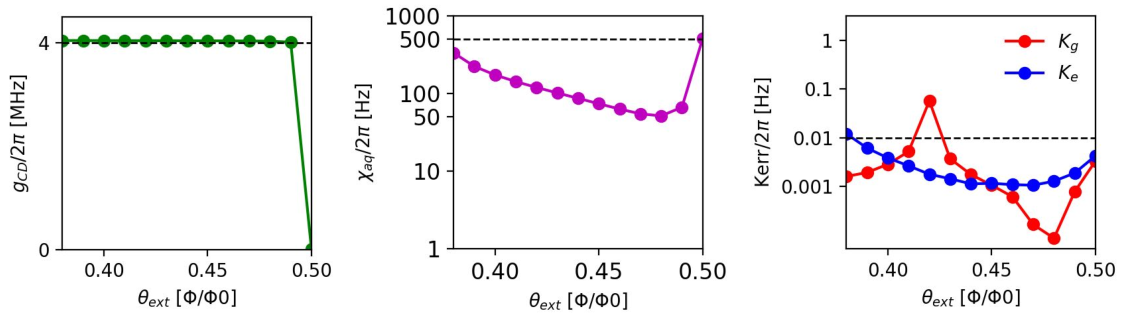
\includegraphics[width=0.95\linewidth]{Figures/5/RAF_Metrics.pdf}
    \caption{Simulated metrics of interest for the RAF using our final design parameters. We get a CD rate of $g_{\rm CD}/2\pi \simeq 4$ MHz across a wide band of external flux operating points $\theta_{\rm ext}$ for the qubit, as well as low residual dispersive shift $\chi_{aq}$ to the storage ($< 0.5$ kHz) and negligible (mHz-level) Kerr nonlinearity.}
    \label{fig:5_RAF_Metrics}
\end{figure}

\begin{figure}[h]
    \centering
    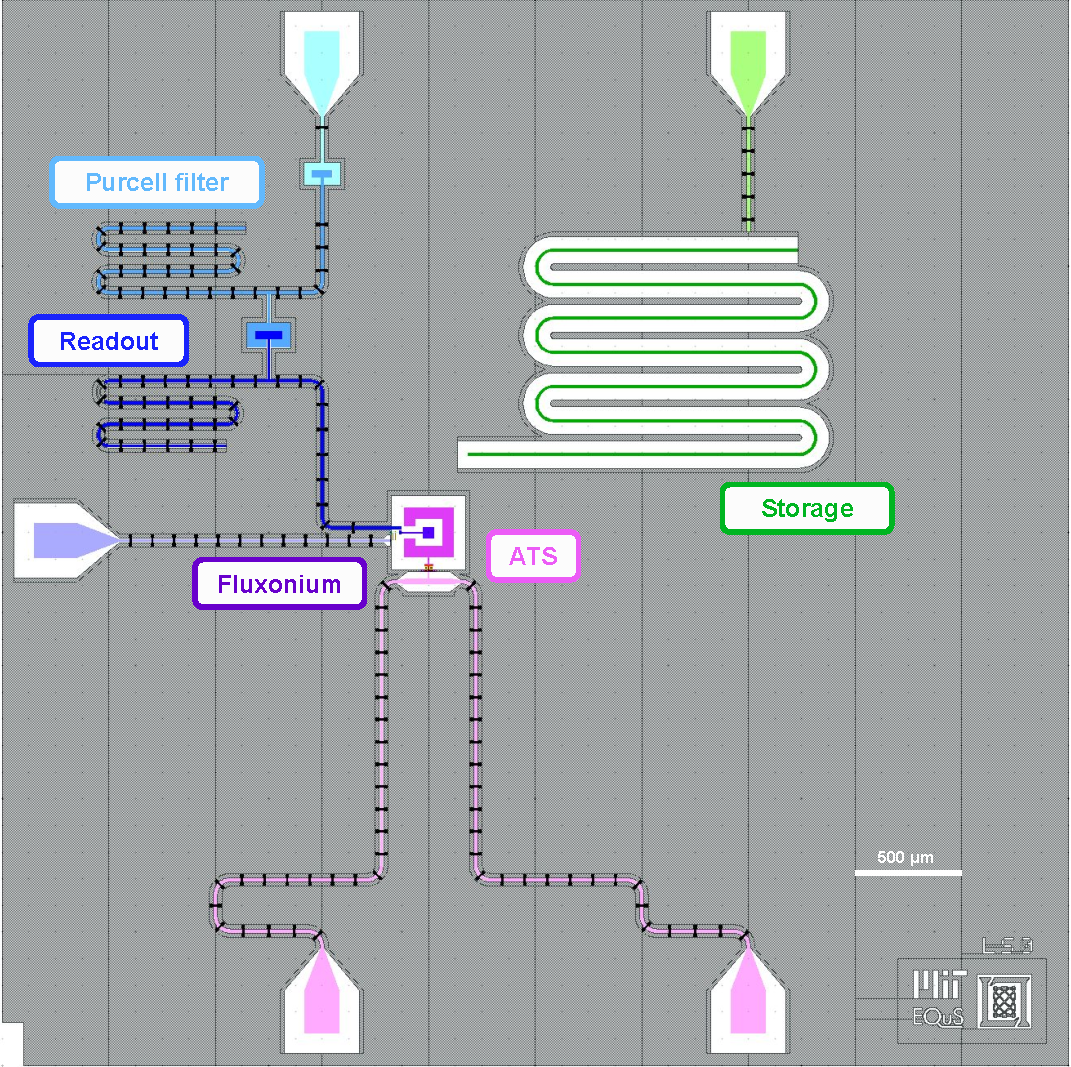
\includegraphics[width=0.7\linewidth]{Figures/5/RAF_Final_Design.pdf}
    \caption{Final chip design for the RAF, consisting of a storage resonator, ATS coupler, and fluxonium control qubit, as well as a readout resonator and Purcell filter for fast reset. For more details, we invite readers to refer to the upcoming SM thesis of Shantanu Jha.}
    \label{fig:5_RAF_Final_Design}
\end{figure}

\clearpage


\section{The 2D Dispersive Experiment: Moving 3D \texorpdfstring{$\to$}{to} 2D\label{sec:5_2D_Disp}}

Our final proposed approach to implement GKP error correction in 2D is our so-called 2D dispersive project. We came up with this approach during the penultimate stage of design for the RAF, which also coincided with our last attempts to fix the storage coherence issues in our 3D dispersive experiment (these issues turned out to be inherent to our 3D package). Given the daunting possibility of having to redesign the 3D experiment from scratch this late into the project, we set out to identify as many alternative paths forward as possible and ultimately settled on the following: why not move the dispersive coupling experiment entirely to 2D, replacing the 3D cavity with an on-chip resonator? This idea was attractive to us for several key reasons: 
\begin{enumerate}
    \item In 2D, the storage and fluxonium can be directly coupled capacitively and we don't need an antenna to mediate the coupling. By reducing one linear mode, this would help alleviate the parasitic Purcell resonances that we saw in  Sec. \ref{sec:4_fluxonium_T1}.
    \item In contrast to 3D, fast-flux control of the qubit can be implemented straightforwardly via on-chip flux lines in 2D. 
    \item Specific to our fabrication workflow in EQuS, a 2D design could be fabricated using a standard 2" wafer at Lincoln Lab as opposed to the 8" wafer that was required for the fluxonium chips we used in our 3D experiment; using the more standard process would help with fabrication time, yield, and parameter targeting. 
    \item We could use the design/simulation infrastructure already developed for the RAF to expedite the process. Indeed, this ultimately proved to be the single most important factor and enabled us to go from ideation to a complete design in under two months. 
    \item It is a simpler 2D experiment than the RAF, and so helps mitigate the risk of failure. 
\end{enumerate}

Of course, as we noted in the previous section, 2D resonators have higher single-photon losses. A 2D dispersive design relying on ECD would not be able to correct such errors as efficiently as the RAF. Nonetheless, given our strategy of using a large gap low-frequency resonator, it seems within the realm of possibility to achieve a storage resonator lifetime of $T_1 \simeq 100$ $\mu$s. As we will see below, this would already be enough to demonstrate QEC. 

\subsection{System Parameters and Design Overview}
The 2D dispersive design consists of four main elements: the storage resonator, fluxonium qubit, readout resonator, and a Purcell filter to help achieve larger resonator linewidth for the SBS reset without causing excess loss to the qubit. As with the RAF, the various design parameters here were chosen to balance many different experimental constraints, and had to be iteratively refined via successive rounds of simulation. The final design is shown in Fig. 5-1, and we will now discuss some of the design considerations that went into it.
\begin{figure}[h] 
    \begin{subfigure}{\linewidth}
        \centering
        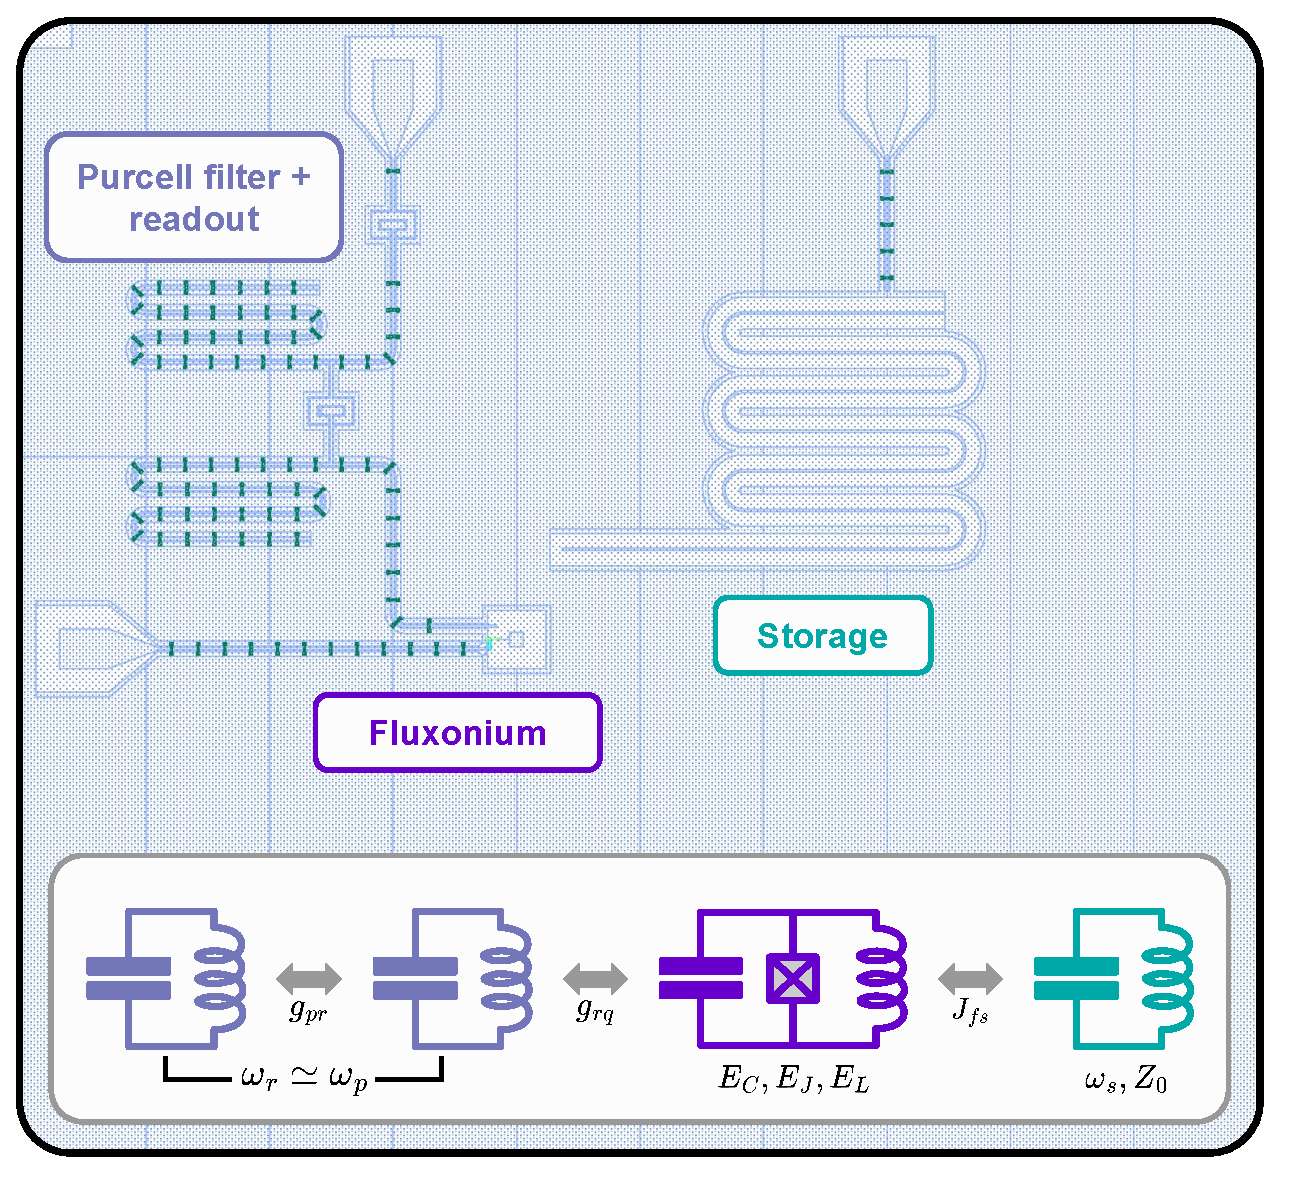
\includegraphics[width=0.8\linewidth]{Figures/5/2D_Dispersive_GDS.pdf}
        \vspace*{2mm}
    \end{subfigure} 
    \begin{subfigure}{\linewidth}
        \centering
        \begin{tabular}{c|c|c|c|c|c|c|c|c }
       $\omega_s/2\pi$ & $J_{fs}/2\pi$ & $E_J/h$  & $E_C/h$ & $E_L/h$ & $g_{rq}/2\pi$ & $\omega_r/2\pi$ & $\omega_p/2\pi$ & $g_{pr}/2\pi$\\\hline
        4134.0 & 3.0 & 3754.9 & 844.0 & 299.9 & 42.1 & 6125.0 & 6137.0 & 27.6
    \end{tabular}
    \end{subfigure}
    \caption{Final GDS design and parameters for the 2D dispersive experiment, showing the on-chip storage resonator, fluxonium qubit, readout resonator, and Purcell filter. The frequency parameters for the various elements in the table are all listed in MHz}
    \label{fig:5_2D_Dispersive_GDS}
\end{figure}

\noindent \textbf{Fluxonium:} We chose the nominal qubit parameters $E_J, E_C, E_L$ shown above in Fig. \ref{fig:5_2D_Dispersive_GDS} to achieve a moderately heavy fluxonium with a frequency of $\omega_q/2\pi \simeq 107$ MHz at half-flux. We expect this will result in a long $T_1^{g\to e}$ away from the sweet spot. These parameters also ensured that the qubit plasmon transition frequencies were high enough to not be limited by heating out of the $\ket{g}$-$\ket{e}$ manifold. 


\noindent \textbf{Storage and Fluxonium System:} The storage mode was designed as a large gap (60 $\mu$m) $\lambda/4$ coplanar waveguide resonator with a resulting impedance of $Z_0 = 95.127$ $\Omega$. We chose its frequency to be as low as possible to maximize $T_1$ given a constant $Q = \omega_s T_1$, ultimately settling on $\omega_s/2\pi = 4.134$ GHz. This was co-designed with the fluxonium so as to achieve bosonic mode threading. For the fluxonium-storage coupling $J_{fs}$, we performed numerical diagonalization simulations of the following Hamiltonian (similar to that in Ch. \ref{sec:4_3D_Experiment_Design_Theory}):
\begin{equation}
    \hat{H} =  \hat{H}_s + \hat{H}_{\rm int} + \hat{H}_{\rm fluxonium} =  \omega_s \hat{a}^\dagger \hat{a} + J_{fs} \hat{n}\hat{n}_a + \Big[4E_C \hat{n}^2 + \frac{1}{2}\hat{\varphi}^2 - E_J\cos(\hat{\varphi}-\varphi_{\rm ext})\Big],
\end{equation}
using which we calculated the dispersive shift $\chi = \omega_s^{|e\rangle} - \omega_s^{|g\rangle} = [E_{e,1} - E_{e, 0}] - [E_{g, 1} - E_{g, 0}]$ as well as the storage Kerr nonlinearities $K = (K_g + K_e)/2$ and $dK = (K_g - K_e)/2$ defined by $K_{g/e} = E_{g/e, 2} + E_{g/e, 0} - 2E_{g/e, 1}$. We then manually varied $\omega_s$ and $J_{fs}$ so as to achieve a low $K$ and $dK$ (on the order of Hz)\footnote{We have seen in simulations that the average Kerr $K$ is worse for GKP performance than differential Kerr $dK$. We can typically afford $dK$ to be slightly (as much as 5-10x) larger than $K$; ideally we have $K < 5$ Hz.} over the external flux range of interest $\Phi_{\rm ext}/\Phi_0 \in [0.42, 0.5]$, while also having a flux-tunable $\chi$ that crosses through zero and that is large enough away from this zero-crossing to perform ECD. We tried to target similar values for $\chi$, $K$, and $dK$ as Ref. \cite{sivak2023gkp-expt}, and ultimately chose the operating point $\Phi_{\rm ext} \simeq 0.43\Phi_0$ where $\chi/2\pi \simeq 50$ kHz, $K/2\pi \simeq 1$ Hz, and $dK/2\pi \simeq 10$ Hz, as shown in Fig. \ref{fig:5_2D_dispersive_metrics}(c). Meanwhile, the reset point at which the storage dispersive shift $\chi \to 0$ occurs at $\Phi_{\rm ext} \simeq 0.475\Phi_0$. 
\begin{figure}[h]
    \centering
    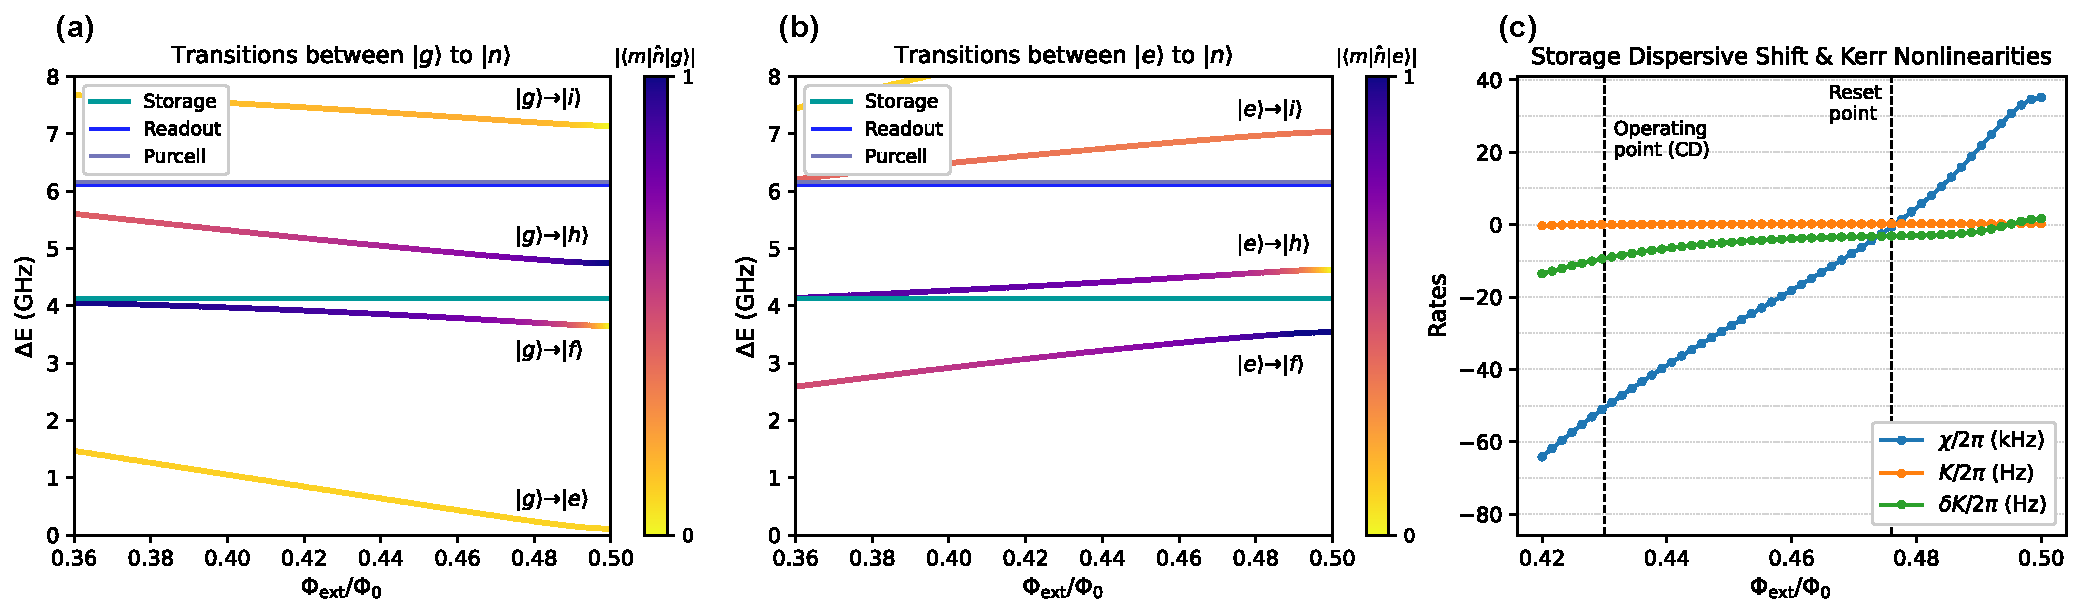
\includegraphics[width=\linewidth]{Figures/5/2D_dispersive_metrics.pdf}
    \caption{\textbf{(a, b)} Simulated fluxonium spectrum for 2D dispersive experiment showing transitions $\ket{g/e}\to\ket{n}$ and the associated charge matrix elements. The storage mode (teal) is threaded between the two sets of plasmon transitions. \textbf{(c)} Simulated storage dispersive shift $\chi$ (kHz), average Kerr $K$ (Hz) and differential Kerr $dK$ (Hz). We label the operating points where we perform reset and conditional displacements (CD) respectively.}
    \label{fig:5_2D_dispersive_metrics}
\end{figure}

\noindent \textbf{Readout and Purcell Filter:} We used a similar design for the readout resonator and Purcell filter as the RAF; both resonators were standard 50 $\Omega$ coplanar waveguide resonators with frequencies $\omega_r/2\pi = 6.125$ and $\omega_p/2\pi = 6.137$. We chose $g_{pr}$ to be greater than the detuning of the modes, so that the two are almost fully hybridized with normal mode frequencies of roughly $\omega_r - g_{pr}$ and $\omega_p + g_{pr}$ [to see this, diagonalize $\hat{H}_{pr} = \omega_r\hat{r}^\dagger \hat{r} + \omega_p\hat{p}^\dagger \hat{p} + g_{pr}(\hat{r}^\dagger\hat{p} + \hat{r}\hat{p}^\dagger)$]. The Purcell filter is strongly coupled to a transmission line with a coupling of $\kappa_p/2\pi \simeq 38.8$ MHz. By choosing $g_{pr} \lesssim \kappa_p$, this results in an effective readout coupling rate of $\kappa_r/2\pi \simeq 16$ MHz. The reason for choosing such a large value of $\kappa_r$ is to implement fast unconditional reset of the qubit. As shown in Fig. \ref{fig:5_SBS_Sideband_Reset}, our proposed approach to implement the reset is via direct fluxonium sideband cooling, as was recently demonstrated in Ref. \cite{najera2024high}. This is done by driving the $\ket{e0}\leftrightarrow\ket{g1}$ transition between the qubit and resonator away from the half-flux sweet spot; the strong loss on the resonator will then cause this to decay to $\ket{g0}$. In this manner, we can realize fast unconditional reset of the fluxonium, as is required for the SBS protocol.

\begin{figure}[h]
    \centering
 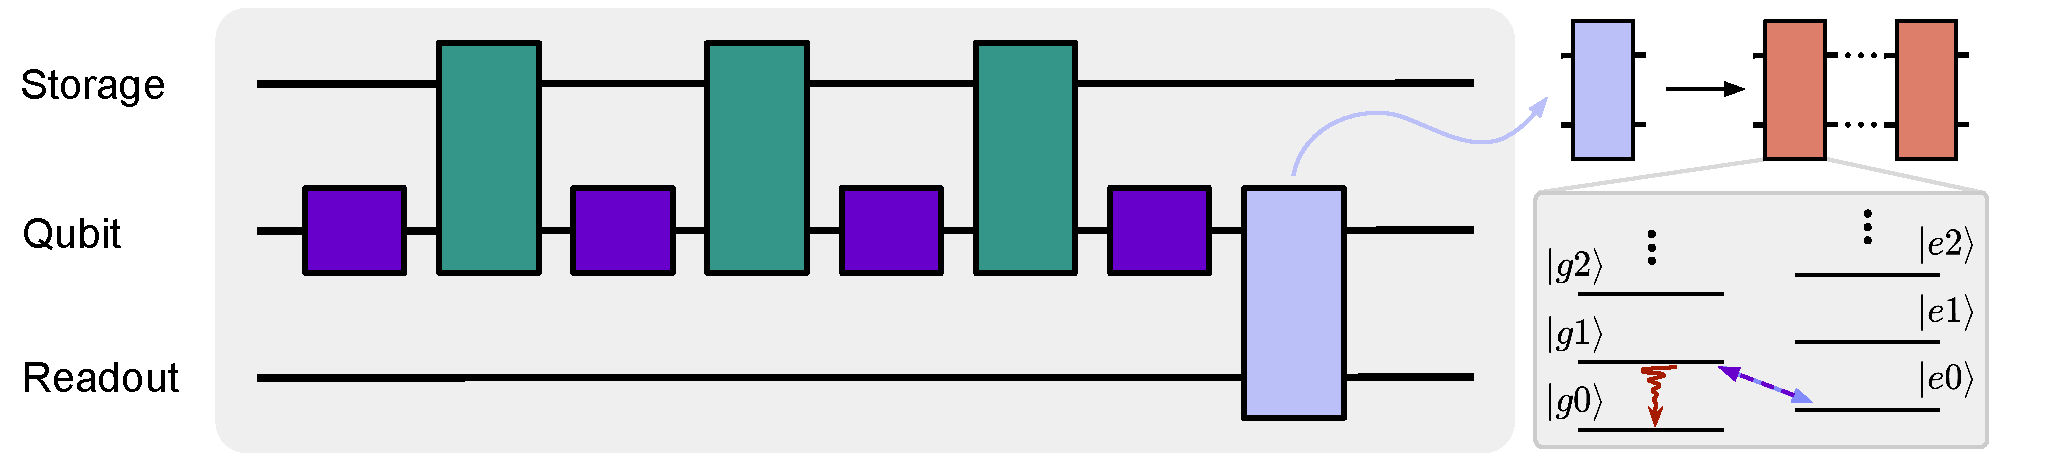
\includegraphics[width=\linewidth]{Figures/5/SBS_Sideband_Reset.pdf}
    \caption{SBS sequence consisting of 3 conditional displacements (teal), 4 qubit pulses (purple),  and unconditional qubit reset (lilac). The reset can be further decomposed into a number of dissipative swap operations based on fluxonium $\ket{e0}\leftrightarrow\ket{g1}$ sideband cooling.}
    \label{fig:5_SBS_Sideband_Reset}
\end{figure}

\clearpage
\subsection{Performance Estimates}

The first check we carried out when assessing the feasibility of a 2D dispersive design was to determine how quickly we can implement a round of SBS (i.e. one quadrature of QEC). We based this on preliminary simulations from our theory collaborators Jonathan Pelletier and Baptiste Royer that indicated\footnote{These simulations aren't yet published, but they show that the maximum storage photon number at which ECD starts to break in simulation is similar or even slightly higher for a fluxonium than for a transmon.} that a fluxonium qubit is not significantly different than a transmon from the perspective of carrying out ECD. As a result (cf. above), we designed our storage-fluxonium system to have a similar dispersive shift and Kerr nonlinearity as the storage-transmon system from Ref. \cite{sivak2023gkp-expt}, and assumed in what follows that we can use a similar photon number (approximately 100-140 storage photons) in ECD. 

\noindent The sequence for SBS is shown in Fig. \ref{fig:5_SBS_Sideband_Reset}: it consists of 4 conditional displacements (CDs), 3 qubit $\pi/2$ rotations, and qubit reset. We assume our CDs take the same time as Ref. \cite{sivak2023gkp-expt} and that our qubit pulses each take 32 ns; meanwhile for reset, we follow Ref. \cite{nordquantique2023gkp-expt} where the authors used $N_{\rm reset} = 2$ dissipative swaps. In our case, our readout has a linewidth of $\kappa_r / 2\pi \approx 16$ MHz, giving a $T_1 \simeq 9$ ns. From here, we estimate our worst case reset time to be $T_{\rm diss. swap} \simeq 132$ ns\footnote{This estimate is based on comparing to the parameters of Ref. \cite{nordquantique2023gkp-expt}; we hope it will be a worst-case value}. In total, the time $\delta t$ that we estimate it will take for an SBS round is:
\begin{align*}
\delta t = T_{\rm sBs}  &= 4T_{\rm pi} + (T_{\rm CD\,1} + T_{\rm CD\,2} + T_{\rm CD\,3}) + \big[N_{\text{reset}}\times T_{\text{diss. swap}}\big] \\ &= 4\times (32) + (470 + 676 + 230) + \Big[2 \times 132\Big] = 1768\, {\rm ns}
\end{align*}
We performed extensive SBS simulations using this value of $\delta t$, assuming different levels of single-photon loss $\kappa_{1s}$. We followed the method from Sec. \ref{sec:2_SBS} by modelling the sequence as an instantaneous QEC channel followed by a loss channel of length $\delta t$ (recall, this gives a lower bound on logical lifetime). For the QEC, we additionally optimized over the error correction parameters (i.e. code size $\Delta$ and small displacements $\epsilon_1, \epsilon_2$) to find the highest logical lifetime $T_L$ at each value of $T_{1s} = 1/\kappa_{1s}$. The results are shown in Fig. \ref{fig:2D_vs_3D_SBS_Comparison}; we plot the dimensionless quantity $T_L/\delta t$ (the number of rounds we can stabilize for) vs. $T_{1s}/\delta t$, the effective storage lifetime in units of the SBS cycle time. We repeat this process for the three cases: (i) a perfect/lossless control qubit (blue); (ii) a control qubit with $T_1 = 1.2$ ms (orange); and (iii) a control qubit with $T_1 = 300$ $\mu$s (green). For each value of $T_{1s}$ we also plot the lifetime of the oscillator $\{\ket{0}, \ket{1}\}$ Fock qubit (black), which is calculated as done in Ref. \cite{royer2020gkp} by $T_L^{\rm fock} = T_{1s}/2$. We see from these results that, at least in simulation, we are able to achieve break-even over the oscillator Fock encoding in all cases. 

\begin{figure}[t]
    \centering
    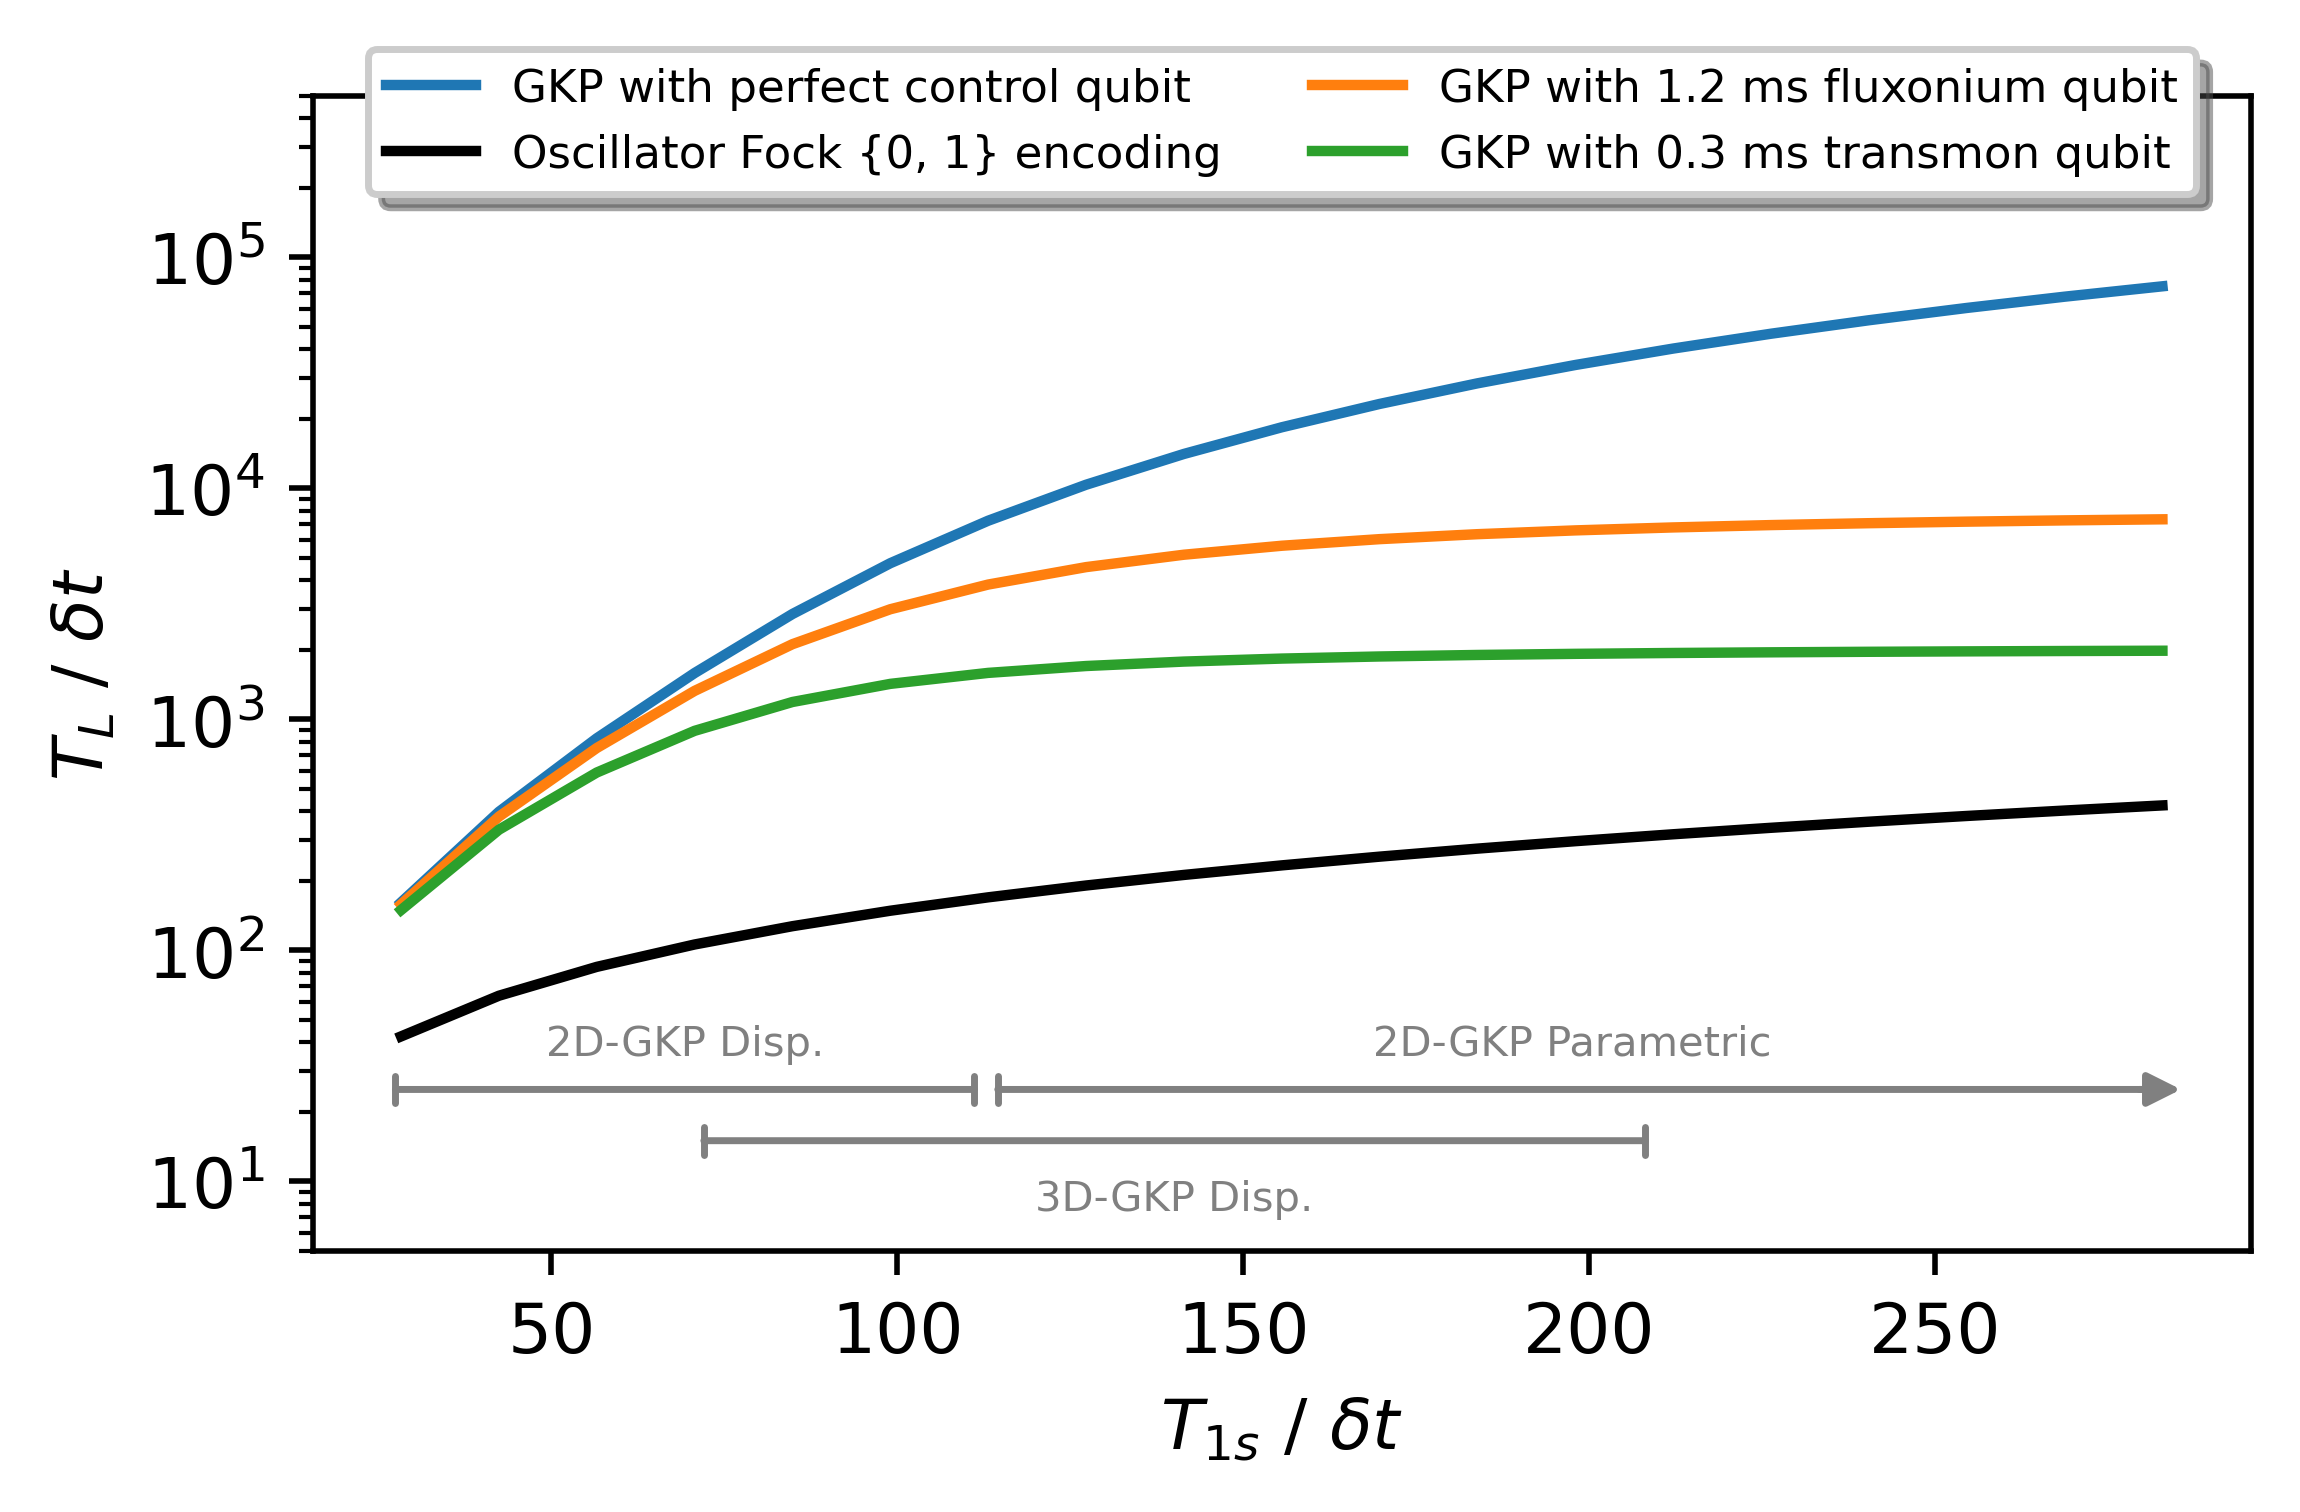
\includegraphics[width=0.8\linewidth]{Figures/5/2D_vs_3D_SBS_Comparison.png}
    \caption{Simulated plot of dimensionless maximum GKP logical lifetime $T_L/\delta t$ from SBS simulations vs. dimensionless storage lifetime $T_{1s}/\delta t$. Here $\delta t$ is the SBS cycle time. We optimized over GKP code parameters to find the maximum $T_L$ at each value of $T_{1s}$, and repeat this for the cases of a lossless qubit, a qubit with $T_1 = 1.2$ ms (e.g. a fluxonium), and a qubit with $T_1 = 300$ $\mu$s (e.g. a transmon). We find that all three cases outperform the bare oscillator Fock encoding here. The ranges in grey are overlaid on the plot assuming $\delta t = 1.7$ $\mu$s and $T_{1s} \in [45, 200]$ $\mu$s for the 2D dispersive experiment; $\delta t = 2.8$ $\mu$s and $T_{1s} \in [200, 700]$ $\mu$s for the 3D dispersive experiment; and finally $\delta t = 400$ ns and $T_{1s} \in [45, 200]$ $\mu$s for the 2D parametric experiment (RAF).}
    \label{fig:2D_vs_3D_SBS_Comparison}
\end{figure}

\noindent Of course, in practice, the logical lifetime will be reduced by many other experimental factors. But, we see from this that it is at least plausible to realize break-even error correction. Finally, since these curves depend only on the product $\kappa_{1s}\delta t$ (i.e. on $T_{1s}/\delta t$), we can use the x-axis to get a sense of the required storage lifetimes for each of our three experiments: the 3D dispersive, the 2D dispersive, and the RAF (2D parametric). We overlay the three expected performance ranges on the plot; what we see is that in the best case scenario, the performance of the 2D dispersive experiment should not be too far behind the ideal performance that we had originally hoped for in our 3D experiment. Additionally, by the same metric, we see that the RAF experiment has the potential to far outperform the other two approaches, and so we expect to be able to achieve state-of-the-art QEC gain here.

Overall, we find that both of our upcoming experiments represent promising pathways towards realizing robust and extensible GKP error correction in 2D. The expect to receive both the RAF and 2D dispersive designs shortly after this writing, and are excited to test these platforms in experiment.  

\printbibliography[heading=subbibliography, title = References]
\printbibliography[heading=subbibliography, title = References]
\clearpage
% % ------------------------------------------------

%%%%% Appendix A: Resonator Fitting %%%%%%
\appendix
\chapter{Appendix: Resonator Fitting\label{ch:AppA}}

As discussed in Ch. \ref{ch:4_3DGKP}, a large part of the experimental work in this thesis involved probing 3D cavity resonators using classical microwave fields --- either to characterize the intrinsic properties (such as resonator internal and coupling losses) or, for the case of our 3D cavity-fluxonium device, to readout the state of the qubit and more broadly interact with the rest of the system. In this appendix, we will briefly derive from first principles the resonance lineshape of a single-mode resonator coupled to a readout transmission line in a so-called reflection configuration. This simple example can be treated theoretically using the input-output formalism, yet is general enough to cover all of the experiments performed in this thesis. 

We start by considering a linear resonator mode $\hat{a}$ with angular frequency $\omega_0$ coupled to a transmission line. The Hamiltonian describing this mode is that of a quantum harmonic oscillator, $\hat{H} = \h\omega_0 \hat{a}^\dagger \hat{a}$. Without the transmission line, the dynamics of $\hat{a}$ are given in the Heisenberg picture by $\partial_t\hat{a} = -i[\hat{a}, \hat{H}] = -i\omega_0\hat{a}$, leading to the familiar oscillatory motion of $\hat{a}(t)$ in the oscillator's phase space. However, if we include losses and coupling to the transmission line, the dynamics are modified in the form of a Heisenberg-Langevin equation \cite{walls1994quantum, gardiner2004quantum, clerk2010introduction}:
\begin{equation}
    \odv*{\hat{a}}{t}(t) = -i\omega_0\hat{a} - \Big(\frac{\kappa_c + \kappa_i}{2}\Big)\hat{a} + \sqrt{\kappa_c}\hat{a}_{\rm in}(t)
    \label{eq:A_heisenberg}
\end{equation}
Here, we include a damping term proportional to the total loss rate $\kappa = \kappa_c + \kappa_i$, where $\kappa_i$ is the \textit{intrinsic loss} of the mode due to uncontrolled interaction with environmental degrees of freedom and $\kappa_c$ is the \textit{coupling loss} to the transmission line (which we as experimenters may control for in design)\footnote{For a full derivation of this Heisenberg-Langevin equation in the context of superconducting circuits, two great expository references are the PhD theses of Audrey Bienfait \cite{bienfait2016thesis} and Steven Touzard \cite{touzard2019thesis}.}. As an example of a setup that implements Eq. \eqref{eq:A_heisenberg}, we may refer back to Fig. \ref{fig:4-3DGKP-schematic-2}(d) of the main text, which shows a schematic of our 3D experiment and, in particular, a model of the cavity resonators. There, the coupling $\kappa_c$ is implemented via a physical pin sticking into the cavity whose length (or rather, distance from the cavity post) determines the coupling strength \cite{axline2016architecture}. The pin is connected to a microwave drive line, which gives rise to the source term $\sqrt{\kappa_c}\hat{a}_{\rm in}(t)$ in Eq. \eqref{eq:A_heisenberg} in terms of the input propagating field $\hat{a}_{\rm in}$ (travelling to the cavity) in the transmission line. We can also have a transmission line field propagating away from the cavity, which we call $\hat{a}_{\rm out}$. 

In circuit QED experiments, we typically interact with readout resonators using a classical field $\alpha_{\rm in}(t)$ associated with a coherent state $\ket{\alpha_{\rm in}}$ in the input transmission line, resulting in a large intra-resonator field $\alpha(t) = \ev{\hat{a}}(t)$. Taking the expectation values on both sides of Eq. \eqref{eq:A_heisenberg}, we thus get $\partial_t \alpha(t) = -i\omega_0\alpha - (\kappa_c + \kappa_i)\alpha/2 + \sqrt{\kappa_c}\alpha_{\rm in}(t)$. Note that by defining a drive amplitude $\epsilon(t) = i\sqrt{\kappa_c}\alpha_{\rm in}(t)$, we can now self-consistently interpret the source term as coming from a Hamiltonian drive $\epsilon(t)(\hat{a} + \hat{a}^\dagger)$ on the system, which also motivates the discussion presented in Sec. \ref{sec:2_control_nonlinearity_drive}. 

If we take a Fourier transform $\mathcal{F}[\bullet]$ of the above equation, we can calculate\footnote{Recalling the definition $\mathcal{F}[\alpha(t)] \equiv \int \alpha(t) e^{i\omega t}dt$, we can derive $\mathcal{F}[\partial_t\alpha(t)] = -i\omega \alpha(\omega)$ via integration by parts.} the frequency domain response:
\begin{equation}
    \alpha(\omega) = \frac{2\sqrt{\kappa_c}}{\kappa_c + \kappa_i - 2i(\omega-\omega_0)} \alpha_{\rm in}(\omega)
    \label{eq:inputoutput-freq-domain}
\end{equation}
This equation gives us the ability to calibrate the mean circulating photon number $\bar{n} = |\alpha|^2$ in the resonator, in terms of the input power $P_{\rm in} = \myhbar\omega |\alpha_{\rm in}|^2$ seen by the device. Specifically, on resonance ($\omega = \omega_0$), we get:
\begin{equation}
    \bar{n} = \frac{4\kappa_c P_{\rm in}}{\myhbar\omega_0(\kappa_c + \kappa_i)^2}
\end{equation}
In the limit $\kappa_i \ll \kappa_c$ that we take for readout, this reduces to $P_{\rm in} = \kappa_c\myhbar\omega_0 \bar{n}/4$. 

\noindent Now, the classical continuity equation for the propagating fields gives rise to the so-called \textit{input-output relation} \cite{clerk2010introduction}, which expresses the resonator mode $\hat{a}$ in terms of the transmission line fields: 
\begin{equation}
    \hat{a}_{\rm in}(t) + \hat{a}_{\rm out}(t) = \sqrt{\kappa_c} \hat{a}(t)
    \label{eq:inputoutput}
\end{equation}
In combination with Eq. \eqref{eq:inputoutput-freq-domain}, this relation allows us to express the reflected coherent output signal $\alpha_{\rm out}(\omega)$ in terms of the input signal $\alpha_{\rm in}(\omega)$ sent in to the resonator. In particular, their ratio defines
\begin{equation}
   S_{11}(\omega) = \frac{\alpha_{\rm out}(\omega)}{\alpha_{\rm in}(\omega)} = \frac{\kappa_c - \kappa_i + 2i(\omega - \omega_0)}{\kappa_c + \kappa_i - 2i(\omega - \omega_0)},
   \label{eq:A_S11_ideal}
\end{equation}
i.e. a reflection coefficient. It tells us the amplitude/phase response of the received output signal  $\alpha_{\rm out}$ in terms of the incident field $\alpha_{\rm in}$ we apply. Note, the choice to call this coefficient ``$S_{11}$'' can be traced back to the S-matrix formalism \cite{kurokawa1965power, gardiner1985input}, which extends the analysis here to multi-port devices, and defines $S_{ij}(\omega) = \alpha_{{\rm out}, i}(\omega)/\alpha_{{\rm in}, j}(\omega)$. We get the same expression if we analyze this setup from an electrical engineering perspective using transmission line theory. In our case, however, we consider just a single-port device, i.e. a cavity resonator in reflection configuration, and so the single S-parameter for the reflected signal is given by $S_{11}(\omega)$; this is also what we measure experimentally using a Vector Network Analyzer (VNA) in the lab.  

In practice, the abstract picture of a transmission line here needs to be physically realized in our microwave setup. Our specific readout setup is shown in Fig. \ref{fig:4-microwave-wiring-diagram}. It is worth noting that we used a (3-port) device called a microwave circulator to implement the ``reflection'' measurement of the cavity in an otherwise ``transmission''-like setup. For a measurement on the VNA, we simply connect its ports to the input and output lines, and the measured response indeed should follow Eq. \eqref{eq:A_S11_ideal}. Of course, there are certain experimental factors that need to be accounted for. These include (i) losses in the microwave cables; (ii) a phase offset of the initial input signal; and (iii) the \textit{propagation delay} (the time it takes for a signal to reach the cavity and return back due to the physical distance between the VNA and the cavity). Also known as the \textit{electrical delay}, this last factor causes the output signal phase to vary with frequency based on the speed of light in the microwave cables. To account for all of these effects, we typically fit experimental data to a modified response function that is given by:
\begin{equation}
   S_{11}^{\rm exp}(\omega) = Ae^{i\phi} e^{2\pi i\lambda\omega} \times \bigg[\frac{\kappa_c - \kappa_i + 2i(\omega - \omega_0)}{\kappa_c + \kappa_i - 2i(\omega - \omega_0)}\bigg]
\end{equation}
where $A$ is an amplitude, $\phi$ is a phase offset, and $\lambda$ encodes the electrical delay. 





Finally, we sometimes also see other experimental non-idealities in a realistic microwave setup such as impedance mismatches in the lines \cite{probst2015efficient} or imperfections in the circulator \cite{rieger2023fano}. These effects can lead to a so-called \textit{Fano resonance} of the cavity, resulting in an asymmetric lineshape of the magnitude response $|S_{11}(\omega)|$. To account for this, we thus typically further modify the fit function to have a complex-valued coupling constant $\kappa_e = |\kappa_e|e^{i\varphi_0}$ \cite{probst2015efficient}. The total linewidth $\kappa$ of the cavity is then defined  in terms of the real part of this coupling constant, $\kappa = \kappa_i + {\rm Re}(\kappa_e)$, and the $S_{11}$ response is given in terms of the full complex-valued $\kappa_e$ via:
\begin{equation}
    S_{11}^{\rm fano}(\omega) = \frac{2i(\omega-\omega_0) + \kappa -  2{\rm Re}(\kappa_e)(1+i\tan(\varphi_0))}{2i(\omega-\omega_0) + \kappa}
    \label{eq:A_S11_fano}
\end{equation}
We used this Fano-corrected fit function when analyzing some of our cavity responses. In particular, following up from a comment made in Ch. \ref{ch:4_3DGKP}, we used this for determining the quality factors $Q_i = \omega_0/\kappa_i$ of our 3D cavity resonators. An example of such a response for our bare ``Mark II'' cavity storage resonator (i.e. without the fluxonium chips inserted) is plotted below, from which we extract the characteristic lifetime $T_1 = 1/\kappa_i \approx 765$ $\mu$s. 
\begin{figure}[h]
    \centering
    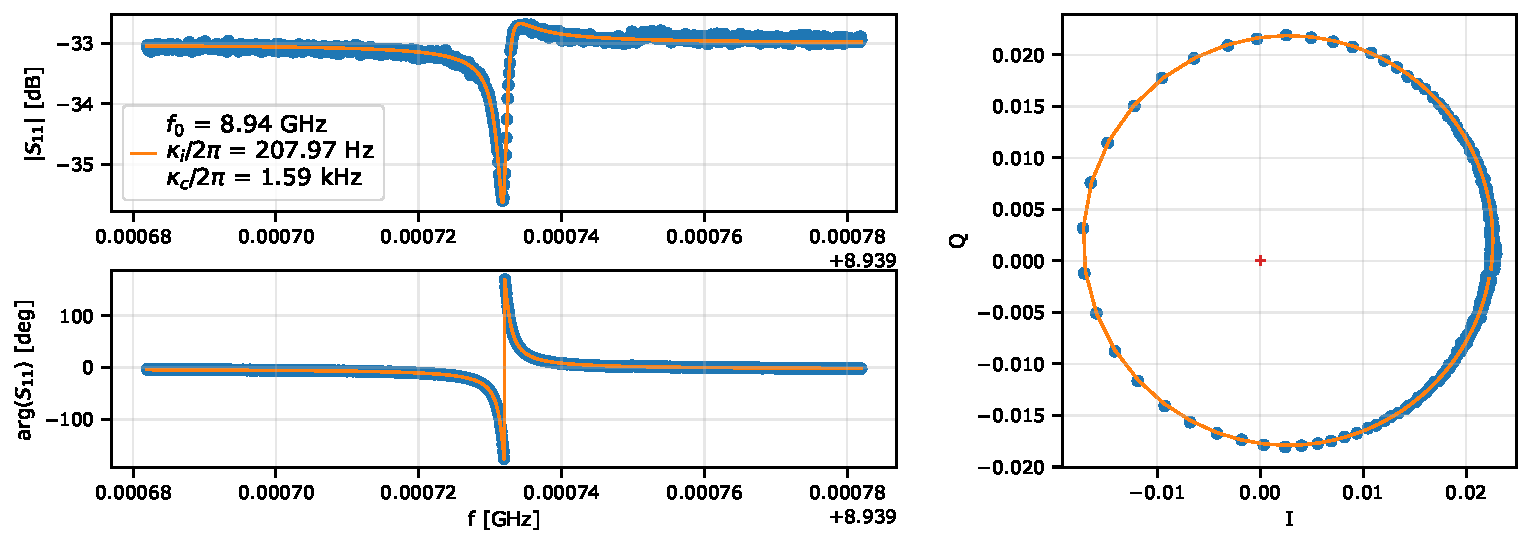
\includegraphics[width=\linewidth]{Figures/A/Storage_Res_S11_Fit.pdf}
    \caption{$S_{11}$ magnitude and phase response of our Mark II storage cavity plotted vs. frequency $f = \omega/2\pi$. From a fit to Eq. \eqref{eq:A_S11_fano}, we extract the resonator frequency $f_0 = \omega_0/2\pi$ and the internal and coupling losses $\kappa_i$ and $\kappa_c \equiv {\rm Re}(\kappa_e)$. The internal loss determines the intrinsic quality of the resonator, from which we can extract a lifetime $T_1 = 1/\kappa_i \approx 765$ $\mu$s.}
    \label{fig:A_Storage_Res_S11_Fit}
\end{figure}
\printbibliography[heading=subbibliography, title = References]
\clearpage
% ------------------------------------------------

%%%%% Appendix B: Making 3D Cavities %%%%%%
\chapter{Appendix: Fabricating High-Q 3D Cavities \label{ch:AppB}}

In this brief appendix, we will review the standard operating procedures that we followed when fabricating aluminium 3D cavity resonators. Our overall procedure was developed through several iterations of cavities and so the version we present here is the final process that we eventually converged on. All of the 3D cavities used in this thesis were machined out of high-purity bulk aluminium with a grade of 5N5 (99.9995\% purity), as is typical for Al post cavity designs in past circuit QED experiments \cite{reagor2013reaching}. After designing and simulating the cavity, we submitted our specifications to the MIT Central Machine Shop for the actual machining of the device. Once we received the final machined cavities, the next steps were cleaning and etching; we performed both of these in the MIT.nano cleanroom.

For cleaning, we first dipped the cavity into a beaker of 1-methyl-2-pyrrolidone (NMP) for approximately a minute, until the color of the NMP changed to brown (removing any dirt or oils on the cavity left over from machining). We then did a more thorough cleaning by sequential sonication of the sample in (fresh) NMP, then acetone, and finally isopropyl alcohol (IPA). The solvents are chosen in the typical order of decreasing `strength' in order to remove machine oils and residues. We sonicate at a medium setting for 5 minutes each, transferring quickly between beakers to prevent solvent residues forming in air. After the IPA, we finally blow dry the sample with $N_2$ gas. 

Once the cavity is clean, we next proceed with the critical step of chemical etching in acid. The purpose of the etch is to treat surface imperfections and roughness of the aluminium, and it is a crucial ingredient for achieving high quality factor 3D resonators. We etch using the commonly-available Transene Aluminium Etchant Type A, which is a mix of nitric and phosphoric acid. The acid is heated to 50$^\circ$C using a hot plate and is temperature-controlled via a PID loop and thermometer. In our case, we placed the cavity in a teflon basket before lowering it into the acid bath along with a magnetic stir bar. We etched for 4 hours in total but replaced the acid every 45 minutes to prevent saturation. In each segment, we see the color of the acid change as the reaction proceeds as well as bubbles forming. We found it to be important to reorient the cavity within the acid in each segment to allow the bubbles to rise to the surface (and not get trapped within the cavity or below it); in our experience, this led to the best and most uniform etches, which indeed we saw translated into higher resonator lifetimes. 

Following the acid treatment, we rinse the cavity in DI water for 5 minutes or more and then blow dry with $N_2$ gas. At this point, the cavity should have high lustre and the grain boundaries of the aluminium should be clearly visible. We finally perform another round of sonication in acetone and IPA for 3 minutes each before finally blow drying in $N_2$ again\footnote{We note that this process is slightly different to that in Ref. \cite{reagor2013reaching}, where the authors rinsed cavities in methanol following the acid etch. We did not try this yet, but leave it as an avenue for future 3D cavities we make.}.


\printbibliography[heading=subbibliography, title = References]
\clearpage
% ------------------------------------------------


%%%%% The End %%%%%%
%\cleardoublepage
%\phantomsection
%\addcontentsline{toc}{chapter}{References}
\sloppy
\end{document}